%% TODO: finish application to IBM. 2 (and maybe 3 and 4 species). Habitat loss. Single pp-pair from large simulation, and functional grouping.
%%  			> 3 species Jhat not wokring (for chain - ensemble_K estimates are too large. Why? Try other 3sp nets? Other options...)

%% TODO: ODE application to Holling model - quaility versus noise and sampling, and Range sampling (conclude nice concept but very sucetible to noise)

%% TODO:  fill in [REF]S
%% TODO:  sort out noise: check equations(outline.pdf and email to MG dated 12/12/14) & simulations.
%% TODO:  edit FR example figure
%% TODO:  examples section - with inference

%% TODO: be able to derive Timme method on paper - look at matrix calculus notation
%% TODO: conduct local stability analysis for models, and reduce parameter space by subsitution.
%% TODO: include stability analysis in section on simulation procedure?

%% TODO: refer to cite{kefi2012more} if extending this to non-trophic interactions...

%% TODO: search and replace Holling and linear with type I and II

\section{Introduction}
%\section{Motivation}
\label{sec:motivate_interactions}
% more emphasis on interspecific interactions.

In this chapter we develop a methodology for the estimation of species interaction strengths from population dynamics data. The primary motivation for this task was provided in section \ref{sec:intro_inference}. Throughout this thesis we have seen that species interactions play a key role in driving the structure and dynamics of simulated communities. In particular strong interactions have been shown to increase the temporal variability of population dynamics. They have also represented one main difference between communities under the two types of habitat loss (HL) studied: random and contiguous. Random HL has been shown to present barriers to the motion of individuals, which reduced species interaction strengths. In contrast contiguous HL was found to increase interaction strengths by compressing individuals into a smaller region of space. These changes in interaction strengths partly explained the different responses of communities to the two types of HL. For example contiguous HL produce more extinctions, and did not result in trophic collapse of communities to the same extent as random HL. The important role of interaction strengths in understanding the results of previous chapters, further motivates the study of methods to quantify them. Previously the metric IS (equation \eqref{eq:is3}) has been used. However this metric requires accurate knowledge of all interaction frequencies and species abundances. The method developed in this chapter requires only the latter, although abundance time series are required rather than snapshots. The method also makes explicit the connection between community dynamics and interaction strengths, by fitting a population dynamics model.   

%Plankton mention here? (Or only in intro?) Mention Timme here - yes! Mention interaction types other than antagonism?

The original intention for this chapter was to obtain an empirical dataset with high resolution abundance time series \emph{and} quantified interaction strengths. Such a dataset would provide the ideal test of the methodology presented. However such data was not forthcoming, either in the form of experimental mesocosm data, or that sampled from a real-world community. Therefore the methodology is developed with application to simulated community dynamics. Such an approach ensures knowledge of the interactions involved in the study system, and allows detailed analysis of the results over a range of experimental conditions. Section \ref{sec:methods_si} provides full details of the methodology, which is summarised in figure \ref{fig:method_flow}.  In section \ref{sec:results} interaction strengths are inferred from two species predator-prey dynamics, simulated using ordinary differential equation models. The accuracy of the inferred results are evaluated for two different simulation models, under noise and using different sampling regimes. In section \ref{sec:ibm} interaction strengths are inferred from community dynamics simulated using the IBM model. Two, three, five, and sixty species communities are investigated. In section \ref{sec:si_discussion} the performance and limitations of the methodology are discussed. Finally in section \ref{sec:si_conc} further developments are considered, including the potential for applications to empirical data. Although the focus of this chapter is on antagonistic predator-prey interactions, the intention is that this methodology could be extended to infer other interaction types (mutualism and competition). 

    %We described how population dynamics are simulated (section \ref{sec:models}); how species interactions are inferred from these dynamics (sections \ref{sec:def_GLV} and \ref{sec:timme}); and define the quantities that these estimates are compared to (section \ref{sec:interaction_strength}).

\section{Methodology}
\label{sec:methods_si}

%% reorder and state where IM is given for simulation..

\begin{figure}[h]
\centering 
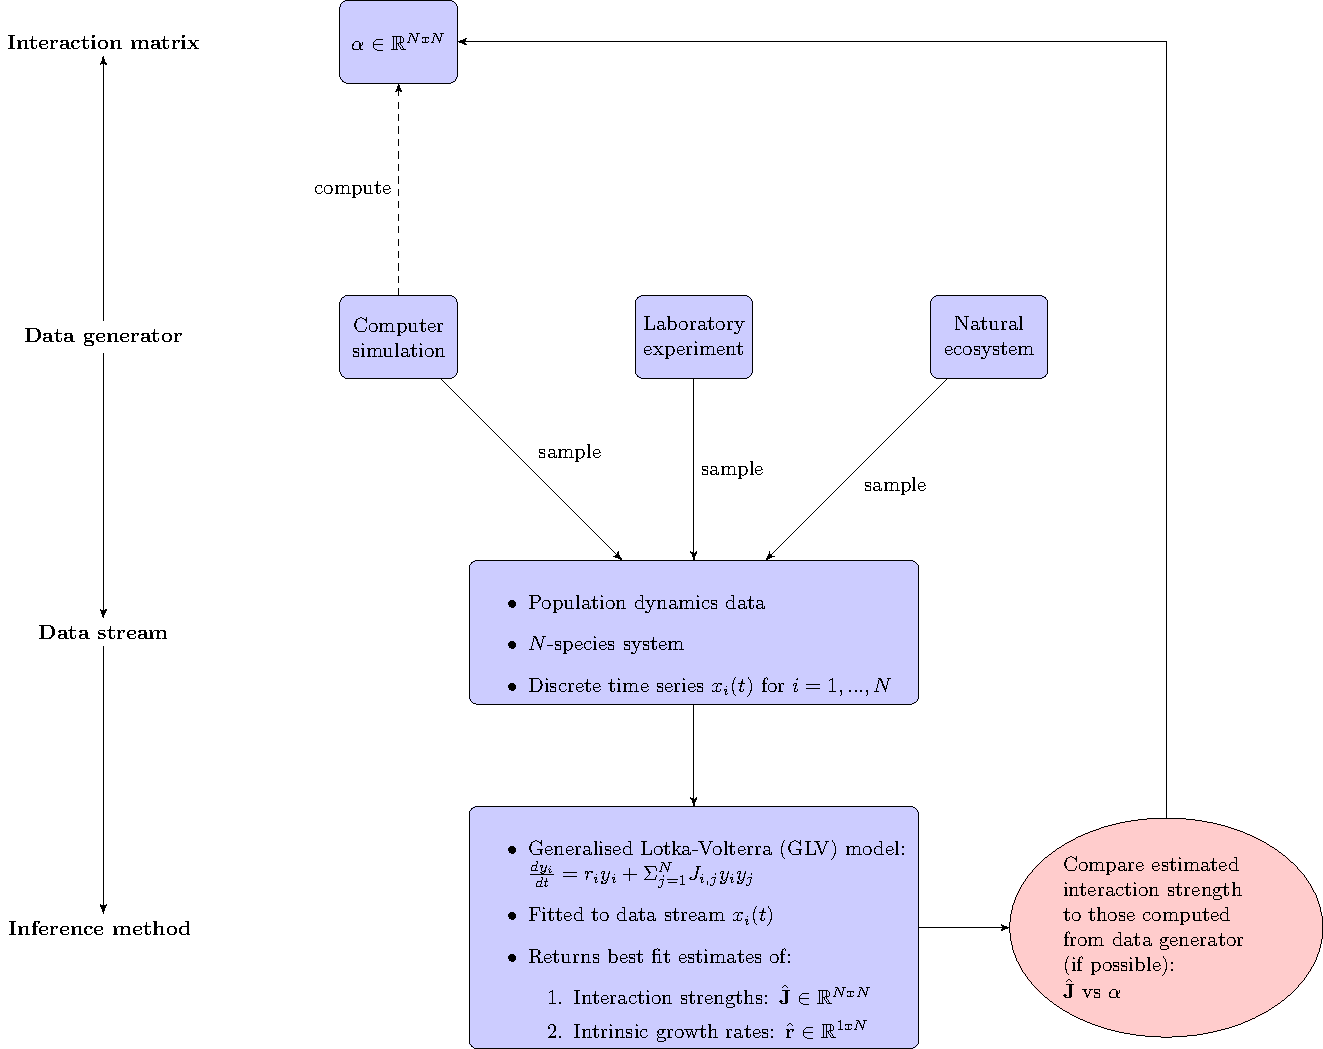
\includegraphics[width=\textwidth]{{{flow_chart/flow_chart}}}
\caption[Schematic of inference methodology.]{Methodological approach to estimate species interaction strengths from population dynamics, and evaluate the resulting estimates.} 
\label{fig:method_flow}
\end{figure}

The methodological approach to the estimation of species interaction strengths is depicted in figure \ref{fig:method_flow}. The starting point is a \emph{data generator} from which samples of population sizes are taken over a given period of time. The \emph{data generator} may be a natural ecosystem, or laboratory experiment, from which we wish to determine which species are interacting and quantify the strengths of those interactions. Given that the interaction strengths between species are not know \emph{a priori} for a natural system (hence the motivation for the current investigation), in this chapter we use computer simulations of interacting species as a \emph{data generator} to develop the methodology. Sampling from the \emph{data generator} produces a \emph{data stream}, which is an N-dimensional time series $x_i(t)$ representing the population size of each of the $N$ species sampled at discrete time points $t$. Examples of \emph{data generators} and \emph{data streams} are plotted in section \ref{sec:method_examples}. An \emph{inference method} is then applied to the sampled time series, producing estimates of the strength of interactions between all pairings of the $N$ species in the original \emph{data generator}. The \emph{inference method} used here involves fitting a \emph{generalised Lotka-Volterra} (GLV) model, which is defined in section \ref{sec:def_GLV}. The procedure used to fit the GLV to time series is adapted from work by Shandylia and Timme \cite{shandilya2011inferring}, and is detailed in section \ref{sec:timme}.

The performance of the \emph{inference method} is evaluated by comparing its results to known properties of the \emph{data generator}. In the first part of this chapter (section \ref{sec:results}) ordinary differential equation (ODE) models are used as \emph{data generators} to simulate population dynamics. These ODE models are defined in section \ref{sec:models} and are useful here because they allow analytic calculation of \emph{a priori} interaction strengths. Therefore we are able to compare the interaction strengths estimated by the \emph{inference method} (the GLV fit), to those calculated directly from the \emph{data generator} (the ODE model). To calculate interaction strengths from the ODE models we use a metric called the \emph{interaction matrix} ($\alpha$) \cite{berlow2004interaction}. The definition of $\alpha$ and its interpretation are given in section \ref{sec:interaction_strength}.

Later in the chapter (section \ref{sec:ibm}) the IBM model, familiar from previous chapters, is used as the \emph{data generator}. Unlike the ODE models the IBM does not allow \emph{a priori} calculation of interaction strengths. However we do know \emph{which species interact} in the IBM, because this is specified by the underlying interaction network. Therefore one test of the \emph{inference method} when applied to the IBM is to see if it correctly identifies which species are interacting. Also, in the IBM, interaction strengths between species emerge as a result of interactions between individuals in the landscape. We have seen previously that the strength of these species interactions can be quantified from simulation output by the metric IS (defined in section \ref{sec:def_iss}). Therefore the performance of the \emph{inference method} can also be evaluated by comparing IS and $\alpha$. More details on the use of the IBM as the \emph{data generator} are given at the beginning of section \ref{sec:ibm}. In the rest of this section full details of the methodology as applied to ODE \emph{data generators} are provided, in the order introduced above (and corresponding to the flow chart in figure \ref{fig:method_flow}).

%To summarise our methodology, we simulate population dynamics then sample these dynamics and fit a . The fitted GLV parameters give us estimates of the species interaction strengths (and other parameters), which we then compare to those used in the original simulation. The details of all the stages are given below. In section \ref{sec:interaction_strength} the \emph{interaction matrix} (IM) is introduced. The IM is the metric used to quantify the strength of species interactions and is key to this chapter. We also introduce the \emph{generalised Lotka-Volterra} (GLV) model, and show that this model has constant interaction strengths, given by the coupling matrix $J$. In section \ref{sec:models} we give a general framework for ODE predator-prey modelling, and derive the two models that we use to simulate population dynamics. We then discuss, in section \ref{sec:simulation_method} the details of how these models are simulated \emph{in silico}, including the selection of model parameters. Section \ref{sec:timme} gives the details of the numerical method we use for fitting the GLV model to sampled population dynamics. In section \ref{sec:method_examples} we give an example of the full methodology in action.

\subsection{Data generator: ordinary differential equation models}
\label{sec:models}
%LINEAR IS SAME AS GLV!!
%% Parameter choices. Euler method. Timestep. Extinction boundary contiditions.
%% Conventional to use N,P for predator prey, however our terminology allows easy extension to larger systems..(refer forwards to this)
%% re-order this - good choice first!

In section \ref{sec:results} ordinary differential equation (ODE) models are used as the \emph{data generator}. The results presented in this chapter are all for \emph{antagonistic} communities. Therefore each inter-specific interaction is modelled as predator-prey type. The ODE modelling framework defined below is specific to predator-prey systems, but may be extended  to model other interaction types (e.g. competition and mutualism). For an $N$ species predator-prey system the ODE model is defined by $N$ coupled first-order differential equations, which take the general form
\begin{equation}
\frac{dx_i}{dt} = G_i(x_i) + \Sigma_{j=1}^N C_{ij}(x_i,x_j),
\label{eq:general_form}
\end{equation}
%
where $x_i$ represents the population density (or biomass/abundance) of species $i$; $G_i(x_i)$ is the intrinsic growth function of species $i$; and $C_{ij}(x_i,x_j)$ is a function that defines the coupling (or interaction term) between species $i$ and $j$. The form of \eqref{eq:general_form} is sufficiently general that most common models from the population dynamics literature may be expressed in this way by making suitable choices for $C$ and $G$. Examples of such models include those of Holling \cite{holling1959some}, Rosenzweig and MacArthur \cite{rosenzweig1963graphical}, Arditi \cite{arditi2012species}, and Lotka-Volterra \cite{volterra1926,lotka1925elements}. In section \ref{sec:results} the results presented are for two species systems, for which the full model may be expressed as

\begin{eqnarray}
\frac{dx_0}{dt} &=& G_{0}(x_0) + a_{01}x_1H(x_0,x_1),  \nonumber \\[10pt]
\frac{dx_1}{dt} &=& G_{1}(x_1) + a_{10}x_1H(x_0,x_1)
\label{eq:two_species}
\end{eqnarray}
%
where species $x_0$ and $x_1$ are the population densities of the prey and the predator species respectively; and we have expressed the coupling term in terms of $H(x_0,x_1)$, the \emph{functional response} (FR) of the predator, which is multiplied by constant coupling coefficients $a_{ij}$. The FR defines the per-capita rate of consumption of the predator, and is a key feature of such predator-prey models \cite{barraquand2014functional,jost2000identifying}. The coefficients $a_{01}$ and $a_{10}$ are negative and positive respectively, such that the prey losses biomass, and the predator gains biomass as a result of the interaction. These coefficients may be used to introduce asymmetry into the interaction terms. For example it is common to choose $|a_{01}| > |a_{10}|$, to model the inefficiency of the predator in the conversion of biomass from the prey. For the intrinsic growth functions we use the functional forms  

%the $G_i(x_i)$ are the intrinsic growth functions of each species; the $a_{ij}$ are constant coefficients and $H(x_0,x_1)$ is the functional response (FR) of the predator. This form is standard in the literature [REFS] and many models may be expressed in this way by choosing different functional forms for $G$ and $H$. 

\begin{eqnarray}
G_0(x_0) &=& r_0x_0\left(1-\frac{x_0}{K_c}\right)  \\[10pt]
G_1(x_1) &=& r_1x_1,
\label{eq:intrinsic_growth}
\end{eqnarray}
%
where $r_0 > 0$ and $r_1 < 0$ are the intrinsic growth rates of the prey and predator respectively; and $K_c$ is the carrying capacity of the prey species. Therefore the predator has an exponential intrinsic mortality, whereas the prey species has logistic intrinsic growth. These use of these functional forms to model intrinsic growth was made popular by Rosenzweig and MacArthur \cite{rosenzweig1963graphical}. The justification for the use of logistic growth in the prey but not the predator is that it models a finite availability of resource (be it space, light, nutrients etc.) to the prey species, whereas the resource availability to the predator (i.e. $x_0$) is modelled directly. However some models, especially those of marine systems, have included similar limiting terms in the intrinsic growth function of the predator species \cite{mitra2009closure}. These limitations are known as \emph{closure terms}, and they attempt to model feeding effects on the predator from species in higher trophic levels which are not modelled directly. For simplicity we choose not to include closure terms in our modelling framework. 

The functional response (FR) defines the per-predator rate of consumption of prey. We focus on the forms proposed by Holling in the 1950s \cite{holling1959some}, which remain widely used in this field \cite{hastings2013population}. However it is worth noting that various other forms have been proposed and there is an ongoing debate about which form is most appropriate in different situations \cite{barraquand2014functional,jost2000identifying} (see discussion in section \ref{sec:intro_inference}). There are three types of Holling FR, referred to as types I, II, and III. These can be expressed as

\begin{eqnarray}
H_I(x_0,x_1) &=& x_0,  \label{eq:h1} \\[10pt]
H_{II}(x_0,x_1) &=& \frac{x_0}{x_0 + K_s},  \label{eq:ho2} \\[10pt]
H_{III}(x_0,x_1) &=& \frac{x_0^2}{x_0^2 + K_s^2},
\end{eqnarray}
%
where $x_0$ is the prey density, and $K_s$ is the saturation constant for the predator, giving the prey density at which the per-predator consumption rate reaches half-maximum. We choose to narrow our investigation by focusing here on the first two forms: Holling type I and type II. Based on the choice of FR we obtain two distinct simulation models, which we refer to as the \emph{type I} and \emph{type II} models.

\paragraph*{The type I model} uses the FR given by \eqref{eq:h1}. This is the simplest of the Holling functions. The per-predator predation rate is linear in prey-density. The full \emph{type I} model is given by

\begin{eqnarray}
\frac{dx_{0}}{dt} &=& r_0x_0\left(1-\frac{x_0}{K_c}\right) + a_{01}x_0x_1 \label{eq:1lin_mod1} \\[10pt]
\frac{dx_{1}}{dt} &=& r_1x_1 + a_{10}x_0x_1 \label{eq:1lin_mod2}, 
\end{eqnarray}
%
The type I model may be rescaled in order to reduce the number of parameters. This makes the local stability analysis simpler, and reduces the dimension of the search space when probing the equations numerically via simulation. We introduce the following non-negative parameters
%\begin{eqnarray}
%\tilde{t} &=& -r_1 t, \\[10pt]
%A &=& \frac{r_0}{r_1}, \\[10pt]
%B &=& \frac{a_{01}}{r_1}, \\[10pt]
%C &=& \frac{-a_{10}K_c}{r_1}, \\[10pt]
%\tilde{x}_0 &=& \frac{x_0}{K_c}, \\[10pt]
%\tilde{x}_1 &=& x_1,
%\end{eqnarray}
\begin{eqnarray}
\tilde{t} &=& -r_1 t, \qquad A = \frac{r_0}{r_1}, \qquad B = \frac{a_{01}}{r_1}, \\[10pt]
C &=& \frac{-a_{10}K_c}{r_1}, \qquad \tilde{x}_0 = \frac{x_0}{K_c}, \qquad \tilde{x}_1 = x_1,
\end{eqnarray}
%
such that equations \eqref{eq:1lin_mod1} and \eqref{eq:1lin_mod2} may be written

\begin{eqnarray}
\frac{d\tilde{x}_{0}}{d\tilde{t}} &=& A\tilde{x}_0(1-\tilde{x}_0) - B\tilde{x}_0\tilde{x}_1 \label{eq:lin_mod1} \\[10pt]
\frac{d\tilde{x}_{1}}{d\tilde{t}} &=& -\tilde{x}_1 + C\tilde{x}_0\tilde{x}_1 \label{eq:lin_mod2}, 
\end{eqnarray}
%
which is the same \emph{type I} model, but expressed in a reduced parameter space. Henceforth for simplicity we drop the \emph{tildes} unless otherwise stated. The equilibrium population densities are given by

\begin{equation}\label{eq:lin_mod_eq}
x_{0}^{*} = \frac{1}{C}, 
\qquad
x_{1}^{*} = \frac{A}{B}\left(1 - \frac{1}{C}\right) , 
\end{equation}
%
such that $x_0^*$ is always positive since $C \in \mathbb{R}^+$; and $x_1^*$ is positive when $C>1$. This is a requirement for physical realism, since it is not possible to have negative populations of species. In most applications it is also required that the equilibrium is stable, to allow for the coexistence of species (i.e. \emph{persistence}, see section \ref{sec:closed_communities}). The equilibrium is locally stable if the eigenvalues of the \emph{Jacobian} matrix ($\mathbb{J}$) have negative real parts. The Jacobian for this model, evaluated at the equilibrium, is given by
\begin{equation}\label{eq:jac1}
\mathbb{J}_{type\ I} = 
\begin{bmatrix}
-A/C & -B/C \\ A/B(C-1) & 0
\end{bmatrix}  	.
\end{equation}
%
We use conditions on the model Jacobian to guide realistic parameter selection when simulating the model. Parameter selection is discussed further section \ref{sec:param_selection}. 


\paragraph*{The type II model} uses the FR given by \eqref{eq:ho2}. The per-predator predation rate is a non-linear function of prey density. The type II FR models predator saturation - individuals take a certain amount of time to process and digest prey - such that the predation rate does not increase linearly as the availability of prey increases. Instead the response curve flattens out, or saturates, at high prey densities (see figure \ref{fig:fr_example} below). The full \emph{type II} model is given by

\begin{eqnarray}
\frac{dx_{0}}{dt} &=& r_0x_0\left(1-\frac{x_0}{K_c}\right) + \frac{a_{01}x_0x_1}{x_0 + K_s} \label{eq:2_mod1} \\[10pt]
\frac{dx_{1}}{dt} &=& r_1x_1 + \frac{a_{10}x_0x_1}{x_0 + K_s} \label{eq:2_mod2}, 
\end{eqnarray}
%
We may perform a similar rescaling as we did with the \emph{type I} model to reduce the number of parameters. We introduce the following non-negative parameters
%\begin{eqnarray}
%\tilde{t} &=& -r_1 t, \\[10pt]
%A &=& \frac{r_0}{r_1}, \\[10pt]
%B &=& \frac{a_{01}}{r_1K_c}, \\[10pt]
%C &=& \frac{-a_{10}}{r_1}, \\[10pt]
%D &=& \frac{K_s}{K_c}, \\[10pt]
%\tilde{x}_0 &=& \frac{x_0}{K_c}, \\[10pt]
%\tilde{x}_1 &=& x_1,
%\end{eqnarray}
\begin{eqnarray}
\tilde{t} = -r_1 t, \qquad A = \frac{r_0}{r_1},  \qquad B = \frac{a_{01}}{r_1K_c}, \qquad C = \frac{-a_{10}}{r_1}, \\[10pt]
D = \frac{K_s}{K_c}, \qquad  \tilde{x}_0 = \frac{x_0}{K_c}, \qquad \tilde{x}_1 = x_1,
\end{eqnarray}
%
such that equations \eqref{eq:2_mod1} and \eqref{eq:2_mod2} may be written

\begin{eqnarray}
\frac{d\tilde{x}_{0}}{d\tilde{t}} &=& A\tilde{x}_0(1-\tilde{x}_0) - \frac{B\tilde{x}_0\tilde{x}_1}{\tilde{x}_0 + D} \label{eq:hol_mod1} \\[10pt]
\frac{d\tilde{x}_{1}}{d\tilde{t}} &=& -\tilde{x}_1 + \frac{C\tilde{x}_0\tilde{x}_1}{\tilde{x}_0 + D} \label{eq:hol_mod2}, 
\end{eqnarray}
%
which defines the \emph{type II} model with seven instead of seven parameters. Again we drop the \emph{tildes} unless otherwise stated. The equilibrium populations for this model are given by

\begin{equation}\label{eq:hol_mod_eq}
x_{0}^{*} = \frac{D}{C-1},
\qquad 
x_{1}^{*} = \frac{ACD(C-1-D)}{B(C-1)^2} , 
\end{equation}
%
such that $x_0^* > 0 $ if $C > 1$, and $x_1^* > 0 $ if $C - D > 1$. These conditions provide constraints on the possible choice of parameters. Further constraints are imposed by the aforementioned conditions on the trace and determinant of the \emph{Jacobian}. For this model the Jacobian, evaluated at the equilibrium, is given by

\begin{equation}\label{eq:jac2}
\mathbb{J}_{type\ II} = 
\begin{bmatrix}
A\left(\frac{-CD +C -D + 1}{C(C-1)}\right) & \frac{-B}{D} \\[10pt] \frac{A(C-1-D)}{B} & 0
\end{bmatrix}  	.
\end{equation}
%
Parameter selection for this model is also discussed in section \ref{sec:param_selection}. 


\subsection{Inference method: generalised Lotka-Volterra model}
\label{sec:def_GLV}

Having simulated population dynamics, using the ODE \emph{data generators} just defined, we then sample from the simulation output to produce a discrete time series $x_i(t)$ for each species $i$. The time series represents the population size of that species at discrete points in time. Together the $x_i(t)$ for all species represent the \emph{data stream}. To estimate species interaction strengths we fit a \emph{generalised Lotka-Volterra} (GLV) model to the data stream. The GLV model is the extension of the Lotka-Volterra equations to $N$ species, and is given by

\begin{equation}
\frac{dy_i}{dt} = r_iy_i + \Sigma_{j=1}^N J_{ij}y_iy_j,
\label{eq:glv}
\end{equation}
%
where $y_i$ is the population density of species $i$; $r_i$ is the intrinsic growth rate; $N$ is the number of species; and $J_{ij}$ is the coupling between species $i$ and $j$. Specifically $\mathbf{J}$ is the GLV coupling matrix, not to be confused with the \emph{Jacobian} $\mathbb{J}$ used in local stability analysis. All parameters here ($r_i$ and $J_{ij}$) may take positive or negative values. The estimated values of $J_{ij}$, obtained from the model fit, give estimates of species interaction strengths. The $J_{ij}$ values also define the type of interaction between two species. For example if $J_{ij} < 0$ and $J_{ji} > 0$, this suggests that species $j$ predates on species $i$. The diagonal elements of the coupling matrix ($i=j$) give estimates of intra-specific interactions.

Our choice of the GLV model reflects its simplicity and therefore its breadth of application. As seen from equation \eqref{eq:glv} there are no assumptions about species roles built into the functional forms of the model. That is, before the model is parametrised, it does not specify if species $i$ is a prey or a predator. Therefore when the model is fitted to a \emph{data stream} the roles of predator and prey emerge from the fitted model parameters. This feature of the model is especially desirable for the application of our methodology to larger multi-trophic systems (section \ref{sec:ibm}). 

The \emph{type I} model from section \ref{sec:models} can be expressed as a GLV model by assigning the parameters as follows
\begin{eqnarray}
r_0 = A, \qquad r_1 = -1, \qquad J_{00} = A, \\[10pt]
J_{01} = -B, \qquad J_{10} = C, \qquad J_{11} = 0.
\end{eqnarray}
%
Therefore the GLV model should be able to exactly fit to a \emph{data stream} derived from the \emph{type I} model. In this instance we would be able to recover the interaction strengths (and other model parameters) with high accuracy. In practice such `perfect' results are hampered by the presence of noise and sparsity of sampling from the data generator (see results in section \ref{sec:res_glv}). In contrasts the \emph{type II} model cannot be expressed in GLV form because of the non-linear functional response (equation \eqref{eq:ho2}). Therefore fitting the GLV model to a \emph{data stream} derived from the \emph{type II} model can at best produce approximations of the true interaction strengths and rate parameters (see results in section \ref{sec:res_hii}). However such a situation represents an important test of the inference method, since functional responses found in nature likely take some non-linear form \cite{arditi2012species}.  
 
\subsection{Inference method: model fitting}
\label{sec:timme}

%% Dealing with extinctions. Range sampling - diagrams!!
%% make use of GLV more explicit

To fit the GLV model to sampled \emph{data streams} we use the numerical method developed by Shandylia and Timme \cite{shandilya2011inferring}. We include here the derivation of their method, but slightly simplified because in their application each \emph{node} represented a chaotic oscillator with three-dimensional dynamics. In our application each node represents a species, with one-dimensional dynamics. The method gives `best fit' estimates of the GLV parameters, which were introduced in section \ref{sec:def_GLV}. Conceptually these estimates are obtained by minimising the error between time derivatives calculated from the \emph{data stream}, and those predicted by the model given the \emph{data stream}. Suppose we that we are trying to fit a population model that, for each species $i$, takes the general form

\begin{equation}\label{eq:timme1}
 \dot{y}_i = r_if_i(y_i) + \Sigma_{j=1}^{N}J_{ij}g_{ij}(y_i,y_j),\\
\end{equation}
%
where $\dot{y}_i = \frac{dy_{i}}{dt}$; $N$ is the number of species in the system and $i,j$ index the species. The $r_i$ and $J_{ij}$ are constants coefficients, whereas $f_i$ and $g_{ij}$ are known functions. This form looks familiar, indeed all of the ODE models discussed so far in the chapter may be expressed in this form. There is an intrinsic growth term, and a linear sum of pairwise interaction terms. To express the GLV model (equation \ref{eq:glv}) in this form, we let

\begin{eqnarray}
f_i(y_i) &=& y_i \\
g_{ij}(y_i,y_j) &=& y_iy_j.
\end{eqnarray}
%
It would be possible to use this method to fit models other than the GLV, so long as the functions $f_i$ and $g_{ij}$ are \emph{known and parametrised}. Since the functions $f_i$ and $g_{ij}$ are known there are $N+1$ unknowns in equation \eqref{eq:timme1}: $r_i$ and $J_{i,j}$ for $j=1,...,N$. Therefore, if we knew the exact values of $\dot{y_i},y_i$ and the $y_j$'s, at $N+1$ time points, then we could solve the equation for $r_i$ and the $J_{i,j}$'s. However in any practical application our knowledge of the system is not \emph{exact}; the system is subject to noise; and the model may be an imperfect description of the dynamics. So the equation cannot be solved exactly. We must look for an approximate solution. To do this the full \emph{data stream} is sampled at $M+1$ time points $t_m$ for $m \in {1,..,M,M+1}$. Therefore we obtain $M+1$ data samples $x_i(t_m)$ to which the model is fitted. 

The data samples are used to construct estimates for the states($\hat{y}_i$ and their time-derivatives $\hat{\dot{y}}_i$ at $M$ intermediate time points, for every species $i$. The time-derivatives are estimated to first order, taking the finite difference between samples at two consecutive time points, giving estimates

\begin{equation}\label{eq:timme2}
\hat{\dot{y}}_{i}(\tau_m) := \frac{x_i(t_m) - x_i(t_{m-1})}{t_m - t_{m-1}},\\
\end{equation}
%
where $\tau_m \in{\mathbb{R}}, m \in{\{1,...,M\}}$ is the midpoint of the two time-points, given by
%
\begin{equation}\label{eq:timme3}
\tau_m := \frac{t_{m-1} + t_{m}}{2}.\\
\end{equation}
%
To evaluate the functions $f_i, g_{ij}$ at these new time-points we must estimate the states $y_i(\tau_m)$ from our samples $x_i(t_m)$. We use the linear interpolation, such that

\begin{equation}\label{eq:timme4}
\hat{y}_{i}(\tau_m) := \frac{x_i(t_{m-1}) + x_i(t_{m})}{2}.\\
\end{equation}
%
So by evaluating \eqref{eq:timme2} and \eqref{eq:timme4} using the $M+1$ samples, and substituting the estimates $\hat{y}_i(\tau_m)$ and $\hat{\dot{y}}_i(\tau_m)$ into equation \eqref{eq:timme1} we obtain $M$ equations, one for every time point $\tau_m$:

\begin{equation}\label{eq:timme5}
\hat{\dot{y}}_{i}(\tau_m) = r_if_{i}(\hat{y}_i(\tau_m)) + \Sigma_{j=1}^{N}J_{ij}g_{ij}(\hat{y}_i(\tau_m), \hat{y}_j(\tau_m)).\\
\end{equation}
%
We now simplify the notation such that equation \eqref{eq:timme5} may be written 

\begin{equation}\label{eq:timme6}
\hat{\dot{x}}_{im} = r_if_{im} + \Sigma_{j=1}^{N}J_{ij}g_{ijm},\\
\end{equation}
%
where the subscripts  $i,j$ indicate the species, and $m$ indicates the time-point $\tau_m$ for which the equation holds. This system of $M$ equations can be expressed in matrix form as

\begin{equation}\label{eq:timme7}
Y_{i} = J_iG_i,\\
\end{equation}

where we have

\begin{equation}\label{eq:timme88}
Y_{i} = 
\begin{pmatrix}
  \hat{\dot{y}}_{i1} & \hat{\dot{y}}_{i2} & \cdots & \hat{\dot{y}}_{iM}
\end{pmatrix}\\
\in{\mathbb{R}^{1 \times M}},
\end{equation}

\begin{equation}\label{eq:timme999}
J_{i} = 
\begin{pmatrix}
  r_i & J_{i1} & J_{i2} & \cdots & J_{iN}
\end{pmatrix}\\
\in{\mathbb{R}^{1 \times(N+1)}},
\end{equation}

\begin{equation}\label{eq:timme100}
G_{i} = 
\begin{pmatrix}
  f_{i1}  &    f_{i2} & \cdots & f_{iM}         \\
  g_{i11} & g_{i12} & \cdots & g_{i1M} \\
  g_{i21} & g_{i22} & \cdots & g_{i2M} \\
  \vdots    & \vdots    & \ddots & \vdots    \\
  g_{iN1} & g_{iN2} & \cdots & g_{iNM} \\
\end{pmatrix}\\
\in{\mathbb{R}^{(N+1)\times M}}.
\end{equation}
%
Therefore $J_i$ contains all the model parameters from \eqref{eq:timme1} as unknowns, whilst $Y_i$ and $G_i$ are evaluated from the \emph{data stream}. The system \eqref{eq:timme7} has $N+1$ unknowns ($J_{ik}$ for $k=1,..,N+1$) and $M$ equations. In the case when $M>N+1$ the system is overdetermined and there is no exact solution in general. We look for an approximate solution $\hat{J}_i$ that minimises the error between the LHS and RHS of equation \eqref{eq:timme7}. Therefore we seek to minimise an error function $E_i(\hat{J}_i)$ with respect to the matrix elements $\hat{J}_{ik}$:

\begin{equation}\label{eq:timme11}
\min_{\hat{J}_{ik}} \left\lbrace E_i(\hat{J}_i) = \Sigma_{m=1}^{M}\left(Y_{im} - \Sigma_{k=1}^{N+1}\hat{J}_{ik}G_{ikm}\right)^2 \right\rbrace,
\end{equation}
%
To minimise this function we look for solutions for which

\begin{equation}\label{eq:timme12}
\frac{\partial}{\partial \hat{J}_{ik}} E_i(\hat{J}_i) = 0.
\end{equation}
%
By taking the derivative of the RHS of equation \eqref{eq:timme11} we have that

\begin{eqnarray}
\frac{\partial}{\partial \hat{J}_{il}} E_i(\hat{J}_i) &=& \frac{\partial}{\partial \hat{J}_{il}} \left[\Sigma_{m=1}^{M}\left(Y_{im} - \Sigma_{k=1}^{N}\hat{J}_{ik}G_{ikm}\right)^2\right] \nonumber \\
    &=& -2\Sigma_{m=1}^{M}\left[\left(Y_{im} - \Sigma_{k=1}^{N}\hat{J}_{ik}G_{ikm}\right)G_{ilm}\right]. \nonumber
\end{eqnarray}
%
%To find the minimum of the error function we equate this derivative to zero, giving
Equating this derivative to zero we have
\begin{eqnarray}
0 &=& \Sigma_{m=1}^{M}\left(-Y_{im}G_{ilm} + G_{ilm}\Sigma_{k=1}^{N}\hat{J}_{ik}G_{ikm}\right) \nonumber \\
  &=& \left(-Y_iG_i^T\right)_{l} + \Sigma_{m=1}^{M}G_{ilm}\left(\hat{J}_iG_i\right)_m   \nonumber \\
  &=& \left(-Y_iG_i^T\right)_{l} + \Sigma_{m=1}^{M}\left(\hat{J}_iG_i\right)_mG_{iml}^T  \nonumber \\
   &=& -Y_iG_i^T + \hat{J}_iG_iG_i^T. 
\end{eqnarray}
%
Therefore we conclude that

\begin{equation}\label{eq:timme_a2}
\hat{J}_i = YG^T_i\left(G_iG^T_i\right)^{-1},
\end{equation}
%
which is the same result as derived in \cite{}. In our case this solution represents the analytic form for the best estimate of the parameters in the GLV equation for species $i$. However, without constraints on the second derivative of the error function $E_i(\hat{J}_i)$, there is no guarantee that this solution is a minimum rather than another type of stationary point. In \cite{} there is no justification given for the assumption that this solution represents a minimum. We do not investigate this problem analytically, instead we evaluate the resulting parameter estimates to determine the success of the estimation procedure. For an $N$ species system, by applying equation \eqref{eq:timme_a2} to each species in turn, we obtain the full set of GLV parameter estimates $\hat{J} \in \mathbb{R}^{N \times N}$ and $r \in \mathbb{R}^N$.

%\begin{equation}\label{eq:timme_estimates}
%\hat{J} =
%\begin{pmatrix}
% \hat{J}_{0,0} & \hat{J}_{0,1} \\
% \hat{J}_{1,0} & \hat{J}_{1,1}
% \end{pmatrix}\\,
%\end{equation}
%%
%and
%
%\begin{equation}\label{eq:timme_estimates2}
%\hat{r} =
%\begin{pmatrix}
% \hat{r}_{0} & \hat{r}_{1} 
% \end{pmatrix}\\.
%\end{equation}
%%
%The procedure extends trivially to systems of more than two species since each species is fitted separately. 

The model fitting method described in this section was implemented in \emph{Python} \cite{python}, with matrix multiplication using the package \emph{numpy}. The analytic solution to the error minimisation problem makes this model fitting method computationally efficient, compared to algorithms that conduct a numerical search of parameter space. This efficiency allows us to perform many replicate calculations. However the quality of the parameter estimates produced may be lower than other, more computationally expensive, model fitting algorithms (see discussion section \ref{sec:si_discussion}). Finally, it is possible to assess the goodness of fit achieved by evaluating the error function (equation \eqref{eq:timme11}). 


\subsection{Interaction matrix}
\label{sec:interaction_strength}
% emphasise that we know the interaction strength for our simulation model

\begin{figure}[h]
\centering 
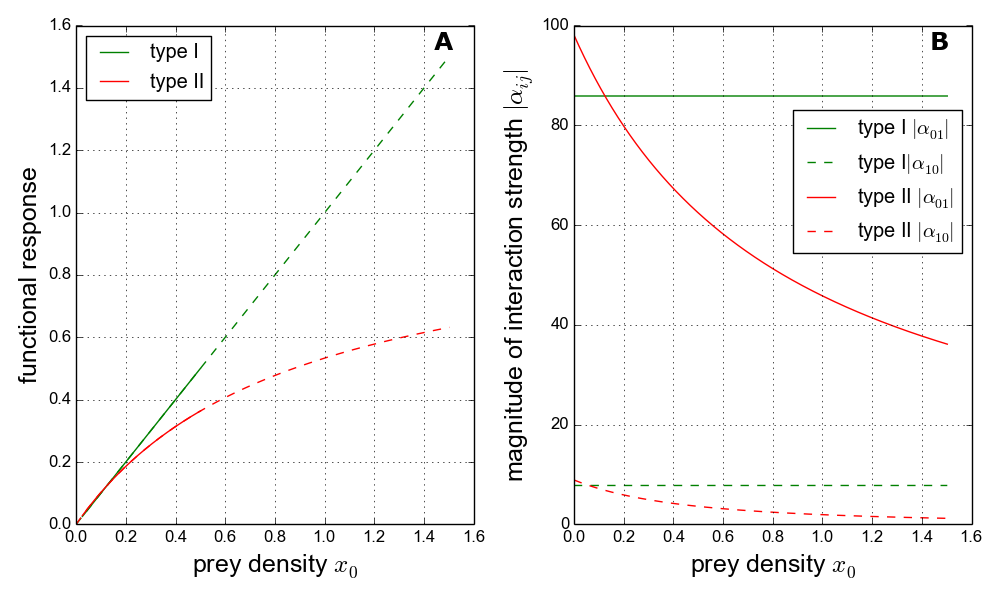
\includegraphics[width=0.8\textwidth]{{{figures/FR_example}}}
\caption[Functional response for \emph{type I} and \emph{type II} models.]{Example of (A) the functional response (FR) curve, and (B) the corresponding inter-specific interaction strengths $\alpha_{ij}$ for one parameter set of the \emph{type I} model (green), and one of the \emph{type II} model (red). The FR for the \emph{type I} model is calculated as $Bx_0$, and for the \emph{type II} model as $Bx_0/(x_0 + D)$. Definitions for $\alpha_{ij}$ in the two models are given in the text. Both parameter sets have values $A=13.58$, $B=85.87$, $7.79$, the \emph{type II} model has $D=0.88$. These parameter values were selected following the procedure described in section \ref{sec:simulation_method}. } 
\label{fig:fr_example}
\end{figure}

Having estimated species interaction strengths using the inference method described above, we compare them to interaction strengths calculated directly from the \emph{data generator}. In doing so we evaluate the performance of the inference method. As discussed in section \ref{sec:intro_interactions} there are numerous metrics available to quantify species interaction strengths. The standard metric to quantify interaction strength from ODE population models is known as the \emph{interaction matrix} $\alpha $ \cite{wootton2005measurement}. This metric allows direct comparison between interaction strengths calculated from different ODE population models. The matrix element $\alpha_{ij}$, quantifies the effect of a small change in the population density of species $j$ on the per capita growth rate of species $i$, and is calculated by

\begin{equation}
\alpha_{ij} = \frac{\partial}{\partial x_{j}}\left(\frac{1}{x_{i}} \frac{dx_i}{dt} \right),
\label{eq:IM}
\end{equation}
%
where $x_i$ and $x_j$ are the population densities of species $i$ and $j$ respectively.  The element $\alpha_{ii}$ quantities an intra-specific interaction such as the density dependent term in the intrinsic growth function \eqref{eq:intrinsic_growth}. Evaluating \eqref{eq:IM} for the GLV model \eqref{eq:glv} gives

\begin{equation}
\alpha_{ij} = J_{ij},
\label{eq:alpha_glv}
\end{equation}
% 
such that the GLV coupling matrix is equal to the interaction matrix for this model. Evaluating \eqref{eq:IM} for the \emph{type I} model (\eqref{eq:lin_mod1} and \eqref{eq:lin_mod2}) gives

\begin{equation}
\alpha_{type\ I} = 
\begin{bmatrix}
-A & -B \\ C & 0
\end{bmatrix}  	,
\end{equation}
%
such that the \emph{type I} model has constant interaction strengths that can be directly compared to those of the GLV model. However evaluating \eqref{eq:IM} for the \emph{type II} model (\eqref{eq:2_mod1} and \eqref{eq:2_mod2}) gives

\begin{equation}\label{eq:im_hii}
\alpha_{type\ II} = 
\begin{bmatrix}
-A + \frac{Bx_1}{(x_0 + D)^2} & \frac{-B}{x_0 + D} \\[10pt] \frac{CD}{(x_0 + D)^2} & 0
\end{bmatrix}  	,
\end{equation}
%
such that the three non-zero interaction strengths are functions of prey density $x_0$, rather than constants. The form of the functional response (FR) curves and inter-specific interaction strengths for the \emph{type I} and \emph{II} models are illustrated in figure \ref{fig:fr_example}. In panel A the non-linearity of the type II FR is visible, modelling the effect of predator saturation as discussed in section \ref{sec:models}. In panel B we see that the result of this non-linearity is interaction strengths that decrease as a function of prey density, whereas the \emph{type I} model has constant interaction strengths. In fact the interaction strengths of the \emph{type II} model tend to zero in the limit that prey density tends to infinity. This property may seem counter intuitive for a measure of interaction strength, since we may expect a large effect of prey on predator when the prey population is very large. Indeed for large prey populations the \emph{biomass} flow does remain large, but the incremental effect of an increase in prey population on the predator growth rate is small.

Based on the comparison of the functional forms in figure \ref{fig:fr_example}, we expect that the ability of a model with constant interaction strengths (such as the GLV model) to approximate the dynamics of the \emph{type II} model may depend on the extent to which the FR deviates from linearity. This hypothesis is investigated in section \ref{sec:res_hii}.

\subsection{Summary of methodology}
\label{sec:method_summary}

Here we summarise the methodology which is depicted in figure \ref{fig:method_flow} and detailed in the sections above. First ODE models (section \ref{sec:models}) are used to simulate population dynamics. This step represents the \emph{data generator}. The population dynamics are then sampled discretely to produce a \emph{data stream}, to which the GLV model (section \ref{sec:def_GLV}) is fitted using the method described in section \ref{sec:timme}. The GLV fit produces constant numeric estimates of interaction strengths in the form of $\hat{J}$, the fitted coupling matrix. Also produced are estimates of the intrinsic growth rate parameters $\hat{r}_i$ for each species. The fitted parameters are compared to those calculated analytically from the \emph{data generator}. The main focus of the analysis is on the estimates of interaction strength given by $\hat{J}$. In particular we are interested in whether $\hat{J}$ correctly identifies the types of interaction between species (i.e. which species eats which), and if so, how accurate are the estimated strengths of the interactions. A secondary concern is the accuracy of the estimated intrinsic growth rates $\hat{r}_i$. However this is related to the main question since the accuracy of all estimates is broadly determined by the \emph{quality} of the GLV fit to the \emph{data stream}.

%The intrinsic growth rates may be compared directly, while the coupling matrix is compared to the interaction matrix $\alpha$ (section \ref{sec:interaction_strength}). 

% The shape of these interaction functions is shown in figure \ref{fig:fr_example}, and we will return to them in section \ref{sec:method_examples}.
%Using the IM we are able to calculate the interaction strengths exactly from the models that we use for simulation. This is because they are ODE models with explicit expressions for $dx_i / dt$, so we can evaluate the partial derivative in equation \eqref{eq:IM} to obtain analytic forms for all the IM elements ($\alpha_{00}$, $\alpha_{01}$, $\alpha_{10}$,$\alpha_{11}$). Depending on the model used the IM elements are either constants, or are functions of prey density. The interaction strengths for our simulation models are given at the end of section \ref{sec:models}, and are illustrated in figure \ref{fig:fr_example}.



\section{Results: ODE as data generator}
\label{sec:results}

In this section we analyse the performance of the inference method (sections \ref{sec:def_GLV} and \ref{sec:timme}) in estimating interaction strengths from noisy two species predator-prey dynamics. The dynamics are simulated using the \emph{type I} and \emph{type II} ODE models (section \ref{sec:models}). In section \ref{sec:noise} we discuss how noise is modelled, and in section \ref{sec:simulation_method} the procedure for numerical simulation of the ODE models is given. Constraints on the parameter values used for simulations are detailed in section \ref{sec:param_selection}. Sections \ref{sec:res_glv} and \ref{sec:res_hii} present results for the \emph{type I} and \emph{type II} models respectively. Both sections analyse the effects of noise and sampling intensity on the accuracy of estimated interaction strengths. In section \ref{sec:res_range_sampling} the impact of non-linearity in the functional response of the predator (a feature of the \emph{type II} model) is studied directly. We quantify the extent of this non-linearity and the effect that it has on the accuracy of results. A novel method for dealing with the non-linearity, referred to as \emph{range sampling}, is also introduced. The focus of this section is on two species systems. In section \ref{sec:ibm} the analysis is extended to systems with more species.

\subsection{Modelling noise}
\label{sec:noise}

A key feature of the simulations is the inclusion of \emph{noise}. Random effects are ubiquitous in natural systems and in ecological data. Therefore in developing a methodology to estimate species interaction strengths it is necessary to characterise its performance under noisy conditions. In modelling population dynamics it is common to distinguish between two different types of error: \emph{process} and \emph{observation} error \cite{hastings2012encyclopedia,jost2000identifying}. Process error results from randomness that is inherent to the mechanisms of the system itself. For example the IBM model used previously (section\ref{sec:the_model}) has randomness built into the behaviour of the individuals. Similarly a natural ecosystem is subject to demographic stochasticity resulting from numerous sources (e.g. environmental forcing, disease etc.). Observation error results from imperfect knowledge of the system being studied. Empirical sampling cannot exactly measure the state of a natural system and therefore some level of observation error is inevitable. In the current analysis we \emph{restrict the focus to process error}, since this type of error is inherent to the system being studied and therefore cannot be reduced. Observation error, on the other hand, may be reduced by experimental design. Therefore we argue that consideration of process error is more important for the development of the methodology presented in this chapter. The exclusion of observation error is also consistent with all previous analyses of the IBM, in which exact knowledge of the system state at any given time point was assumed. Therefore treatment of observation error represents an extension to this work that lies beyond the scope of the current thesis.

In population biology it is conventional to model process error using \emph{multiplicative noise} \cite{carpenter1994fitting,jost2000identifying}. One reason for this is the \emph{postulate of parenthood} (coined by Hutchinson \cite{hutchinson1978introduction}), which states that the growth rate of a species must be equal to zero when the population size is zero. Multiplicative noise is so-name because it consists of a random variable multiplied by the population size $x_i$, such that the term vanishes for zero populations as required by the postulate of parenthood. It is worth noting that the postulate only pertains to \emph{closed-systems}, where there is no external source of individuals (see section \ref{sec:ibm}). Based on convention \cite{jost2000identifying} we define a multiplicative noise term

\begin{equation}
\xi_{i,t} = x_{i,t} \epsilon_{i,t},
\label{eq:mult_noise}
\end{equation}
%
where $\epsilon_{i,t}$ is a random number drawn from a normal distribution with mean zero and variance $\sigma_{noise}\Delta t$. The value $\sigma_{noise}$ is hereafter referred to as the \emph{noise intensity}, and the value $\Delta t$ is the size of the integration time-step used in numerical simulation of the ODE models (see section \ref{sec:simulation_method}). For simplicity we use the same value of noise intensity for both species, although it is possible to define different noise distributions for each species in the system.

\subsection{Simulation procedure}
\label{sec:simulation_method}

%Simulation procedure, parameter selection, additive noise. And plots: example dynamics.
Simulations were run following a standard procedure that ensures consistency and allows comparison between numerical results. All simulations were run using the first-order forward Euler approximation to the deterministic ODE models. It was heuristically determined that this simple approximation produced solutions that were numerically stable for all of the two species systems simulated in this section. The Euler approximation may be defined by the stochastic difference equation

\begin{equation}
\label{eq:stochastic_diff}
x_{i, t+1} = x_{i, t} + \Delta t f(X_t) + \xi_{i,t},
\end{equation}
%
where $x_{i,t}$ is the population density of species $i$ at time $t$; $\Delta t$ is the integration time step; $\xi_{i,t}$ is the noise term \eqref{eq:mult_noise}; and $f_i(X_t)$ defines the time-derivative of $x_{i,t}$ as a function of the system state $X_t \in \mathbb{R}^N$. As such $f_i(X_t) = \dot{x}_i$, which is given by equations (\eqref{eq:1lin_mod1},\eqref{eq:1lin_mod2}) and (\eqref{eq:2_mod1},\eqref{eq:2_mod2}) for the \emph{type I} and \emph{type II} models respectively.

All simulations used the initial condition $x_{i,0} = x_i^*/2 \quad \forall i$, where $x_i^*$ is the equilibrium population level of species $i$ (defined in section \ref{sec:models} for both models. As such the initial system state was consistently away form the equilibrium value. In the event of a stochastic extinction of either species, both population densities were reset to their initial conditions. The case with zero noise intensity ($\sigma_{noise} = 0$) is referred to as the \emph{deterministic case}. In all of the results presented below the simulations were run with a time step $\Delta t = 10^{-4}$. All code was implemented in the language \emph{Python} \cite{python}, and large computations were performed on the cluster \emph{Blue Crystal} \cite{BC3}.

%Key to the experimental approach is the control of certain variables between simulations; the choice of parameter values for the two models; and the introduction of \emph{noise} to the \emph{data generator}. The latter is of particular importance because we are interested in how the possibility of estimating species interaction strengths from population dynamics is hampered by the presence of stochastic effects, which are ubiquitous in natural systems.   
%% note we are noew referring to linear and holling simulation models..
%We apply a strict recipe when running simulations in order to ensure consistency and to allow comparison of our numerical results. Key to this is the control of certain variables across simulations, and also our method for parameter selection, both of which are discussed below. 

\subsection{Parameter selection}
\label{sec:param_selection}

Certain constraints are placed on the parameter values that may be chosen when simulating either ODE model. Two requirements for ecological realism are that the equilibrium populations given by the model are strictly positive, and that this equilibrium is stable. The conditions for the first requirement were given in section \ref{sec:models} as $C>1$ and $C-D>1$ for the \emph{type I} and \emph{type II} models respectively. The conditions for the second requirement are determined from the Jacobian of the model, given by \eqref{eq:jac1} and \eqref{eq:jac2} for the \emph{type I} and \emph{type II} models respectively. If the eigenvalues of the Jacobian have negative real parts then the equilibrium population is locally stable. A further requirement, due to the methodology, is that the simulated dynamics contain sufficient information to fit the GLV model. If the species populations relax to the stable equilibrium too rapidly then it may not be possible to fit the model. To avoid such a problem parameters are chosen such that the deterministic solution to the model is oscillatory (see condition 1 below). Following the precedent of Jost and Arditi (from their paper \cite{jost2000identifying} discussed in section \ref{sec:motivate_interactions}) we stipulate that the deterministic trajectory given by any parameter set must complete \emph{at least} two large amplitude oscillations en route to equilibrium (see condition 2 below). As stated in section \ref{sec:simulation_method}, every simulation is run with the initial population densities set to half of their equilibrium value. This ensures that the system always starts away from equilibrium.
%The goal of fitting the GLV model to simulated population dynamics requires that the dynamics contain enough information to perform the fit - it is not possible to fit the a model if species populations are sitting at equilibrium. Therefore we follow the precedent set in [REF], such that all simulated dynamics of the \emph{deterministic models} exhibit two `large amplitude ' oscillations about a stable equilibrium (see condition 2 below). 

\begin{center}
\begin{table}
\centering
    \begin{tabular}{| l | l | l | l | l |}

    \hline
     & A & B & C & D\\ \hline
    \emph{type I} & 0.1 - 100 & 0.1 - 100 & 1 - 100 & N/A \\ \hline
    \emph{type II} & 0.1 - 100 & 0.1 - 100 & 1.1 - 100 & 0.1-99 \\
    \hline
    \end{tabular}
\caption[Parameter ranges for \emph{type I} and \emph{type II} models.]{Ranges from which parameters were selected uniformly at random for the two ODE simulation models. The parameters are all allowed to vary over at least three orders of magnitude, to ensure that our investigation covers a large region of parameter space. The restrictions on parameters C and D ensure that it is always possible to achieve an equilibrium population of both species that is strictly positive.}
\label{table:p_range}    
\end{table}
\end{center}

Parameters are selected uniformly at random from predefined ranges, which are given in table \ref{table:p_range} for both models. These ranges allow parameter values to vary over at least three orders of magnitude so that our numerical investigation covers a large region of parameter space. Also these ranges ensure that it is possible to select from these ranges a combination of parameter values that produces a positive equilibrium population. If the equilibrium for the selected parameters is positive, then the values are accepted providing they met the following three conditions:
 
\begin{enumerate}
	\item The equilibrium is a locally stable spiral node: the eigenvalues of the Jacobian have negative real parts, and complex conjugate imaginary parts.
	\item The deterministic dynamics exhibit at least two full rotations in the phase plane before relaxing to within $5\%$ of the equilibrium: the distance of the trajectory from the equilibrium as a percentage of the distance of the equilibrium from the origin of the phase plane.
	\item The population densities do not differ by more than an order of magnitude in the deterministic case dynamics.
\end{enumerate}
%
The final conditions helps to avoid the choice of parameters which produce numerical instability in the Euler method, since such numerical instability often leads to divergent population sizes. Using the procedure described above we select a set 100 parameter values for each of the ODE models. Parameter values from these two sets are used to generate all results presented in section \ref{sec:results}. Every simulation, including those with $\sigma_{noise} \neq 0$, is run for the length of time $T_{2P}$ required to achieve two full oscillations (in the deterministic case) for that parameter set.

\subsection{Example dynamics}
\label{sec:method_examples}

\begin{figure}
\centering 
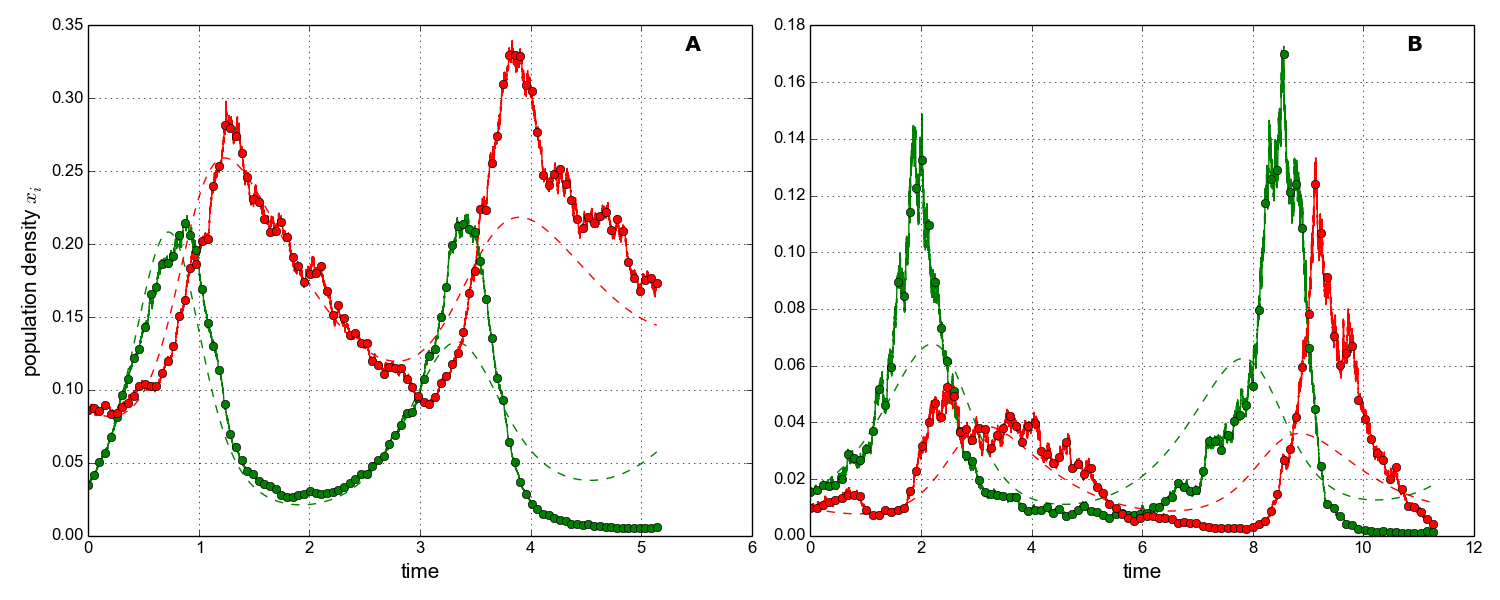
\includegraphics[width=\textwidth]{{{figures/example_dynamics_pID_0_and_87_noise_20.000000}}}
\caption[Dynamics of the \emph{type I} model.]{\textbf{Example dynamics of the \emph{type I} model}. Panels A and B show different parameter sets. Green represents the prey species, and red the predator. The dashed lines show the deterministic trajectories ($\sigma_{noise}=0$); the solid lines show a stochastic trajectory with A: $\sigma_{noise}=20$ and B: $\sigma_{noise}=50$. The solid circles represent the \emph{data stream} of 100 samples, taken from the stochastic dynamics in each case.} 
\label{fig:ex_dynamics_linear}
\end{figure}

%% include here an example of both Linear and HII dynamics (with mean interaction strength), and to demonstrate noise levels. And the results that we get from tinference. And an examples of range samplig (refer forwards to dsicusssion) 
Figure \ref{fig:ex_dynamics_linear} shows examples of dynamics simulated for the \emph{type I} model, with and without noise. Two parameter sets are illustrated, one in each panel. It is clear that the deterministic trajectory completes two full oscillations within the simulation time. The figure also gives an intuition for different levels of noise intensity $\sigma{noise}$. Panel A shows a stochastic trajectory with noise intensity 20, whereas in panel B the noise intensity is 50. In the latter case the noise causes significant deviations from the deterministic trajectories. The peaks in the stochastic prey dynamics are more than double the peaks of the deterministic case. However in both cases depicted the period of oscillation is not significantly altered by noise, which is not necessarily the case in general.

Figure \ref{fig:ex_dynamics_holling} shows examples of dynamics simulated for the \emph{type II} model, and the corresponding time series of the inter-specific interaction strengths $\alpha_{01}$ and $\alpha_{10}$ given by \eqref{eq:im_hii}. The stochastic dynamics illustrated in panels A and C both use $\sigma_{noise}=20$. These dynamics demonstrate that for some parameter sets the trajectories may be more sensitive to the addition of noise than for others. We also see, from panels B and D, that for the \emph{type II} model interaction strengths vary over the course of the simulation (in response to changes in $x_0$). However the extent of this temporal variation in $\alpha_{01}$ and $\alpha_{10}$ is again parameter dependent. The black solid and dashed lines in panels B and D represent the mean values of $\alpha_{01}$ and $\alpha_{10}$ respectively, over the course of the simulations. When fitting the GLV to the \emph{type II} models the estimates interaction strengths $\hat{J}_{ij}$ are compared to these \emph{average values}.


%\clearpage
%\afterpage{%
\thispagestyle{empty}
\begin{sidewaysfigure}

		\centering      
		\hspace{-3cm}

        %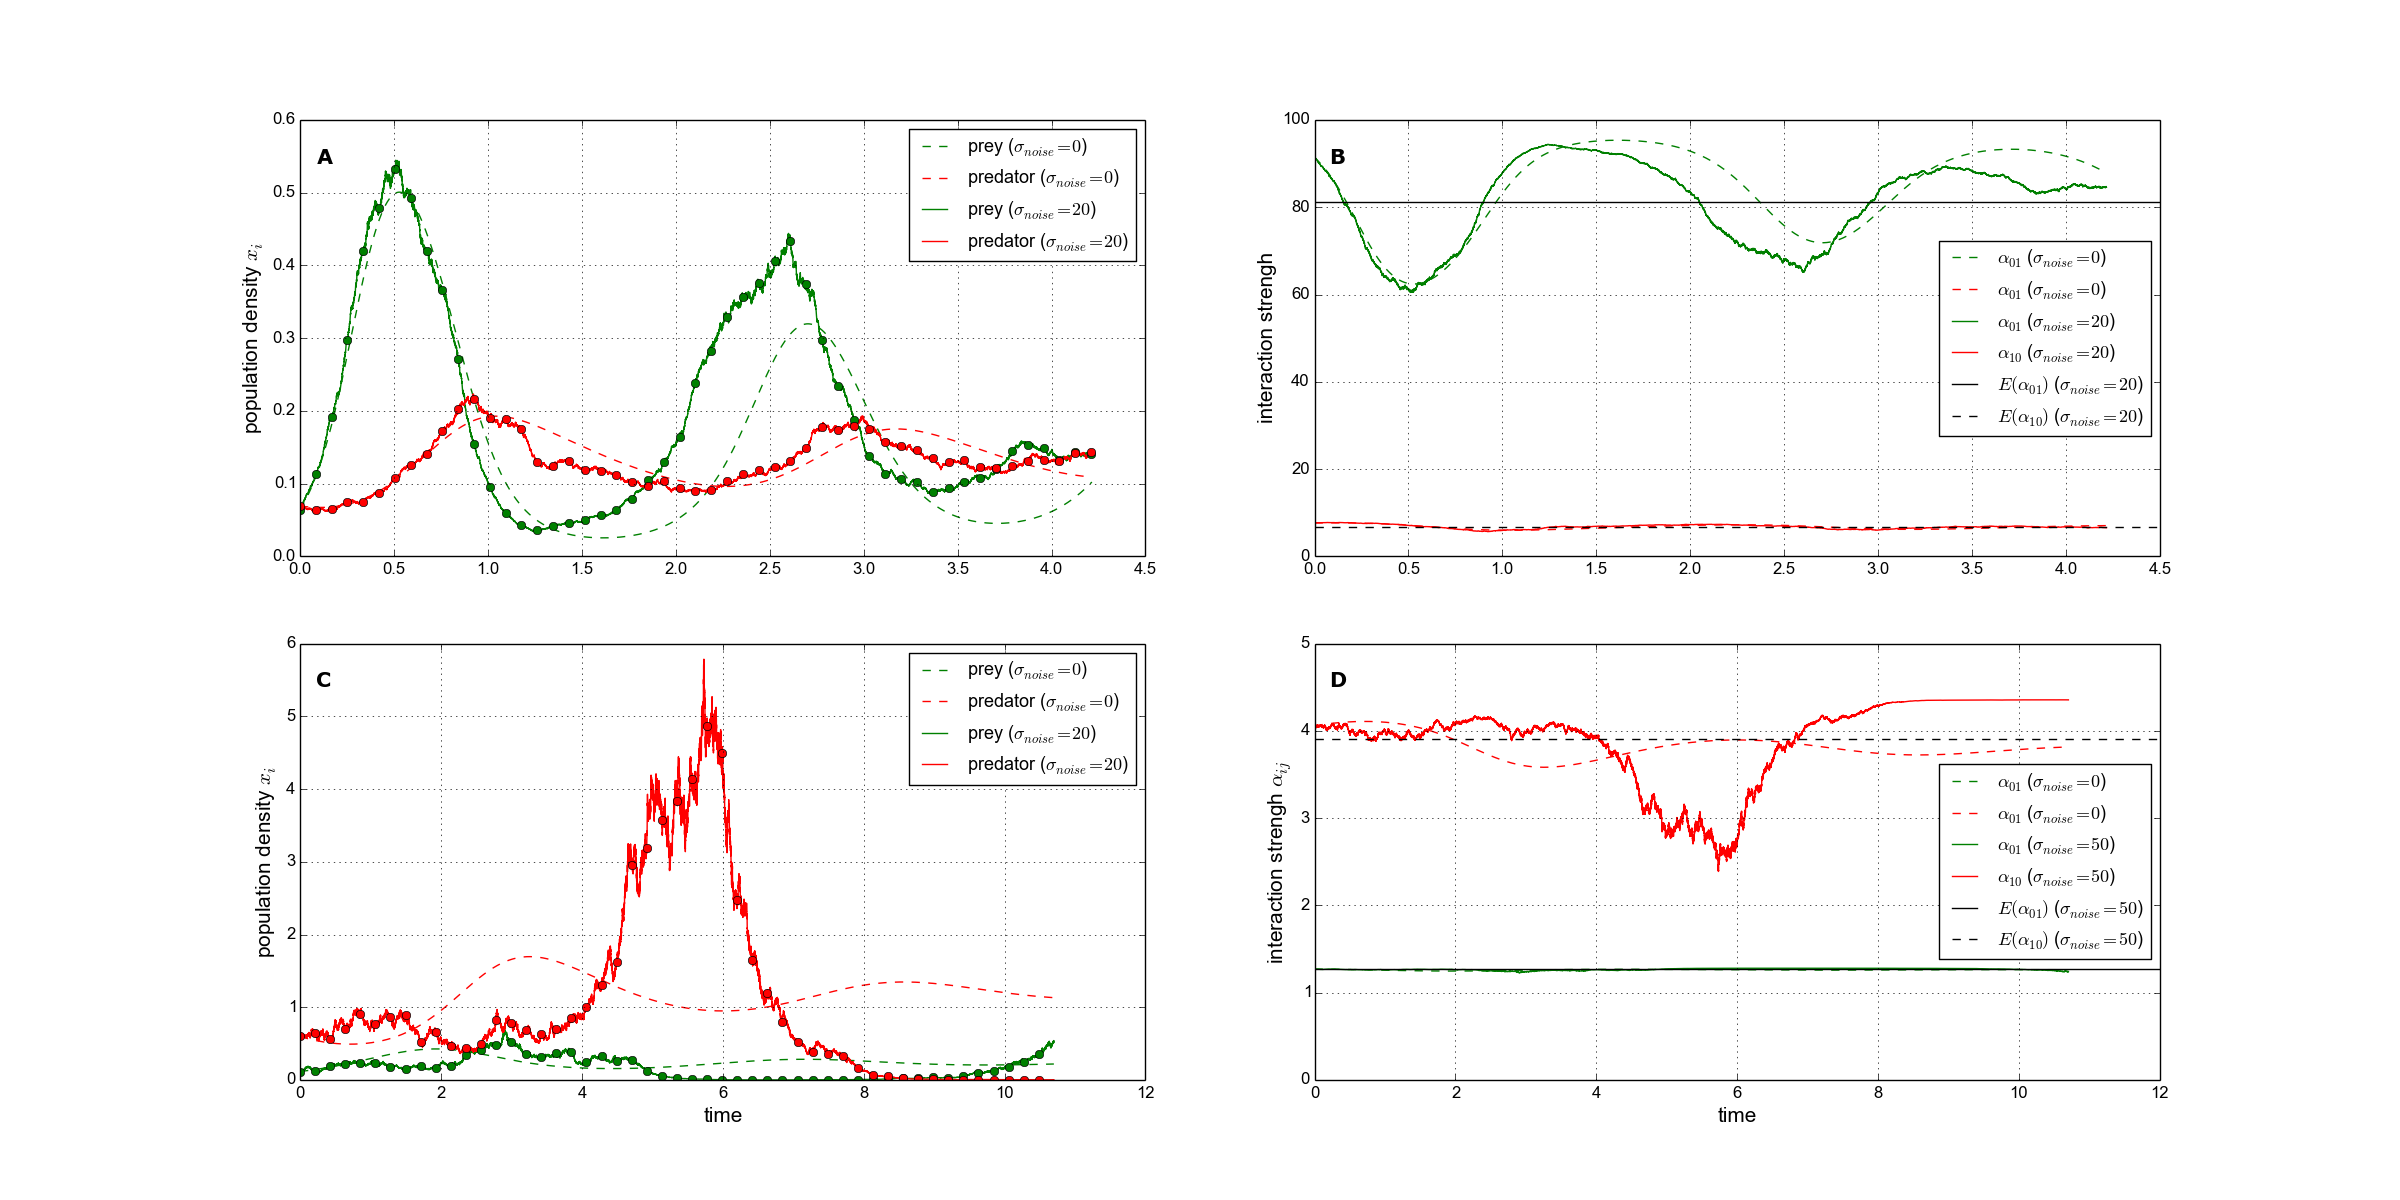
\includegraphics[width=\linewidth]{{{figures/example_dynamics_HII_pID_7_and_0}}}
		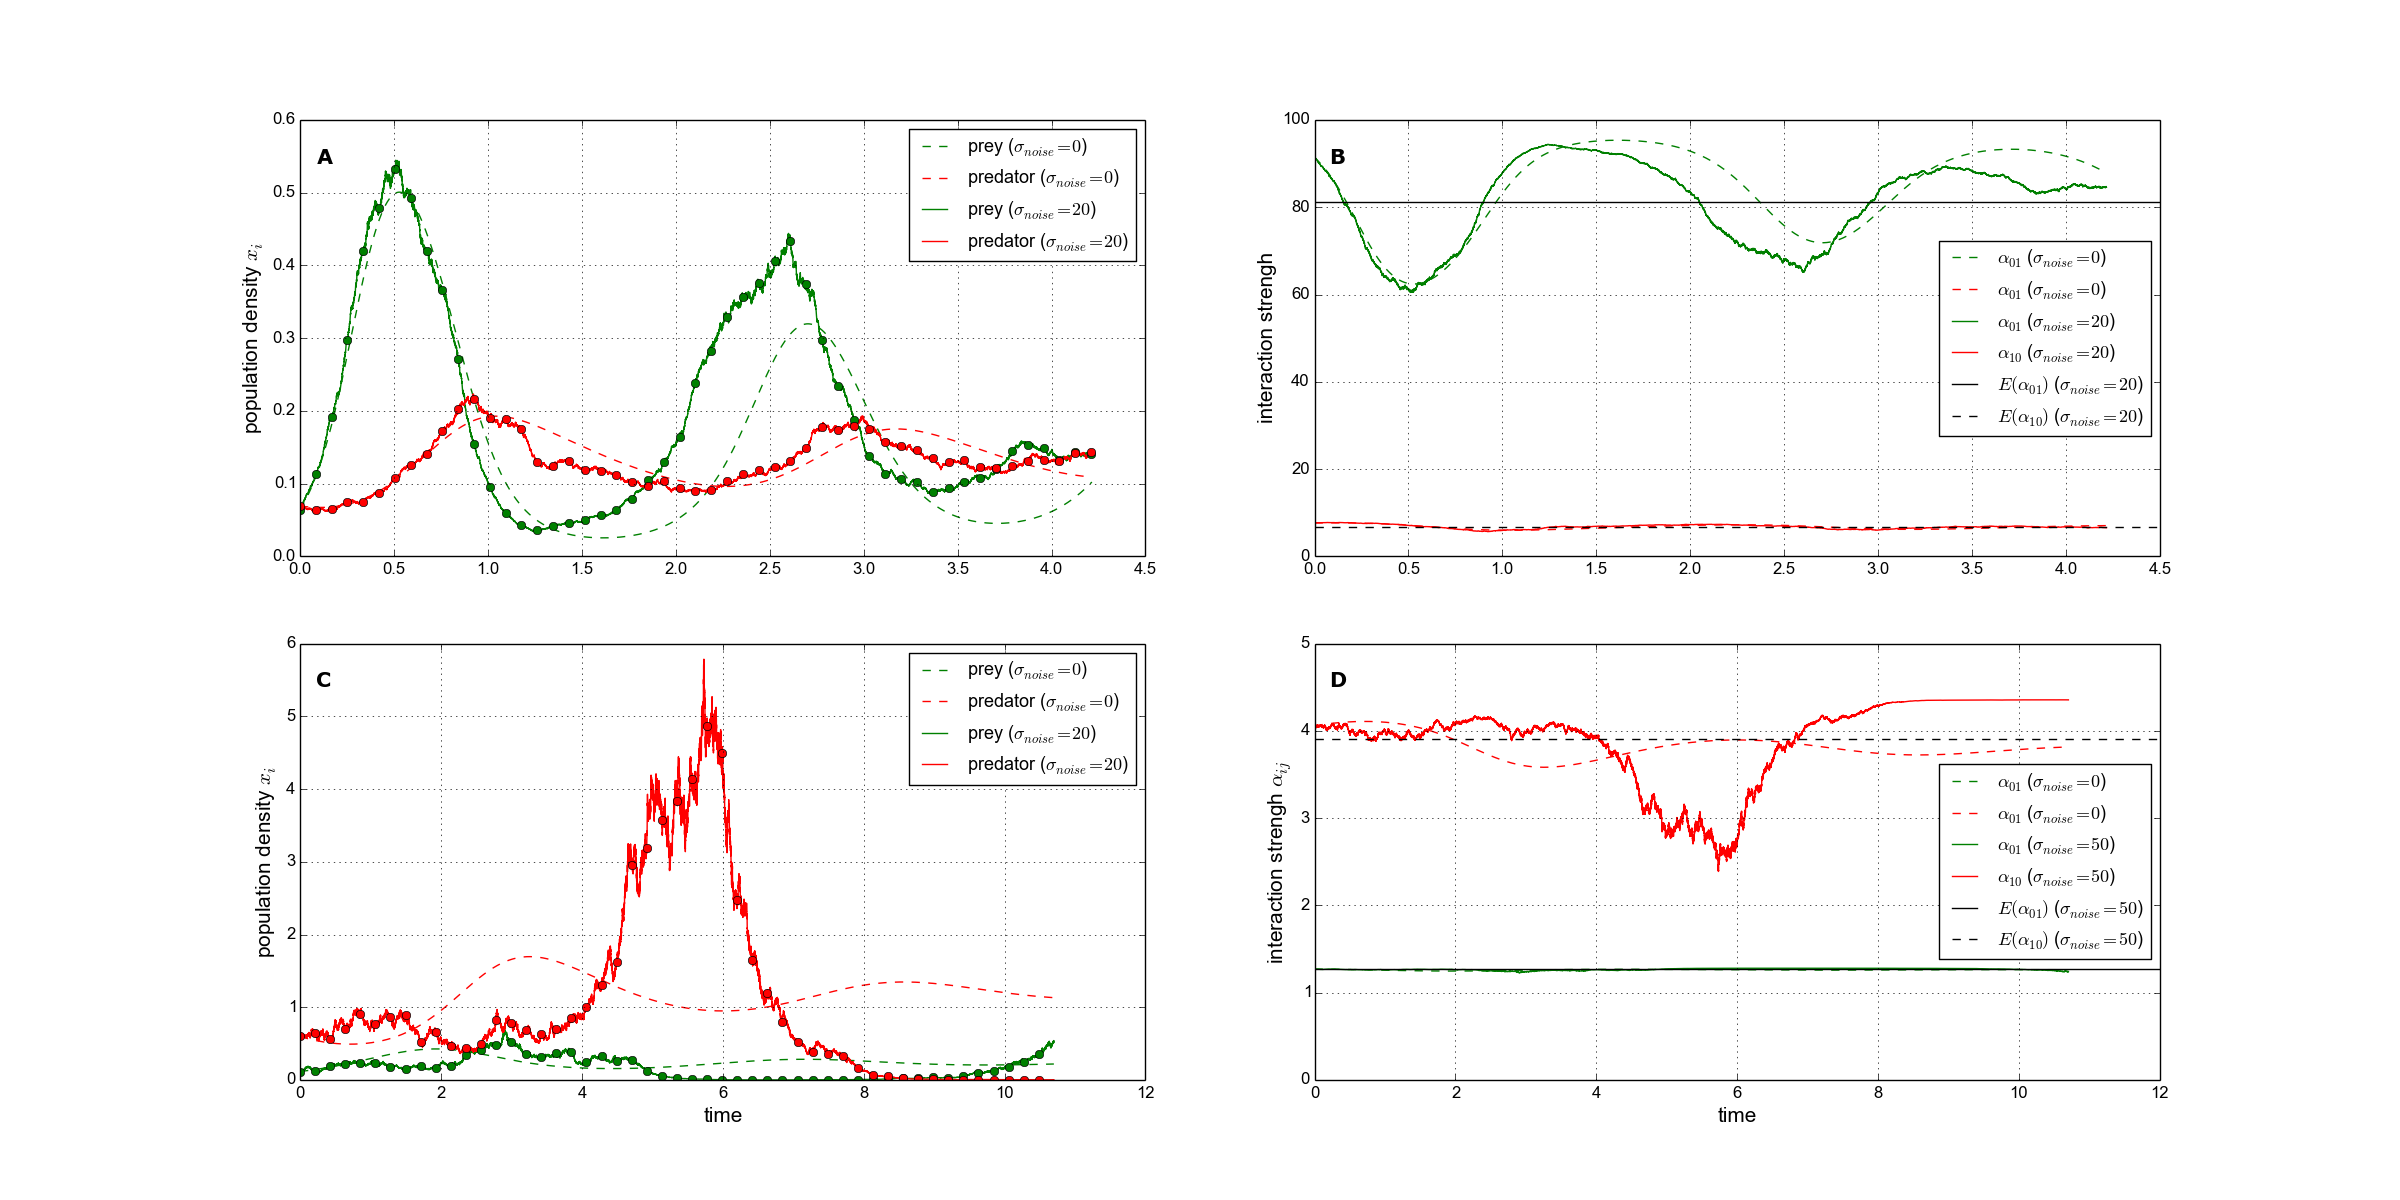
\includegraphics[width=\textwidth]{{{figures/example_dynamics_HII_pID_7_and_0}}}
        \caption[Dynamics of the \emph{type II} model.]{\textbf{Example dynamics and interaction strengths of the \emph{type II} model}. The top and bottom rows show different parameter sets. Green represents the prey species, and red the predator. The dynamics is plotted in panels A and C, using the same format as the \emph{type I} dynamics in figure \ref{fig:ex_dynamics_linear}. In both cases $\sigma_{noise}=20$. Panels B and D show how inter-specific interaction strengths $\alpha_{ij}$ vary with time, corresponding to the dynamics plotted. The black solid and dashed lines indicate the mean interaction strengths for the deterministic dynamics, as indicated in the legend.}\label{fig:ex_dynamics_holling}
        %% Note: this figure generated by Documents/IM_vs_HL_heatmap/plot_sum_maps.py
\end{sidewaysfigure}
%\clearpage
%}


\subsection{Type I model}
\label{sec:res_glv}

In this section we characterise the performance of the inference method (section \ref{sec:timme}) for the \emph{type I} model. Results are presented that compare the estimated GLV parameters (section \ref{sec:def_GLV}) to those of the simulation model. The accuracy of the estimates is evaluated under different levels of noise intensity ($\sigma_{noise}$), and using \emph{data streams} that contain different numbers of samples. As noted in section \ref{sec:def_GLV}, the \emph{type I} model may be expressed in GLV form. Therefore fitting the GLV to this model should produce `exact' estimates of the parameter values in the deterministic case ($\sigma_{noise}=0$). We anticipate that the accuracy of parameter estimates will be reduced at the noise intensity is increased, or as the number of samples is reduced. The noise intensity is varied between 0 (determinism) and 100 (highly stochastic), such that the dynamics depicted in panels A and B of figure \ref{fig:ex_dynamics_linear} correspond to low and intermediate levels of noise respectively. The lower limit on the number of samples that can be used is four, since the system of equations used in the error minimisation must be overdetermined (see section \ref{sec:timme}). The upper limit on the number of samples is constrained by the resolution of the simulated dynamics, which is in turn determined by $\Delta t$ and $T_{2P}$ (see section \ref{sec:param_selection}). It was determined that the upper limit on the number of samples that could be used with all 100 parameter sets was $10^4$. 

\begin{figure}
\centering 
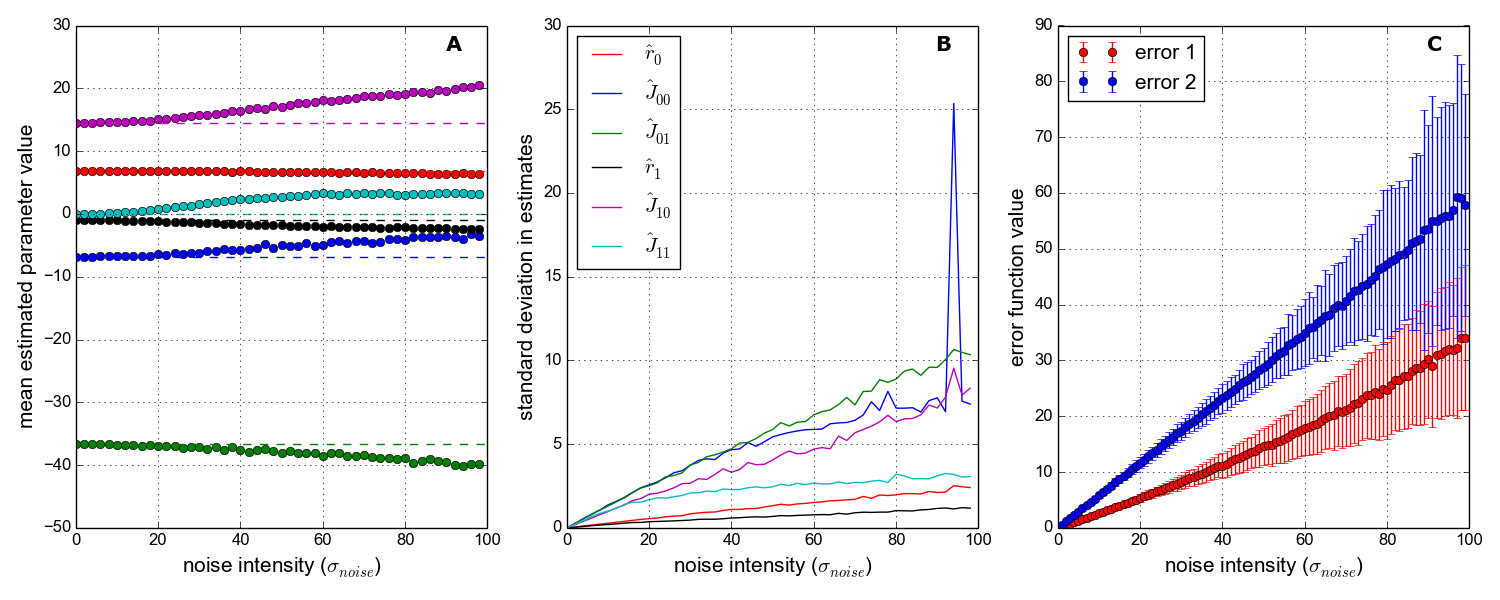
\includegraphics[width=\textwidth]{{{figures/single_params_v_noise_pID_0_nsamples_100}}}
\caption[Effect of noise on parameter estimates for \emph{type I} model.]{\textbf{Effect of noise on parameter estimates for \emph{type I} model}, using a single parameter set. Parameter estimates obtained by fitting GLV model as described in sections \ref{sec:def_GLV} and \ref{sec:timme}. The \emph{data stream} here consists of 100 samples from simulated dynamics, as depicted in figure \ref{fig:ex_dynamics_linear}. Noise intensity is varied between 0 and 100, with 1000 replicate simulations at each noise value. \textbf{Panel A}: Mean estimated parameter values (each dot representing mean over 1000 repeats). The true parameter values of the simulation model (\emph{data generator}) are shown by dashed lines. \textbf{Panel B:} Standard deviation in the parameter estimates. \textbf{Panel C:} Value of the error functions used in the model fitting method (given by \eqref{eq:timme11}), for each species. The circles show the mean error, and the bars show $\pm 1$ standard deviation.} 
\label{fig:sp_v_n_100}
\end{figure}

Figure \ref{fig:sp_v_n_100} shows the effect of increasing noise intensity on parameter estimates, for simulations run using a single parameter set (the same parameter set depicted in panel A, figure \ref{fig:ex_dynamics_linear}). At each value of $\sigma_{noise}$ 1000 replicate simulations were run, and a \emph{data stream} constructed by drawing 100 samples from the simulated dynamics. The GLV model was then fitted to the \emph{data stream}. Panel A shows that, on average, the resulting estimates are close to the true parameter values for low levels of noise. As $\sigma_{noise}$ increases the mean estimated parameter values diverge from the true values. The variability in the parameter estimates, shown in panel B, is zero in the deterministic case, and also increases with noise. It appears that some parameter values  become harder to estimate than others, for this parameter set. For example the estimates of intrinsic growth rate of the prey ($\hat{r}_0$) remain close to the true value, and have relatively low standard deviation, even at the highest noise value ($\sigma_{noise=100}$). Comparatively the estimates of prey intra-specific interaction strength ($\hat{J}_{00}$) perform poorly as noise is increased. Panel C shows the `best-fit' value of the error function \eqref{eq:timme11} for each species, which results from the GLV model fit. The error functions for both species increase approximately linearly with noise. Therefore it is clear that the \emph{quality} of the GLV fit to the simulated dynamics is reduced by noise, as we expected.

\begin{figure}
\centering 
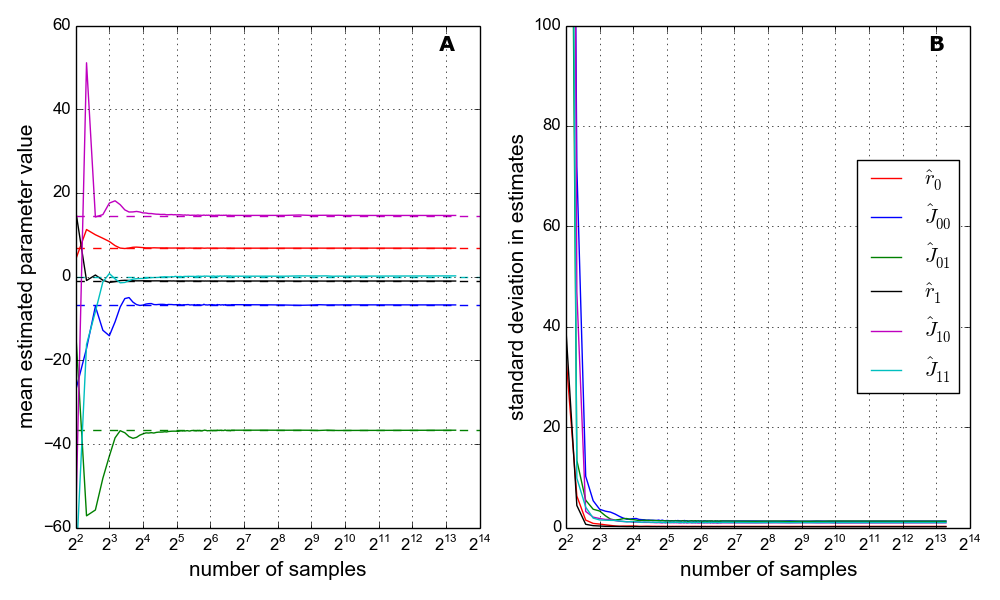
\includegraphics[width=0.67\textwidth]{{{figures/single_params_v_nsamples_pID_0_noise_10.000000}}}
\caption[Effect of the number of samples on parameter estimates for \emph{type I} model.]{\textbf{Effect of the number of samples on parameter estimates for \emph{type I} model}, using the same parameter set as in figure \ref{fig:sp_v_n_100}. Format is similar to that figure, but here 1000 replicate simulations are run at each number of samples, all using $\sigma_{noise}=10$. \textbf{Panel A}: Mean estimated parameter values. The true parameter values of the simulation model (\emph{data generator}) are shown by dashed lines. \textbf{Panel B}: Standard deviation in the parameter estimates.}
\label{fig:sp_v_ns_10}
\end{figure}

Figures \ref{fig:sp_v_ns_10} and \ref{fig:sp_v_ns_50} show the effect of the number of samples on the accuracy of parameter estimates for $\sigma_{noise}=10$ and $\sigma_{noise}=50$ respectively. Both figures show results for the same parameter set as in figure \ref{fig:sp_v_n_100}. In general low numbers of samples ($<10$) produce estimates that are not close to the true values. However as the number of samples is increased the estimates improve. In the low noise case (figure \ref{fig:sp_v_ns_10}) the means of the parameter estimates converge close to the true parameter values (panel A), and  the standard deviations converge to a low but non-zero value. The rate of convergence is such that there appears to be little improvement in parameter estimates for numbers of samples greater than 100. In the intermediate noise case (figure \ref{fig:sp_v_ns_50}) the means of the parameter estimates approximately converge, but not necessarily on the true parameter values. In panel A we see that, even with $10^4$ samples, there are a clear discrepancies between the true and the estimated values of some parameters. Additionally the standard deviations converge (panel B), but on higher values than in figure \ref{fig:sp_v_ns_10} due to the increased level of noise. As in the low noise case there appears to be little improvement in the estimates above 100 samples.
%\footnote{Two key points: even at low noise a single simulation may produce estimates that are slightly off due to the non-zero standard deviation. At higher levels of noise the mean value is also off. We conclude that noise can induce systemative errors in the estimates..}

\begin{figure}
\centering 
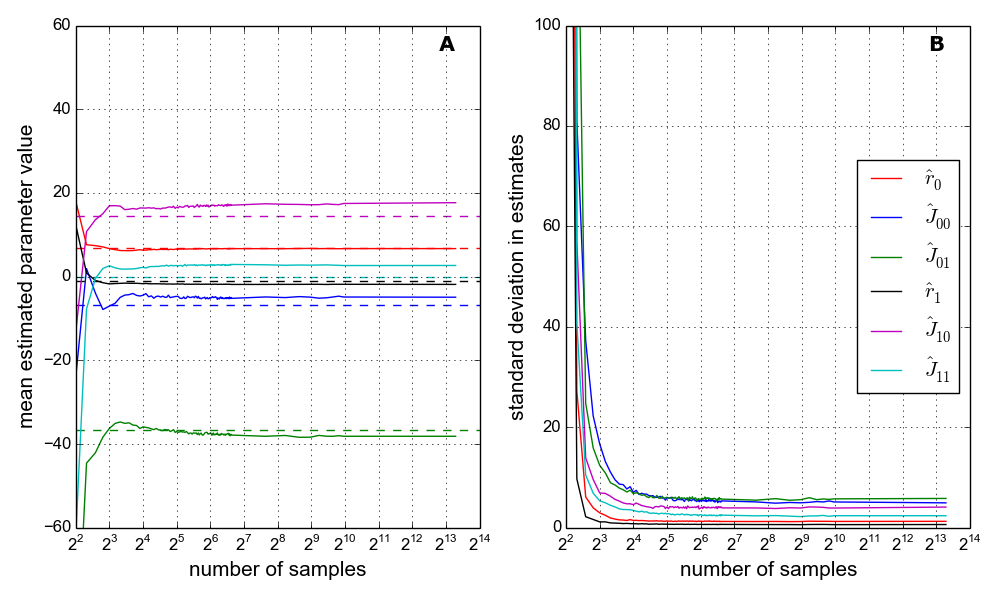
\includegraphics[width=0.67\textwidth]{{{figures/single_params_v_nsamples_pID_0_noise_50.000000}}}
\caption[Effect of the number of samples on parameter estimates for \emph{type I} model, with high noise.]{Similar to figure \ref{fig:sp_v_ns_10} but with noise intensity $\sigma_{noise}=50$.} 
\label{fig:sp_v_ns_50}
\end{figure}

%% Probably not include this figure as its basically the same!!
%\begin{figure}[h]
%\centering 
%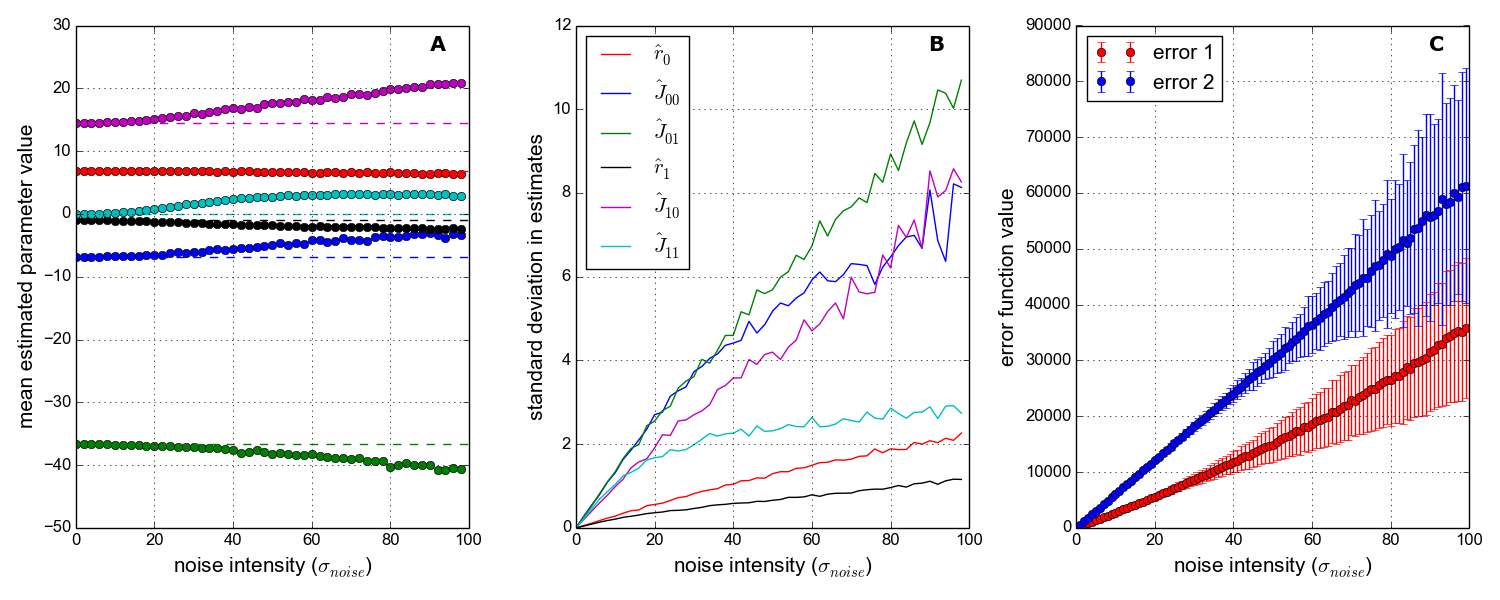
\includegraphics[width=\textwidth]{{{figures/single_params_v_noise_pID_0_nsamples_10000}}}
%\caption{Exactly as in figure \ref{fig:sp_v_n_100} but using 10,000 samples from the simulated dynamics.} 
%\label{fig:sp_v_n_10000}
%\end{figure}

We now generalise the above results by considering an ensemble of 100 parameter sets. To quantify the accuracy of parameter estimates we define a metric for \emph{relative error}:

\begin{equation}
RE(p_i) = \frac{|p_i - \hat{p}_{i}|}{|p_i|},
\label{eq:rel_error_param}
\end{equation}  
%
where $p_i$ and $\hat{p}_i$ are the true and estimated value of parameter $i$ respectively. As such $RE$ is equal to zero if the estimated and true value are equal. This metric may be evaluated for any of the model parameters (unless $p_i=0$). In the analysis that follows we focus on the inter-specific interaction strengths $J_{01}$ and $J_{10}$, since quantification of these is the main motivation for the work. Also, as suggested by figures \ref{fig:sp_v_n_100}-\ref{fig:sp_v_ns_50}, the error in these parameters may be used as a proxy for the quality of the model fit as a whole. 

Figures \ref{fig:ep_v_n} and \ref{fig:ep_v_ns} show the effect of noise and number of samples on the relative errors $RE(J_{01})$ and $RE(J_{10})$. At each value of noise intensity, and for each number of samples, 100 replicate simulations were run for each of the 100 parameter sets. The mean and standard deviations of the $RE$ metric over these 10,000 simulations, are plotted in panels A and B of both figures. From figure \ref{fig:ep_v_n} we observe the general feature that both the mean and the variability of the error increase with noise intensity. Figure \ref{fig:ep_v_ns} shows that both the mean and the variability of the error are reduced by increasing the number of samples. In this case $\sigma_{noise}=50$, and as a result the mean relative error does not converge to zero (panel A). This is consistent with our results derived from a single parameter set.

\begin{figure}
\centering 
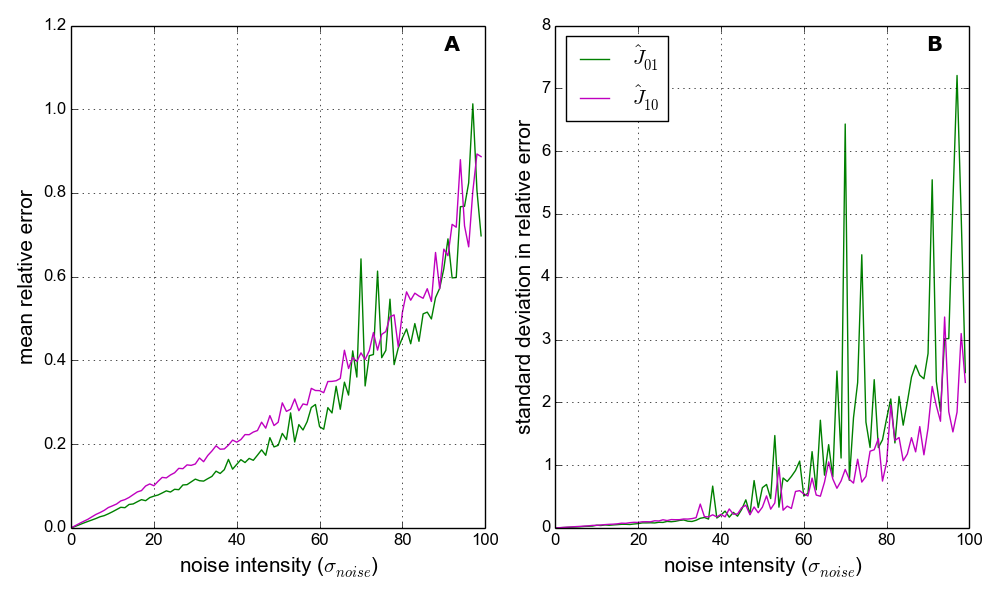
\includegraphics[width=0.67\textwidth]{{{figures/ensemble_params_vs_noise_nsamples_1000}}}
\caption[Effect of noise on parameter estimates, ensemble of 100 simulations of \emph{type I} model.]{\textbf{Effect of noise on parameter estimates for \emph{type I} model}, over 100 different parameter sets. The \emph{data stream} here consists of 1000 samples. At each value of $\sigma_{noise}$ 100 replicate simulations were run for each of the 100 parameter sets. Results shown are statistics for the full ensemble of simulations. \textbf{Panel A}: Mean relative error (defined in text) in estimates of the two inter-specific interaction strengths ($\hat{J}_{01}$ and $\hat{J}_{10}$). \textbf{Panel B}: Standard deviation in these errors over all replicates.}
\label{fig:ep_v_n}
\end{figure}

\begin{figure}
\centering 
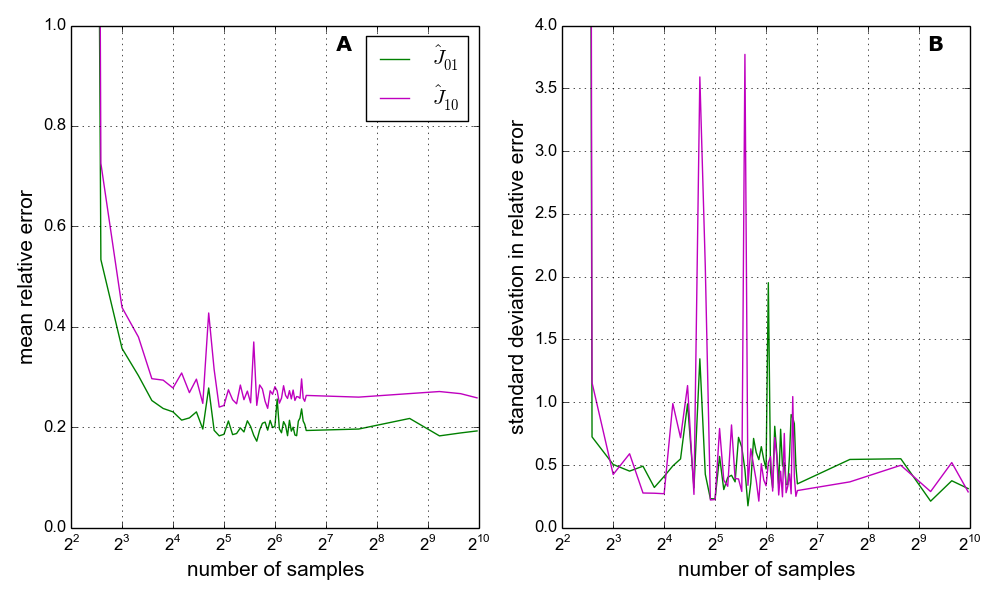
\includegraphics[width=0.67\textwidth]{{{figures/ensemble_params_vs_nsamples_noise_50.000000.IS}}}
\caption[Effect of number of samples on parameter estimates, ensemble of 100 simulations of \emph{type I} model.]{Similar to figure \ref{fig:ep_v_n}, but the relative errors in the estimates are plotted against number of samples. Noise intensity $\sigma_{noise}=50$.}
\label{fig:ep_v_ns}
\end{figure}


\subsection{Type II model}
\label{sec:res_hii}

In this section we conduct a similar analysis of the inference method as in section \ref{sec:res_glv}, but this time using the \emph{type II} model as the \emph{data generator}. As we have seen (for example in figure \ref{fig:ex_dynamics_holling}) the interaction strengths $\alpha_{ij}$ in the \emph{type II} model are not constants. They are functions of prey density $x_0$, and therefore vary over the course of a simulation. In order to draw comparisons with $\hat{J}_{ij}$, the constant numeric estimates of interaction strength produced by the GLV fit, we take the mean values of the $\alpha_{ij}$ over a simulation. In the analysis below we assess whether the GLV estimates of interaction strength are close to these mean values. The intrinsic growth rates of the \emph{type II} model are constant, and therefore may be compared directly to the GLV estimates $\hat{r}_i$.

\begin{figure}
\centering 
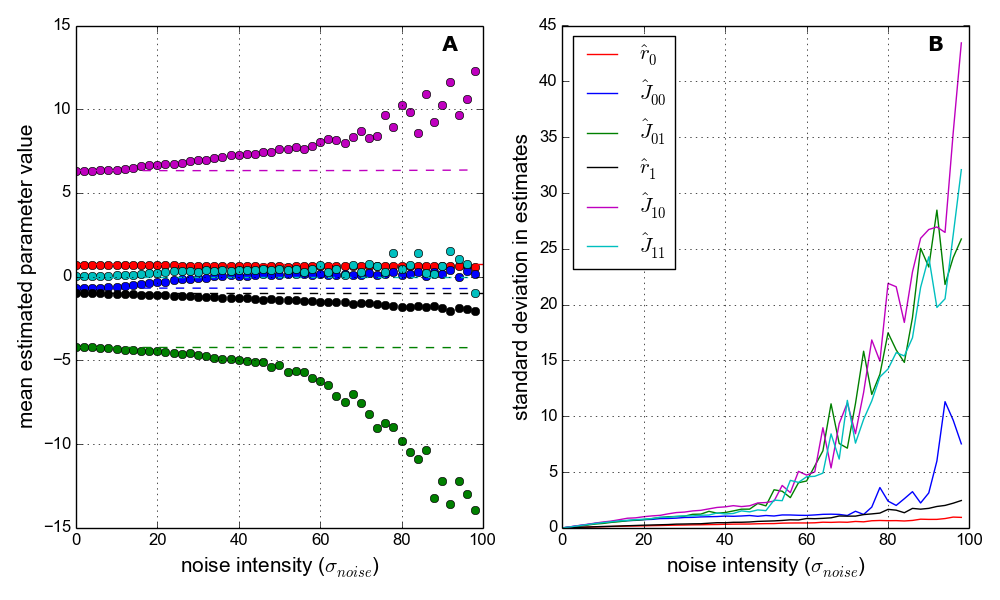
\includegraphics[width=0.67\textwidth]{{{figures/single_params_v_noise_pID_87_nsamples_10000.HII}}}
\caption[Effect of noise on parameter estimates, \emph{type II} model.]{Similar to figure \ref{fig:sp_v_n_100}, but for the \emph{type II} model, and using a \emph{data stream} of 10,000 samples. In this case the simulation interaction strengths $\alpha_{ij}$ are functions of prey density. Therefore the estimates $J_{ij}$ are compared to the mean values of $\alpha_{ij}$, plotted as dashed lines.}
\label{fig:hii_sp_v_n}
\end{figure}

Figure \ref{fig:hii_sp_v_n} show how the GLV estimates respond to increasing levels of noise, for a single parameter set. In general it was found that the estimates of interaction strength were less accurate for the \emph{type II} model than for \emph{type I}. This was expected since the GLV can only approximate the \emph{type II} model, whereas it can exactly represent the \emph{type I}. In an attempt to improve the results, the calculations shown in figure \ref{fig:hii_sp_v_n} use 10,000 samples (whereas those in figure \ref{fig:sp_v_n_100} used 100 samples). To provide a benchmark interaction strength for this parameter set that is consistent across all simulations we use the mean values of the $\alpha_{ij}$ over the deterministic trajectory. These are the values displayed as dashed lines in figure \ref{fig:hii_sp_v_n}. Panel A shows that, for low noise intensities, the GLV parameter estimates are close to those of the \emph{data generator}. As the noise intensity increases the estimates diverge. Comparing figure \ref{fig:hii_sp_v_n} to figure \ref{fig:sp_v_n_100} it appears that the estimates are more sensitive to noise in the \emph{type II} case, despite the use of a larger number of samples. Therefore it appears that, with low levels of noise, the GLV model can well approximate the mean interaction strengths of the \emph{type II} model, as least for this parameter set. However these estimates may become unreliable as the level of noise increases.

\begin{figure}
\centering 
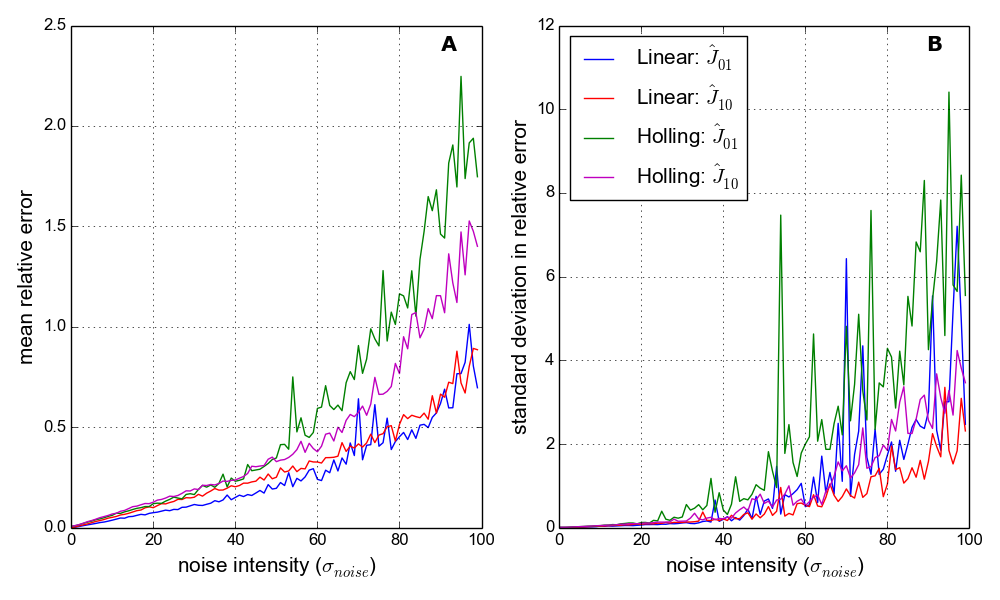
\includegraphics[width=0.67\textwidth]{{{figures/ensemble_params_vs_noise_nsamples_1000.B}}}
\caption[Effect of noise on parameter estimates for both \emph{type I} and \emph{type II} models.]{Similar to figure \ref{fig:ep_v_n}, but showing relative errors for both the \emph{type I} and \emph{type II} models. Number of samples is 1000.}
\label{fig:hii_ep_v_n}
\end{figure}


In order to generalise the analysis over a range of parameter values we again define a metric for \emph{relative error}:

\begin{equation}
RE(p_i) = \frac{|\bar{p}_i - \hat{p}_{i}|}{|\bar{p}_i|},
\label{eq:rel_error_param_II}
\end{equation}  
%
which is the same as for the \emph{type I} relative error, except that $\bar{p}_i$ is the mean value of model parameter $p_i$ over the simulation in question. This allows us to again draw comparisons between the accuracy of estimates obtained from simulations using different parameter values. We conduct the same analysis as for the \emph{type I} model, with 1000 replicates for each of the 100 parameter sets over a range of noise intensities and sample numbers. Figures \ref{fig:hii_ep_v_n} and \ref{fig:hii_ep_v_ns} provide a direct comparison between the relative errors for the \emph{type I} and \emph{type II} models. The errors for both models respond to noise and number of samples in qualitatively the same way. However the mean errors, and often the variability in the errors, are larger for the \emph{type II} than for the \emph{type I} model. For example the mean relative errors for the \emph{type I} model converge on value between about 0.2 and 0.3 for high number of samples, whereas they converge on values between about 0.3 and 0.4 for the \emph{type II} model (figure \ref{fig:hii_ep_v_ns}).

%Conclusion: noise can introduce systematic errors. Larger number of samples required when noise is high. \textbf{Deviation of FR form linearity} - new plots.

%% Note sure this is informative:
%\begin{figure}
%\centering 
%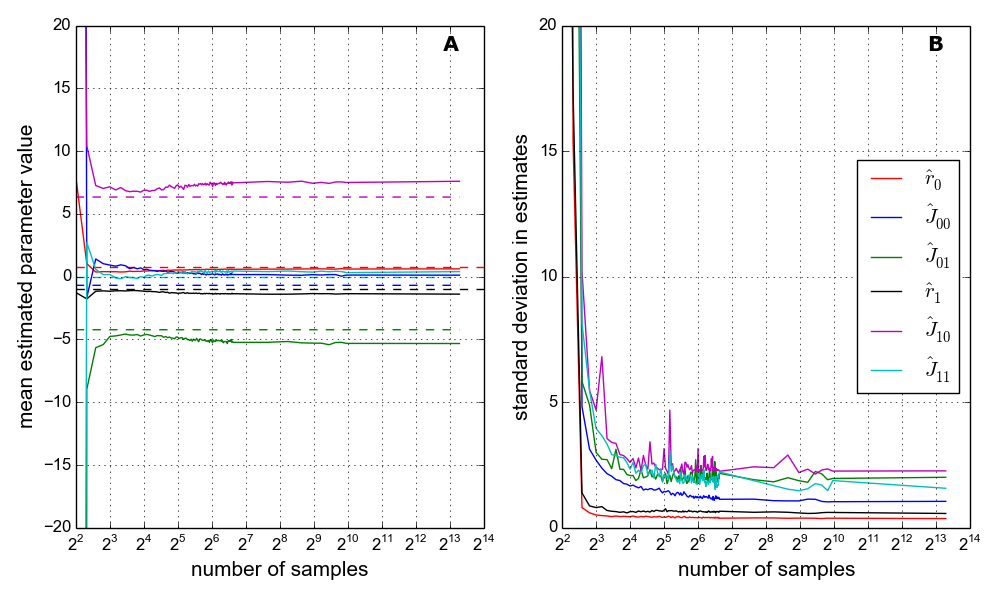
\includegraphics[width=0.67\textwidth]{{{figures/single_params_v_nsamples_pID_87_noise_50.000000.HII}}}
%\caption{Noise is 50.} 
%\label{fig:hii_sp_v_ns}
%\end{figure}

\begin{figure}
\centering 
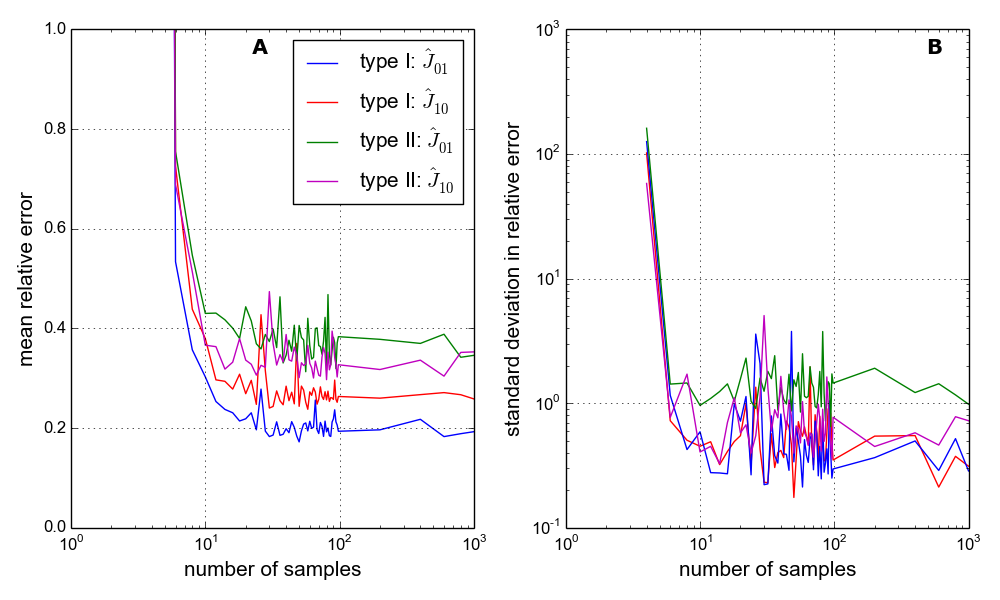
\includegraphics[width=0.67\textwidth]{{{figures/ensemble_params_vs_nsamples_noise_50.000000.B.IS}}}
\caption[Effect of number of samples on parameter estimates for both \emph{type I} and \emph{type II} models.]{Similar to figure \ref{fig:ep_v_ns}, but showing relative errors for both the \emph{type I} and \emph{type II} models. $\sigma_{noise}=50$.} 
\label{fig:hii_ep_v_ns}
\end{figure}


%\subsection{Range sampling}
\subsection{Quantifying non-linearity}
\label{sec:res_range_sampling}

The observation that the errors in the estimates of interaction strength are larger for the \emph{type II} model than for the \emph{type I} is related to the form of the functional response (FR). The \emph{type II} model has a non-linear FR, which results in variable interaction strengths that can only be approximated by the GLV. This leads us to propose that the quality of estimates obtained from the dynamics of the \emph{type II} model may depend on the extent of the non-linearity in the FR. The more linear the FR, the better we expect the GLV approximation to be. In order to test this hypothesis we develop a method for quantifying the extent of the non-linearity in the \emph{type II} FR. This method is depicted in figure \ref{fig:nonlinear_fr_rsq}.

\begin{figure}
	\centering
	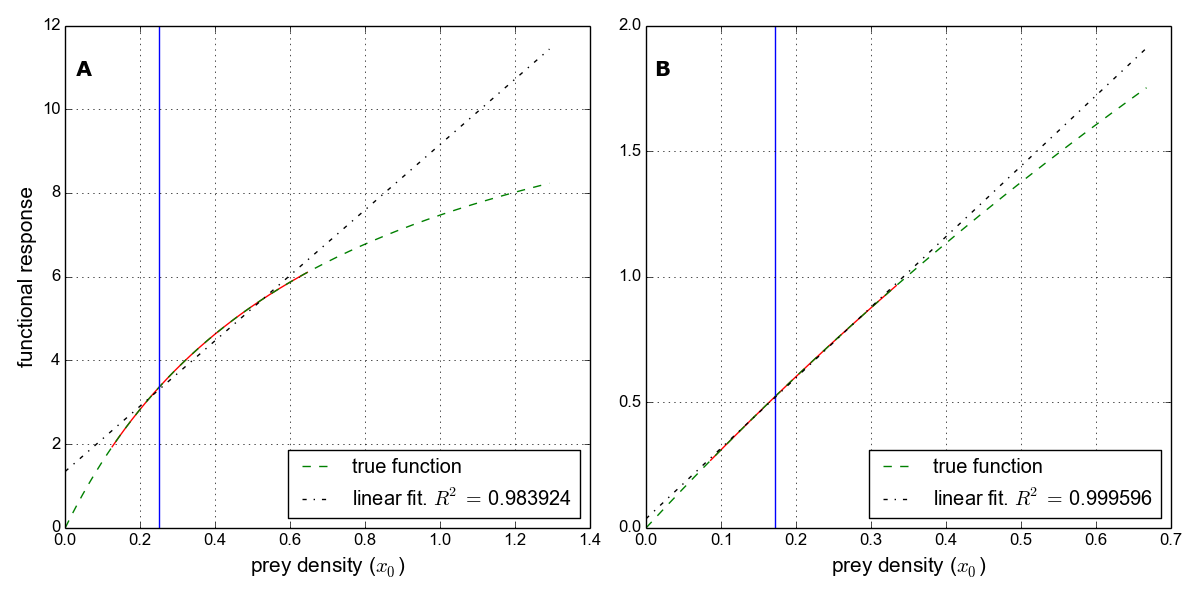
\includegraphics[width=\textwidth]{{{figures/example_FR_linear_nonlinear}}}
	\caption[Non-linear functional response in \emph{type II} model.]{\textbf{The functional response (FR) of the predator} for two different parameter sets. The FRs plotted are given by $Bx_0 / (x_0 + D)$. The green dashed line shows the analytic form of the function, the red line shows the region of the function explored during a deterministic simulation with those parameters. The black dashed line shows a linear regression fit to the explored FR (red line). The $R^2$ value of this fit can be used to quantify how well the FR  is approximated by linearity, in the region explored by the dynamics. The blue vertical line indicates the prey equilibrium population $x_0^*$. \textbf{Panel A}: The least linear (lowest $R^2$) FR from the 100 parameter sets investigated. \textbf{Panel B}: The most linear (highest $R^2$) FR from the same 100 parameter sets.}
	\label{fig:nonlinear_fr_rsq}
\end{figure}

Panels A and B of figure \ref{fig:nonlinear_fr_rsq} show the \emph{type II} FR for two different parameter sets. The FR is defined by $Bx_0 / (x_0 + D)$. The red lines indicate the region of the FR that is explored by the deterministic trajectory when dynamics are simulated with these parameter values. A linear regression model is fitted to this region of the FR, and the $R^2$ value of the fit is to quantify how good the linear approximation is. If the FR were completely linear in this region then the $R^2$ value would be one. The lower the $R^2$ value, the further the deviation of the FR from linearity. Panels A and B show the least and most linear FRs, according to the $R^2$ values, from the 100 parameter sets chosen for the \emph{type II} model (i.e. same parameter sets used to generate figure \ref{fig:hii_ep_v_ns}).

%% These rather confusing!
%%Plotted by: second_year/functional_response_paper/final_code_version/hollingIIFR/many_short_params/FR_nonlinearity.py
%% But using the 100 params with lowest Rsq value, selected from the 1000 params generated on BC3.
%% Both plotted using same script with different plot flags at the end.
\begin{figure}
	\centering
	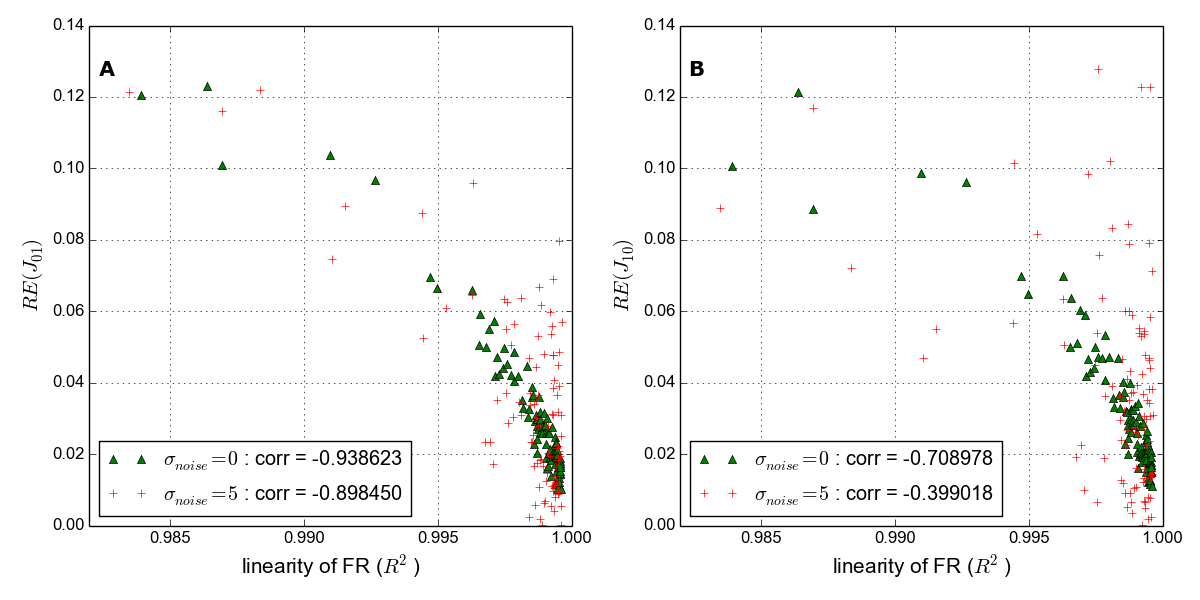
\includegraphics[width=\textwidth]{{{figures/nonlinearity_predicts_quality}}}
	\caption[Linearity of functional response as a predictor for estimate quality.]{\textbf{Linearity of FR as a predictor for estimate quality.} One simulation for each parameter set at each noise value: $\sigma_{noise}=0$ (green triangles), and $\sigma_{noise}=5$ (red crosses). Linearity of the FR is measured by the $R^2$ of the regression fit, as in figure \ref{fig:nonlinear_fr_rsq}. The $R^2$ value is plotted against the relative error (RE) in the estimates of inter-specific interaction strength. The correlation coefficient between the two variables is given in the legends. \textbf{Panel A}: Prey interaction strength $\hat{J}_{01}$, \textbf{Panel B}: Predator interaction strength $\hat{J}_{10}$.}
	\label{fig:nonlinearity_error}
\end{figure}

Using this $R^2$ measure for linearity in the FR, we then investigate the correlation between linearity and the relative error (RE) in the estimates of interaction strength. The same RE metric \eqref{eq:rel_error_param_II} is used to quantify the error in the estimates $\hat{J}_{01}$ and $\hat{J}_{10}$. The relative errors are plotted against $R^2$ for each of the 100 parameter sets in figure \ref{fig:nonlinearity_error}. There are two simulations for each parameter set, one for $\sigma_{noise}=0$ (green triangles) and one for $\sigma_{noise}=5$ (red crosses). In general we observe that the relative error is higher for parameter sets with less linear FR (lower $R^2$), as predicted. The correlation is weakened by noise, especially for the predator interaction strength $J_{10}$. At $\sigma_{noise}=5$ the correlation between $RE(J_{10})$ and $R^2$ is only 0.40, compared to 0.71 at $\sigma_{noise}=0$. This reduction in correlation suggests that, although the linearity of the FR is significant at low (or zero) noise values, the introduction of noise represents a source of error in the estimates which is not dependant on linearity. Indeed the extent to which noise produces error in the estimates is likely to depend on the sensitivity of the dynamics to stochastic perturbations. As we saw in figure \ref{fig:ex_dynamics_holling}, the same level of noise can cause the dynamics to deviate to different extents from the deterministic trajectory, depending on the parameter values. This sensitivity to nosie can be studied analytically using stability concepts such as \emph{reactance} and \emph{resilience} \cite{arnoldi2015}. However we do not pursue this line of investigation here.  

\begin{figure}
	\centering
	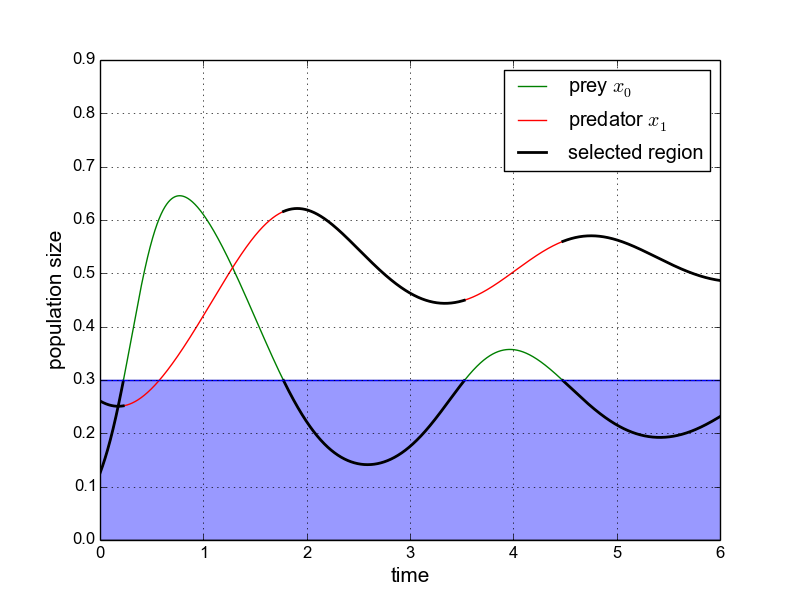
\includegraphics[width=0.6\textwidth]{{{figures/range_sample_didactic}}}
	\caption[Demonstration of range sampling procedure.]{\textbf{Demonstration of range sampling} from dynamics, in order to perform a piece-wise fit of the GLV. The dynamics shown is from the \emph{type II} model. The dynamics is split into two ranges according to prey density $x_0$ such that half of the time points fall into one range and half into the other. The region of prey density that defines the lower range is shaded in blue, and the portions of the dynamics that fall into this range are highlighted in black.}
	\label{fig:range_didact}
\end{figure}
%% These rather confusing!
%%Plotted by: second_year/functional_response_paper/final_code_version/hollingIIFR/many_short_params/range_sample.py
%% But using the least linear of 100 params with lowest Rsq value, selected from the 1000 params generated on BC3.
%% Both plotted using same script with different plot flags at the end.
%% Noise is zero or 5.
\begin{figure}
	\centering
	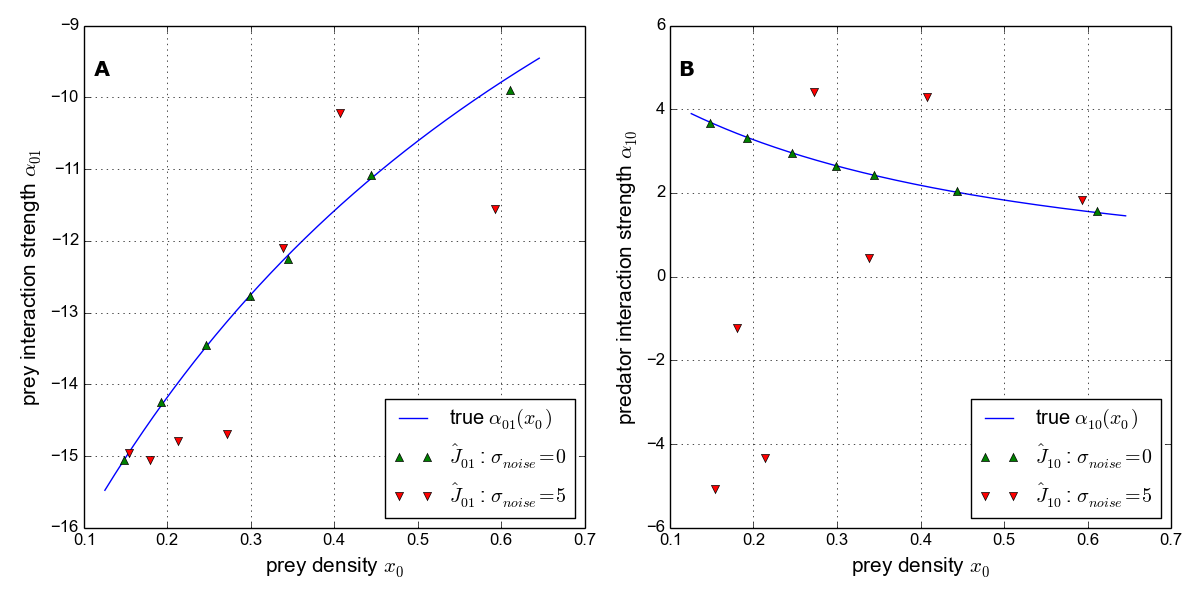
\includegraphics[width=\textwidth]{{{figures/range_sample}}}
	\caption[Range sampling results]{\textbf{Range sampling results} for the parameter set depicted in panel A of figure \ref{fig:nonlinear_fr_rsq}. The dynamics is split into seven ranges using the same procedure illustrated in figure \ref{fig:range_didact}. The GLV is then fitted separately (piece-wise) to these seven ranges, producing estimates of the interaction strength within each range. Results are calculated from single simulations, one with $\sigma_{noise}=0$ (green triangles), and one with $\sigma_{noise}=5$ (red triangles). Also plotted, as a blue line, is the analytic form of the interaction strength calculated from the \emph{type II} model using \eqref{eq:im_hii}. \textbf{Panel A}: Prey interaction strength $\alpha_{01}$, \textbf{Panel B}: Predator interaction strength $\alpha_{10}$.}
	\label{fig:range_example}
\end{figure}

From figure \ref{fig:nonlinearity_error} we observe that most of the parameter sets investigated have FRs that are approximately linear ($R^2$ values close to one) within the region of phase-space explored by the deterministic dynamics. This is an unintended feature of the parameters sets, resulting from the constraints imposed in parameter selection. The approximate linearity of the FR in many cases leads us to question if a signature of non-linearity can be detected using our methodology. Previous work by Jost and Arditi \cite{jost2000identifying} has attempted to detect the presence of different forms of functional response from population dynamics data. Their approach was to fit ODE models with different forms of FR, selecting the model that produced the `best fit'. As discussed in section \ref{sec:intro_inference} this approach produced mixed results. Here we propose an alternative approach that involves fitting the GLV model piece-wise to subsets of the population dynamics.   

The proposed method is referred to as \emph{range sampling}, since it involves fitting the GLV to subsets of the dynamics sampled from different ranges of prey density. The sampling procedure is illustrated in figure \ref{fig:range_didact}. We define a number of ranges $R$, with boundaries distributed according to prey density $x_0$ such that an equal number of time points falls within each range. In the case depicted there are two ranges, and the boundary between them is approximately $x_0 = 0.3$. For half of the time series the prey density is lower than this boundary, and for the other half it is greater than it. Therefore the ranges define two subsets of the dynamics. The GLV model is then fitted to a \emph{data stream} sampled from within these ranges, using the same model fitting method (section \ref{sec:timme}). The result is an estimate of the interaction strengths (and growth rate parameters) within each range of prey density. Increasing the number of ranges reduces their size, and therefore improves the approximation that the FR is linear within each range. However the more ranges there are, the fewer data points each contains to which the GLV can be fitted. If the estimates of interaction strengths vary between ranges, this represents evidence of functional dependence of the interaction strength on prey density, which we have seen previously results from non-linearity in the FR.

Figure \ref{fig:range_example} shows the estimates of interaction strength resulting from range sampling with $R=7$. The results are calculated for a single parameter set (same as panel A in figure \ref{fig:nonlinear_fr_rsq}), from one simulation with $\sigma_{noise}=0$ (green triangles), and one simulation with $\sigma_{noise}=5$ (red triangles). The analytic forms for the interaction strengths $\alpha_{01}$ and $\alpha_{10}$ are shown as blue lines. In the deterministic case the estimates of interaction strength lie close to the analytic form. Not only can we detect functional dependence of the interaction strengths on prey density $x_0$, but we are able to approximate the functional form of the interaction strengths $\alpha_{01}(x_0)$ and $\alpha_{10}(x_0)$. However the addition of a moderate amount of noise ($\sigma_{noise}=5$) produces significant error in the range sampling estimates. In panel A, a dependence of the estimates $\hat{J}_{01}$ on prey density is still clear, although the estimates are scattered about the analytic function. The estimates of predator interaction strength $\hat{J}_{10}$ show greater sensitivity to noise. At low prey densities the estimates are so far from the analytic function that they take the wrong sign (negative estimates $\hat{J}_{10}$ suggesting that the predator is being eaten by the prey). Consequently the correct dependence of $\alpha_{10}(x_0)$ cannot be identified. In general we found that the range sampling approach is highly sensitive noise. At values of $\sigma_{noise}$ much greater than 10 all evidence that interaction strengths are functionally dependent on  $x_0$ is lost (results not shown). Therefore we conclude that the range sampling approach, in its current form, is not practically useful for the detection of non-linear functional responses from population dynamics data. 

%Here we present the concept of range sampling: essentially fitting the GLV to subsets of the time series in order to characterise the non-linear behaviour of the interaction strengths. We show that it works well for deterministic data generators, but is very sensitive to the addition of noise. We do not pursue this approach any further. \textbf{Also quantify the non-linearity} and the effect this has on accuracy of results.
%% Discussion of these results first??


\subsection{Summary}
\label{sec:res_ODE_summary}

In general we conclude that the inference method works well for a single prey and predator species. When applied to dynamics governed by stochastic differential equations the method accurately recovers the inter-specific interaction strengths. The parameter estimates converge as the number of samples in the \emph{data stream} is increased. Variability in the estimates is increased by the addition of noise, which may also produce systematic error in the estimates. In the case of non-linear FR the GLV fit can approximate the interaction strengths. However this approximation is sensitive to noise and the extent of the non-linearity in the FR. A novel method for detection of non-linearity in the FR was presented. This method was shown to be successful in the deterministic case, but sufficiently sensitive to noise as to not be useful in its current form.

%\begin{itemize}
%	\item Appears that noise is more important source of error than non-linearity in the FR...in nature?
%	\item Range sampling very sensitive to noise - boundary effects?..is there a way to improve this?
%	\item Predator estimates more sensitive to noise
%\end{itemize}
% > only very few samples needed really!

%\section{TEMP : other results}
%
%This section shows some plots which I was not planning to put into the thesis but are worth discussing..
%
%\begin{figure}[h]
%\centering 
%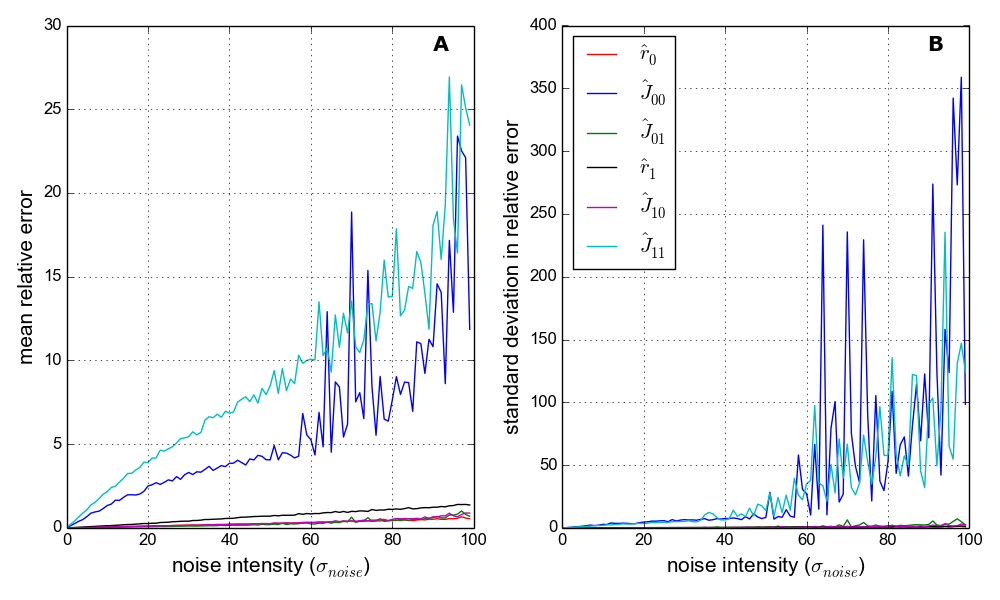
\includegraphics[width=0.67\textwidth]{{{figures/ensemble_params_vs_noise_nsamples_1000.ALL}}}
%\caption{Nonsense. 1000 samples used.} 
%\label{fig:ep_v_n}
%\end{figure}
%
%\begin{figure}[h]
%\centering 
%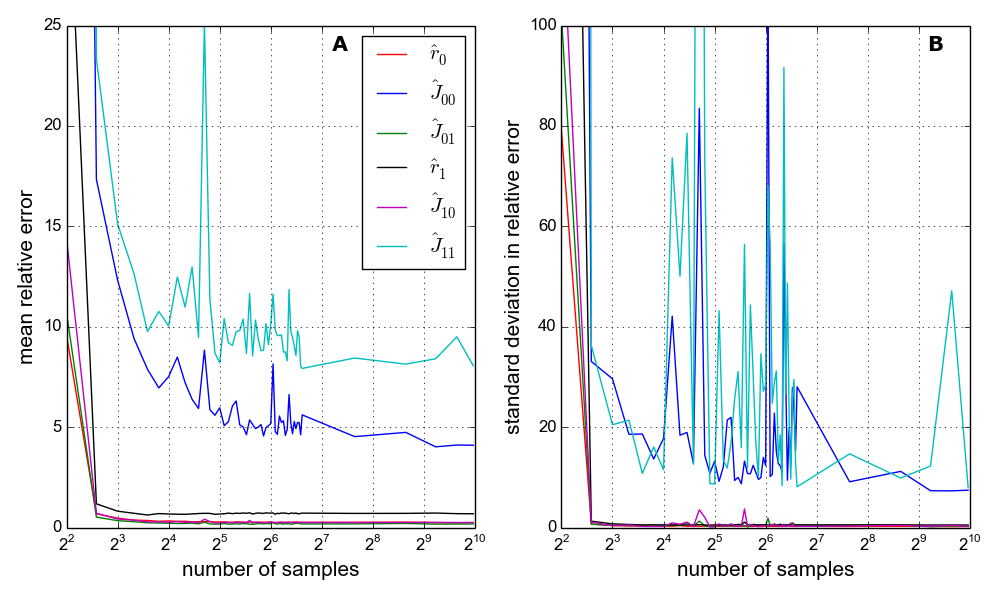
\includegraphics[width=0.67\textwidth]{{{figures/ensemble_params_vs_nsamples_noise_50.000000.ALL}}}
%\caption{Nonsense. Noise is 50.} 
%\label{fig:ep_v_ns}
%\end{figure}

\section{Results: IBM as data generator}
\label{sec:ibm}

%NEED TO WRITE ABOUT CONSTRAINTS ON TOPOLOGY. AND DISCUSS FOCUS ON ANTAGONISTIC INTERACTIONS ONLY, AND NO HL. ALSO STATE THAT ALL SIMUALTIONS HAVE TRANSIECNE REMOVED (HOW MANY TIME STEPS?)

In this section we apply the inference method to population dynamics simulated using the IBM model. Here the dynamics is not explicitly governed by differential equations, and so this represents a more realistic test of the method. The analysis is extended to systems with three and five species, which significantly increases the complexity of the problem. In particular these systems have missing links, i.e. potential interactions between species which do not actually occur. We investigate if the inference method can detect these missing links. All simulations run using the IBM have the initial 2000 time steps removed unless otherwise stated. Similar to previous chapters this removal ensures that the initial period of transience, as the system relaxes from the initial conditions, is not included in our analysis. Before presenting the results of the inference method we introduce an extension that allows the fitting of the GLV with topological constraints (section \ref{sec:top_const}). We also analysis certain properties of the IBM output, in order to justify the fitting of the GLV model to its dynamics (section \ref{sec:prop_ibm_gen}). 

%We first characterise the functional forms of the intrinsic growth and mortality rates for prey and predator species. We then determine that the functional responses in the IBM are approximately linear. And argue that this would be expected because there is no saturation or prey handling included in the model. We then present results for:
%\begin{itemize}
%	\item Two species: works well. Identifies with is prey, which is predator. IS closely resembles GLV estimates. Rate parameters and biomass flows accurately recovered.
%	\item Three species: Good rate estimates and biomass flows. The inference method often finds that the best fit is given by a model where the top predator is eaten by the plant species! Explore ways to identify correct model topology. Inconclusive. Model fit is good for intermediate species.
%	\item Five species: Similar results to three species. In particular, we cannot reliably identify the correct topology, and the best fit model is often one in which the top-predator is eaten by one of the plants.
%	\item 60 species communities, with species group into trophic levels such that the network size is reduced to four.   Will present a brief discussion of this. But based on the results for three and five species it is not worth going into too much detail. There is clearly a problem... 
%\end{itemize} 
%Discuss postulate of parenthood.

%In this section we apply the methodology for inferring species interactions to the IBM simulations. In the previous section we have seen that the method works well when fitting the GLV to two species predator-prey dynamics simulated with ODE models. In the case that the dynamics is governed by the Lotkva-Volterra equations, and in the absence of noise, fitting the GLV model produces true estimates of the underlying parameters which include the inter-specific interaction strengths. The estimates require relatively few samples in order to achieve high accuracy, and which converge on the true parameter values as the sampling intensity increases. However as noise is added to the simulations the accuracy of the estimates decreases. In particular we found that, in the presence of noise, the estimates do not converge on the true parameter values - that is, noise introduces systematic error in to the estimates. In the case that the dynamics are governed by the Holling II model matters are complicated - but in general we find that the GLV can approximately capture the strength of species interactions (and also the dynamics?), provided there is not too much noise, and the FR is not too non-linear\footnote{This is all need to be demonstrated - WORK TO DO!}.
%
%Can the IBM dynamics by approximated by the GLV model? The hypothesis is that is can. Argue this..and refer to previous mention of LV type dynamics. Refer forward to testing linearity of FR. Exponential growth and decay, linear FR. However there are certain problem/factors that may hinder this approach/represent a departure from GLV dynamics...Noise, spatial effects, bioenergetic model - time delay? Immigration (one component of noise).
%The issue of noise is important since, as we have shown in chapter REF, there is a strong stochastic component to the IBM simulations. 
%Modelling individuals, not biomass or energy. Is this problematic? Set herb-frac to 1. Other issues?

\subsection{Topological constraints on the GLV}
\label{sec:top_const}

Fitting the full GLV model to population dynamics never produces estimates of interaction strength that are exactly equal to zero. Therefore in some cases it is desirable to constrain the interaction topology which is used to fit the dynamics, in order to compare how the GLV fit performs without certain links. The method for conducting this constrained fit is outlined here. We reproduce the analytic solution for the GLV fit to species $i$ (equation \ref{eq:timme_a2}):
\begin{equation}
\hat{J}_i = YG^T_i\left(G_iG^T_i\right)^{-1},
\end{equation}
where the matrices are defined as
\begin{equation}\label{eq:timme888}
Y_{i} = 
\begin{pmatrix}
  \hat{\dot{y}}_{i1} & \hat{\dot{y}}_{i2} & \cdots & \hat{\dot{y}}_{iM}
\end{pmatrix}\\
\in{\mathbb{R}^{1 \times M}},
\end{equation}

\begin{equation}\label{eq:timme99}
\hat{J}_{i} = 
\begin{pmatrix}
  r_i & J_{i1} & J_{i2} & \cdots & J_{iN}
\end{pmatrix}\\
\in{\mathbb{R}^{1 \times(N+1)}},
\end{equation}

\begin{equation}\label{eq:timme10}
G_{i} = 
\begin{pmatrix}
  f_{i1}  &    f_{i2} & \cdots & f_{iM}         \\
  g_{i11} & g_{i12} & \cdots & g_{i1M} \\
  g_{i21} & g_{i22} & \cdots & g_{i2M} \\
  \vdots    & \vdots    & \ddots & \vdots    \\
  g_{iN1} & g_{iN2} & \cdots & g_{iNM} \\
\end{pmatrix}\\
\in{\mathbb{R}^{(N+1)\times M}}.
\end{equation}
%
We can constrain the species $j$ with which species $i$ is allowed to interact in the fitted model. By removing the element $\hat{\dot{y}}_{ij}$ from $Y_{i}$, and the $j^{th}$ row from $G_i$, we effectively remove the $j^{th}$ species from the error minimisation. In this case we obtain an estimate $\hat{J}_{i} \in \mathbb{R}^{1 \times(N)}$ (rather than $\mathbb{R}^{1 \times(N+1)}$). As many species as required can be removed from the error minimisation, and when the full estimated interaction matrix $\hat{J}$ is reconstructed we insert zeros into the corresponding matrix entries.
%\subsection{Testing functional response (and intrinsic growth functions)}

\subsection{Properties of the data generator}
\label{sec:prop_ibm_gen}

Before applying the inference method to \emph{data streams} derived from IBM simulations, we consider certain properties of the IBM. This model has yet to be used to simulate communities with a small number of species. In previous chapters we have studied simulated communities of no less than 30 species. The simulation of smaller communities requires some parameter adjustment in order to obtain dynamics that are amenable to our goal of estimating the strength of species interactions. We also consider the functional forms generated by the model, in order to determine the appropriateness of fitting a GLV model to the dynamics. Specifically we study the intrinsic growth functions of basal and non-basal species, and the functional response of non-basal predators. 

Unlike the ODE models used as the \emph{data generators} in section \ref{sec:results}, the IBM does not allow us to calculate analytic forms for the interaction strengths (using the metric $\alpha$, defined in section \ref{sec:interaction_strength}). Rather the interaction strengths in the IBM emerge from the local interactions between individuals during the simulation. In this sense the use of the IBM as \emph{data generator} represents a step towards \emph{realism} in testing the inference method. However, the unavailability of analytic forms for the interaction strengths raises the question of how to evaluate the performance of the inference method. The simplest check, and the most fundamental concern, is to determine if the fitted GLV parameters correctly identify which species are prey, which species are predators, and which species interact. That is, does the method identify 	the correct interaction network topology. Further to this we are interested in determining how accurate the GLV estimates of interaction strength are, compared to some other measure of interaction strength derived from the IBM output. One possibility is to use the metric IS (equation \eqref{eq:is3}), which has been used hitherto in the thesis. However this metric only quantifies the per-capita effect on the prey population, per-capita of the predator. Therefore IS is analogous to the GLV estimate $\hat{J}_{01}$. In section \ref{sec:ibm_2sp_res} we develop an alternative metric that allows us to quantify the accuracy all the inferred GLV parameters (including inter-specific interaction strengths, and the intrinsic parameters for each species).   



\begin{figure}
	\centering
	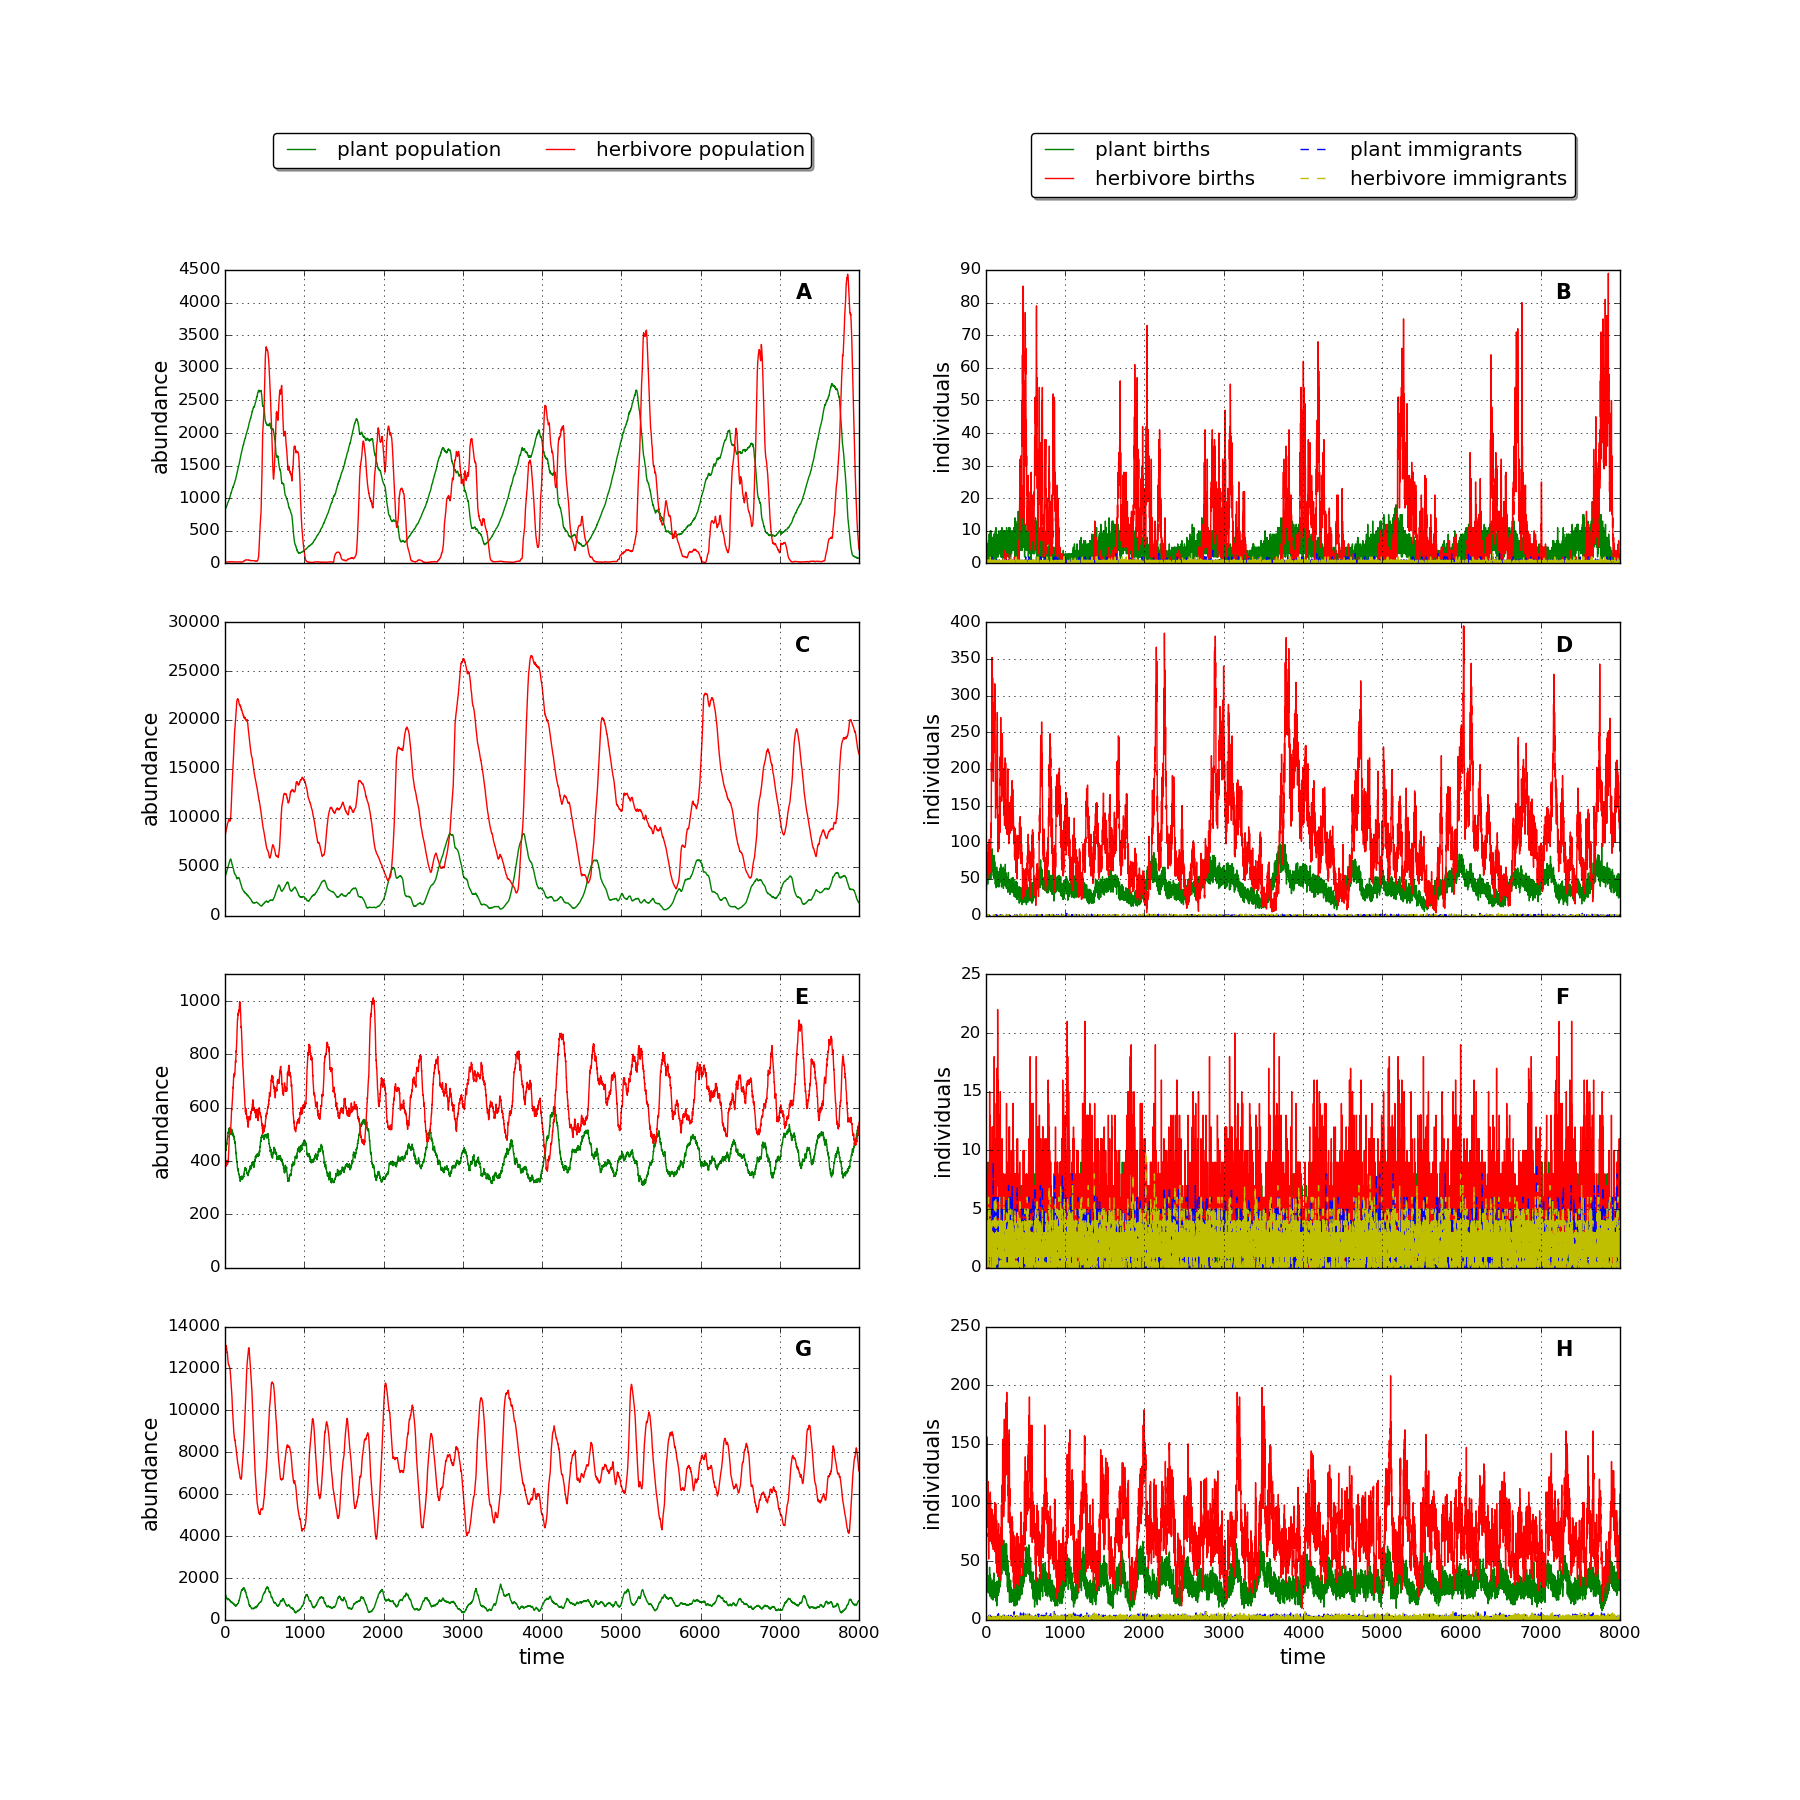
\includegraphics[width=\textwidth]{{{figures/IBM/2species/example_dynamics_2sp_ir_rr}}}
	\caption[Example dynamics of the IBM for two species]{\textbf{Example dynamics of the IBM for two species} with different reproduction rates (RR) and immigration rates (IR). Here low and high RR are 0.01 and 0.1 respectively. Low and high IR are $10^{-4}$ and $10^{-5}$ respectively. \textbf{Left column}: Population dynamics of the two species. \textbf{Right column}: Time series of births and immigrations for both species. \textbf{First row}: low RR and low IR. \textbf{Second row}: high RR and low IR. \textbf{Third row}: low RR and high IR. \textbf{Fourth row}: high RR and high IR.}
	\label{fig:2sp_dynamics}
\end{figure}

Figure \ref{fig:2sp_dynamics} shows the dynamics of the IBM model, simulated with two species, for various parameter values. One species is a plant, the other is a herbivore which feeds on the plant. Throughout this section IBM simulations use a value of $1.0$ for the parameter \emph{HERB\_FRACTION}, rather than the default value of $0.7$.  This parameter defines the fraction of the energy/resource of a plant individual that is taken when it is fed on by a consumer. The use of the value $1.0$ means that any feeding interaction results in the death of the plant individual, simplifying the interpretation of the modelling and the calculation of interaction strengths. Further to this parameter adjustment, we compare the effects of changing the immigration rate parameter (IR), and the reproduction rate parameter (RR), on two species dynamics.

The immigration parameter IR represents a source of noise in the dynamics. This fact, although intuitive, was revealed explicitly by \emph{recurrence quantification analysis} in chapter \ref{chap:stress_testing}. As we saw in section \ref{sec:results}, the performance of the inference method can be highly sensitive to noise, especially when the functional response of the predator is non-linear (see below). However the noise introduced by immigration is slightly different from the noise modelled in section \ref{sec:results}. In the ODE models multiplicative noise was used, such that the noise term vanished for zero populations and the \emph{postulate of parenthood} was not violated (section \ref{sec:noise}). In the IBM immigration represents a source of individuals that is not dependent on species populations in the landscape, and therefore net immigration does not fall to zero when no individuals are present. The IBM with non-zero IR violates the \emph{postulate of parenthood}. However we argue that the noise introduced by immigration is still likely to cause systematic error in the estimates of interaction strengths. Importantly there is another source of noise resulting from the fact that the dynamics of the IBM are inherently stochastic. Individuals move around, interact and reproduce at random. It is not clear at this stage which source of noise is more significant. In an attempt to reduce the error introduced by immigration we use IR values that are low compared to those used in chapter \ref{chap:varying_immigration_rate}. For \emph{zero IR} we determined that the two species IBM dynamics was unstable. The herbivore species invariability went extinct (results not shown), which is consistent with results from chapter \ref{chap:stress_testing}. Therefore two non-zero IRs were selected: $10^{-4}$ and $10^{-5}$. The former value is equal to the lowest IR studied in chapter \ref{chap:varying_immigration_rate}, but in the context of this chapter is referred to as the \emph{high IR}. The latter value is an order of magnitude smaller, and therefore is referred to as the \emph{low IR} in what follows. 

The top two rows of figure \ref{fig:2sp_dynamics} show dynamics simulated with the \emph{low IR}, and the bottom two rows with the \emph{high IR}. The left column shows the population dynamics, while the right column shows the number of immigrants and individuals born for both species on each time step. Panels A and E show dynamics that use the \emph{default reproduction rate} (RR$=0.01$). In the low IR case (panel A) we see that the populations display \emph{relaxation-type} oscillations, with the herbivore population falling close to zero for different periods of time with intermittent spiking. Such oscillations are sensitive to noise because a small stochastic increase in population during the relaxation phase can induce spiking. It was experimentally determined that the presence of such oscillations hampered attempts to infer species interaction strengths (results not shown). By increasing RR the decline in the plant population, which causes the crash in predator population, is softened (a similar argument was used in section \ref{sec:rr_v_p}). Panels C and G show dynamics with an increased RR of 0.1. In the low IR case (panel C), although there are still large amplitude oscillations, the herbivore population no longer relaxes close to zero. In all simulations that follow we use the value RR$=0.1$ in order to avoid relaxation-type oscillations.

Another consequence of increasing RR is that it increases the population levels of both species, on average. However, as we see from panels C and G, most of this benefit in conferred on the herbivore rather than the plant. Presumably the reason for this is strong predation by the herbivore, which regulates the plant populations. There is no predation pressure on the herbivore, only the effects of intrinsic mortality. The increased species abundances under high RR reduce dependence on immigration. In panels D and H the number if immigrants is barely visible, compared to the number of parented-births for both species. This observation suggests in this parameter regime that the contribution of noise resulting from immigration is low, compared to the inherent stochasticity of the IBM dynamics.

\begin{figure}
	\centering
	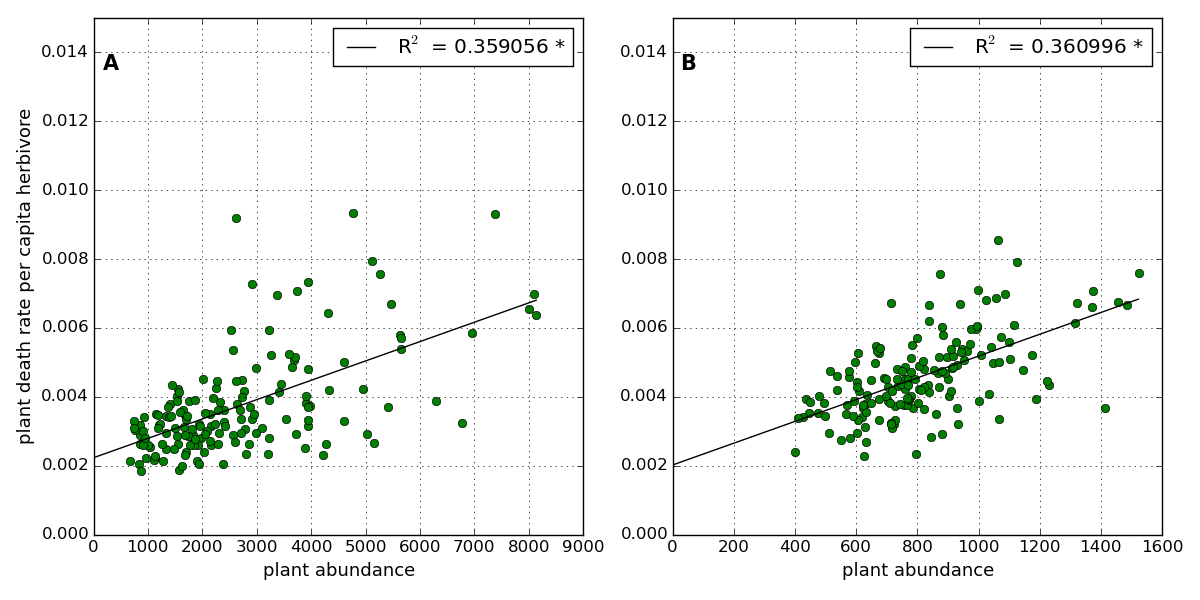
\includegraphics[width=\textwidth]{{{figures/IBM/2species/plant_FR}}}
	\caption[Functional response (FR) of the herbivore]{\textbf{Functional response (FR) of the herbivore} at two different immigration rates (IR), experimentally derived from two IBM simulations. Both simulations are of two species plant-herbivore systems, with reproduction rate (RR) 0.1 and run for 10,000 time steps. Each green circle represents the number of plants consumed during a window of 50 time steps, divided by the mean herbivore abundance during that window, plotted against the mean plant abundance during the window. The black lines represent linear regression fits to the data. $R^2$ values for the fits are given in legends, and significance at $95\%$ confidence is indicated by *. \textbf{Panel A}: Low immigration rate ($IR=10^{-5}$). \textbf{Panel B}: High immigration rate ($IR=10^{-4}$).}
	\label{fig:plantFR}
\end{figure}
\begin{figure}
	\centering
	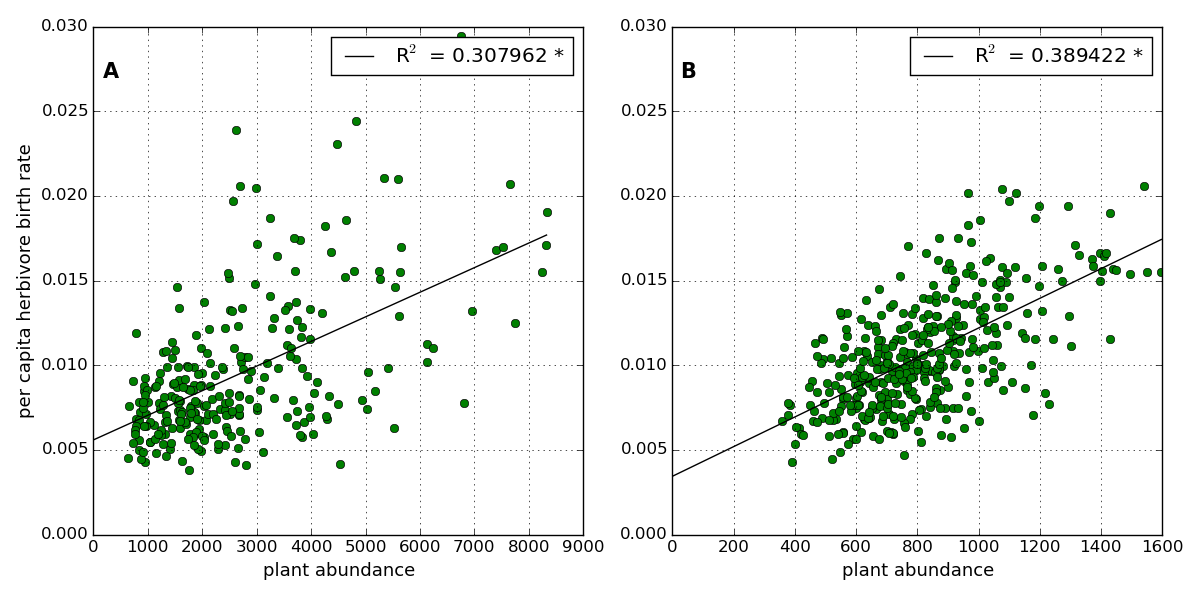
\includegraphics[width=\textwidth]{{{figures/IBM/2species/predator_FR}}}
	\caption[Numerical response (FR) of the herbivore]{Similar to figure \ref{fig:plantFR}, but for the \textbf{numerical response (NR) of the herbivore}. Each green circle represents the number of herbivores born during a window of 50 time steps, divided by the mean herbivore abundance during that window, plotted against the mean plant abundance during the window.}
	\label{fig:herbFR}
\end{figure} 

The dynamics in panels C and G in figure \ref{fig:2sp_dynamics} correspond to the parameter values (low and high IR respectively) which we will use in section \ref{sec:ibm_2sp} to study two species systems. In later sections, where we study larger systems, the same parameter values are also used. Figure \ref{fig:fr_example} shows the functional response (FR) of the herbivore at both low and high IR values. The FR is the same concept as introduced in the context of ODE modelling (section \ref{sec:models}). It defines the rate of prey consumption per-capita of predator. Here the FR is derived from the IBM simulation output by counting the number of plants consumed during a window of 50 time steps, and dividing that count by the mean herbivore abundance during the window. The plots in figure \ref{fig:fr_example} show the resulting FR values over the course of two simulations (panel A: low IR, panel B: high IR). From these plots we see that the FR appears to be approximately linear in plant abundance, with some deviation from linearity resulting from noise. Linear regression fits to the FRs indicate slightly less deviation from linearity at the high IR value (panel B). This observation is counter-intuitive based on results from previous chapters, where we have seen immigration act as a source of randomness in community dynamics.

Figure \ref{fig:herbFR} shows equivalent plots of the herbivore \emph{numerical response} (NR). NR is a similar concept to FR, but defines the per-capita birth rate of a predator as a function of its prey population \cite{solomon1949natural}. The NR is evaluated from the IBM simulation output in a manner analogous to that just explained for the evaluation of the FR. From the figure we observe that the NR is approximately linear. There is visibly more deviation from linearity in the low IR case (panel A), than in the high IR case (panel B). This observation is confirmed by the $R^2$ values of the linear regression fits. Therefore we conclude that noise resulting from stochasticity of the dynamics is more likely to be a source of error in the GLV fit, than is any non-linearity in the herbivore interaction functions. Indeed given that we do not model prey handling times in the IBM, it is reasonable that no signature of predator saturation is detected \cite{holling1959some}. Furthermore it appears that stochastic effects are greater at high IR ($10^{-4}$) than at low IR ($10^{-5}$).

\begin{figure}
	\centering
	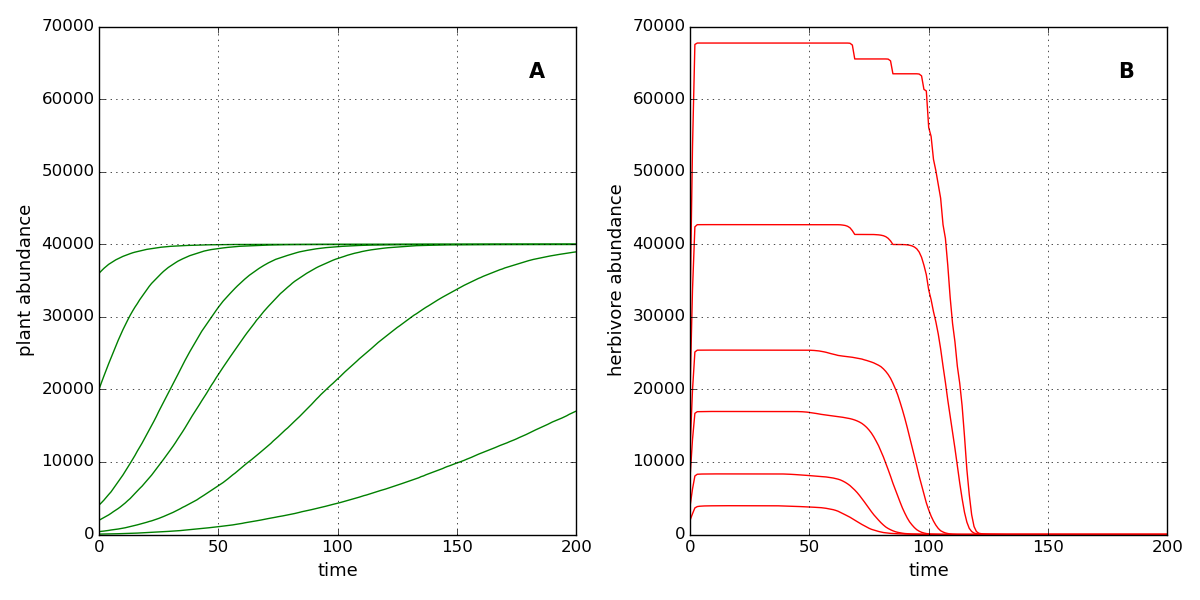
\includegraphics[width=\textwidth]{{{figures/IBM/2species/intrinsic_fn}}}
	\caption[Intrinsic growth and mortality functions]{\textbf{Intrinsic growth and mortality functions} derived experimentally from two species IBM simulations. \textbf{Panel A}: How the plant population grows from different initial abundances, in the absence of any herbivores. \textbf{Panel B}: How the herbivore population declines from different initial populations, in the absence of any plants.} 
	\label{fig:intrinsic}
\end{figure}

Figure \ref{fig:intrinsic} shows experimentally derived forms of the intrinsic growth and mortality functions of the plant (panel A) and herbivore (panel B). These results were obtained by simulating landscapes with different starting abundances of a single species, without any individuals of the other species. In all cases IR$=0.0$, such that the only new individuals are due to reproduction. The intrinsic growth of the plant (panel A) is the classic \emph{logistic-type} sigmoidal shape that we expect when modelling a basal species. At low population densities the growth is near exponential, but at high population densities the growth rate is curtailed as the species approaches carrying capacity. In the case of plants the carrying capacity is equal to the number of landscape cells (40,000), since plant individuals may only occupy the \emph{inhabitant space} in each cell (see section \ref{sec:the_model}). The herbivore mortality function (panel B) is approximately sigmoidal. The initial conditions of the IBM are such that each individual begins with a random amount of energy. Therefore hebivores initially reproduce and the population level increases. However, the population (for the experiments depicted) never reaches the herbivore carrying capacity, which is twice the number of landscape cells (80,000) because non-basal individuals may occupy both the \emph{inhabitant} and \emph{visitor} spaces in a cell. The plateau in herbivore population is below carrying capacity because there is a finite amount of energy in the system. The decline in the population from the plateau is sharp, but display evidence of density-dependence similar to that observed for plant growth. The discrete steps visible at high population levels are possibly due to herbivores, which started with the same amount of energy, running out of energy at the same time. This feature suggests the possible existence of a \emph{time delay} in the herbivore response to changes in the availability of food. (This time delay may be thought of as an \emph{extinction debt}.) However, the main features of the intrinsic functions depicted, together with the near-linear functional forms seen in figures \ref{fig:fr_example} and \ref{fig:herbFR}, suggest that an attempt to fit the GLV model to the IBM dynamics is valid. 

%
%
%Carrying capacity: is there evidence for density dependent birth/death? - use this fact in later analysis. Also discuss that the carrying capacity will vary with the number of species, not just a single species thing (non-pairwise interactions in competition for space - argghh!)
%
%THE FR AND GROWTH RATE PLOTS NEED TO FOLLOW THE 2 SPECIES DYNAMICS PLOT.
%CHANGE OF PARAMS; HERBIVORES CONSUME WHOLE PLANT.
%THE TERMS LOW AND HIGH IR TAKE A DIFFERENT MEANING HERE FROM PREVIOUS CHAPTERS.



%\subsection{2 Species IBM model}
%\label{sec:ibm_2sp}
%IMPORTANT: carrying capacity depends on other species...introduce a new term into the model and test it?
%
%Define the model and what the inferred parameters represent:
%
%\begin{itemize}
%	\item $J_{01}$: per-capita of rate consumption of the prey
%	\item $J_{10}$: per-capita of rate reproduction of predator, due to consumption of prey. Not as well defined. But only source of predator births? Numerical response! (get REF)
%	
%	\item $J_{00}$: intra-specific regulation of prey growth - see carrying capacity experiment.
%	
%	\item $J_{11}$: intra-specific regulation of predator mortality? Check this. Expect zero? Or expect high number of predator means more reproduction because easier to find partner, therefore reduce mortality? Or increase birth rate. Not clear. Again SEE EXPERIMENT. 
%	
%	\item $r_0$: prey intrinsic growth rate. Estimate from exp?
%	
%	\item $r_1$: predator intrinsic mortality rate. Estimate from exp?
%\end{itemize}
%
%So we know what values to expect, or at least the signs. We can evaluate the model fit by comparing the values of these estimates with birth/death rates from the simulations. Although not totally fair. We can also simulate GLV with the inferred parameters - does it match. Is the equilibrium the same? And check the error function of the fit. We show all this in the results section below.

%\subsection{Extend methodology (3, 4 and 5 species)}
%
%MULTI-SPECIES DENSITY DEPENDENCE?!
%
%This does not require much since we presented a general framework previously. 
%
%Show 3 species dynamics with the two different RR. Conclude which is better. 

\subsection{Two species results}
\label{sec:ibm_2sp_res}

In this section results are presented for application of the inference method to \emph{data streams} derived from two species IBM simulations. In all cases the simulations contain one plant and one predator species, and the parameters used are those described in the previous section. Therefore we compare the case of low IR ($10^{-4}$) with high IR ($10^{-5}$). We first demonstrate the convergence of the GLV parameter estimates under different sampling conditions, and then develop a method for quantifying the accuracy of the estimates. All simulations were run for 10,000 time steps, and the initial 2000 time steps were discarded to remove the initial transience (in accordance with previous chapters).

%Here we compare the results of two species. 
%
%For a single IR we look at convergence of all 6 parameters (over the ensemble) - correct signs, correct magnitudes?
%
%Maybe repeat for other IRs and HL.
%
%We then show rate estimates as time series and introduce quality metric for this\footnote{Still not sure about this}.
%
%Demonstrate the quality decreases with IR and HL (box plot?).
%And how estimated parameters respond to the two HL scenarios (refer to previous findings). Hopefully support!
%DIFFERENCE BETWEEN M0 AND M1 - WHERE DO WE INTRODUCE TOPOLOGY RESTRICTION.

\begin{figure}
	\centering
	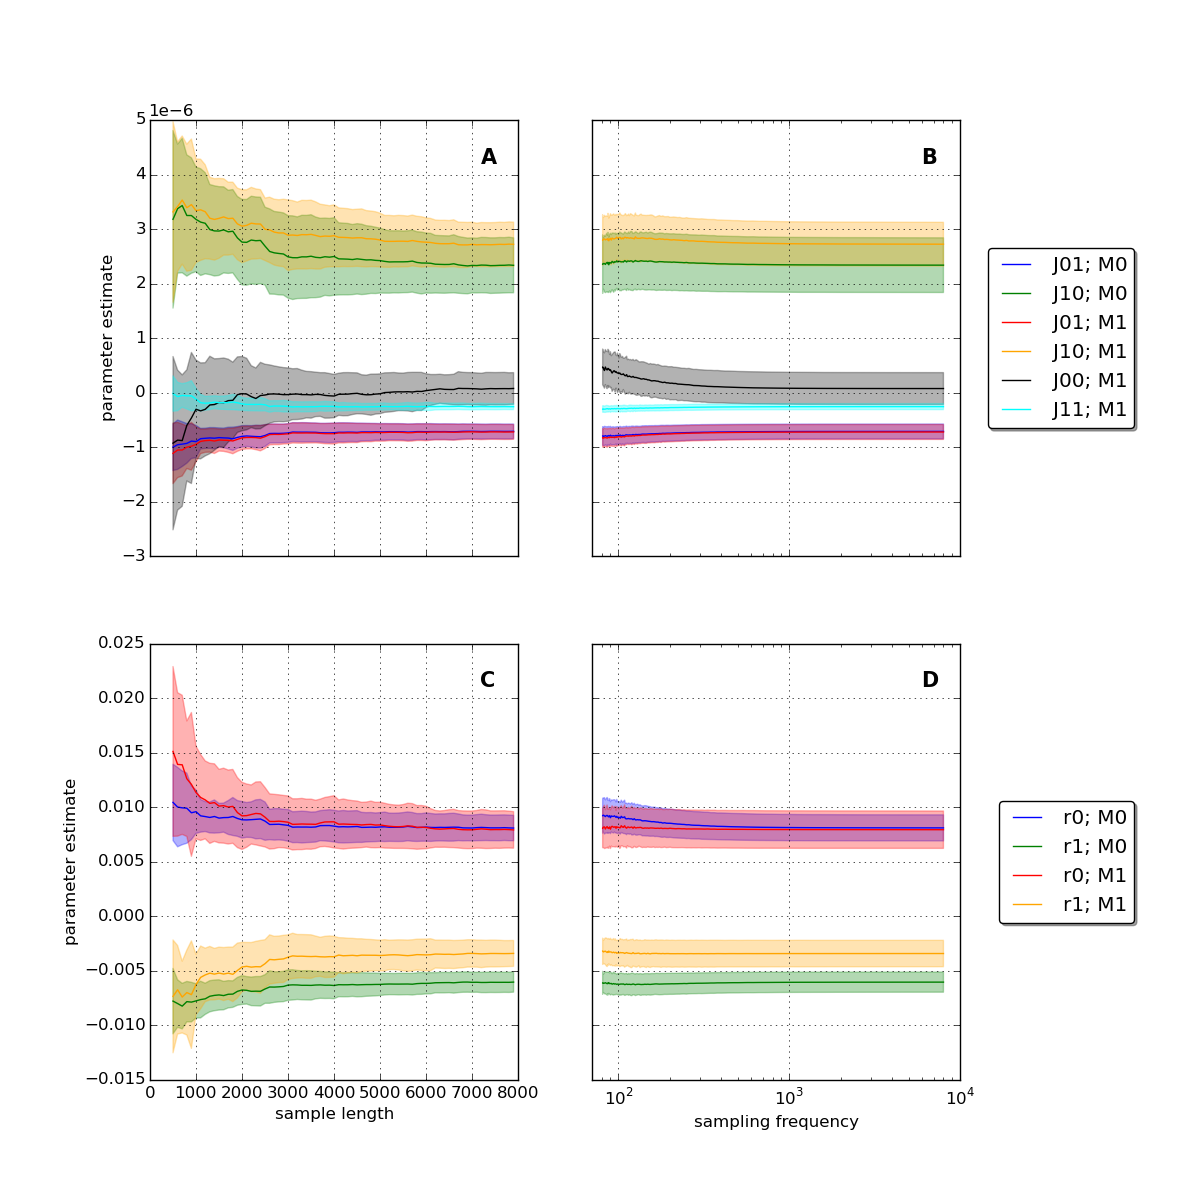
\includegraphics[width=\textwidth]{{{figures/IBM/2species/convergence_2sp_M0_M1_lowIR_rr0.1}}}
	\caption[Convergence of parameter estimates for low immigration rate, 2 species.]{\textbf{Convergence of parameter estimates for low immigration rate} ($IR=10^{-5}$). Solid lines represent mean values, shaded areas represent $\pm 1$ standard deviation, over 25 replicates. M0 indicates GLV model fit without intra-specific interactions ($J_{ii}=0$). M1 indicates GLV model fit without constraints on topology (see text). \textbf{Top row}: interaction strength estimates. \textbf{Bottom row}: growth rate estimates. \textbf{Left column}: convergence as sample length increased. \textbf{Right column}: convergence as sampling frequency increased.}
	\label{fig:2sp_convergence_LI}
\end{figure}

Figure \ref{fig:2sp_convergence_LI} shows how the GLV parameter estimates vary with sample length and sampling frequency in the case of \emph{low IR}. As in section \ref{sec:results} sample length is varied by taking samples of increasing length from the beginning of the population dynamics, using all consecutive time points. Sampling frequency is defined as the total number of samples  $F$, which are drawn at equal intervals from the full length of the dynamics. We compare the fits of two models, $M0$ and $M1$. M0 is the GLV model with the constraint that intra-specific interactions are equal to zero (see section \ref{sec:top_const}). M1 is the full GLV model without topological constraints. Each  model is fitted to 25 replicate simulations, so we can compare the mean and variability in estimated parameter values. In general we observe that the parameter estimates converge as the both sample length and sampling frequency are increased. This convergence is more rapid for increasing sampling frequency, suggesting that it is better to use samples drawn from the full length of the dynamics. That is, for a given number of samples, low resolution sampling of the full dynamics performs better than high resolution sampling of a subset. We also observe that the introduction of intra-specific interactions (M1) does not significantly affect estimates of prey interaction strength ($\hat{J}_{01}$), whereas it does affect estimates of predator interaction strength ($\hat{J}_{10}$). The estimates of $\hat{J}_{10}$ are also more variable than those of $\hat{J}_{01}$.

Figure \ref{fig:2sp_convergence_HI} shows the equivalent convergence plots for the \emph{high IR} case. Here the convergence of the estimates with sampling frequency is slower. From panels B and D we conclude that at least 1000 samples, distributed along the full length of the dynamics, are required to produce convergence of the estimates. As in the low IR case, we see that there is less variability in the estimates $\hat{J}_{01}$, than in $\hat{J}_{10}$, and that the latter estimates are more affected by the inclusion of intra-specific interactions. Note the scale on the y-axes of panels A and B are an order of magnitude larger than those in figure \ref{fig:2sp_convergence_LI}. The magnitudes of the estimates of inter-specific interaction strength ($\hat{J}_{01}$ and $\hat{J}_{10}$) are larger in the high IR case than in the low IR case. This observation is not consistent with results from chapter \ref{chap:varying_immigration_rate}, where it was seen that reducing the IR increased the mean value of IS for the community as a whole. However the observation is consistent with the argument that reducing IR reduces the probability of interaction between individuals, because there are fewer individuals present in the landscape. We suggest that the disparity between these results and those of the previous chapter is due to the limit behaviour of the IS metric (as previously argued), which biases the community level result as some populations approach zero. However it may also be the case that the GLV parameter estimates converge on values which are incorrect (i.e. do not faithfully represent the interaction strengths of the system). 

\begin{figure}
	\centering
	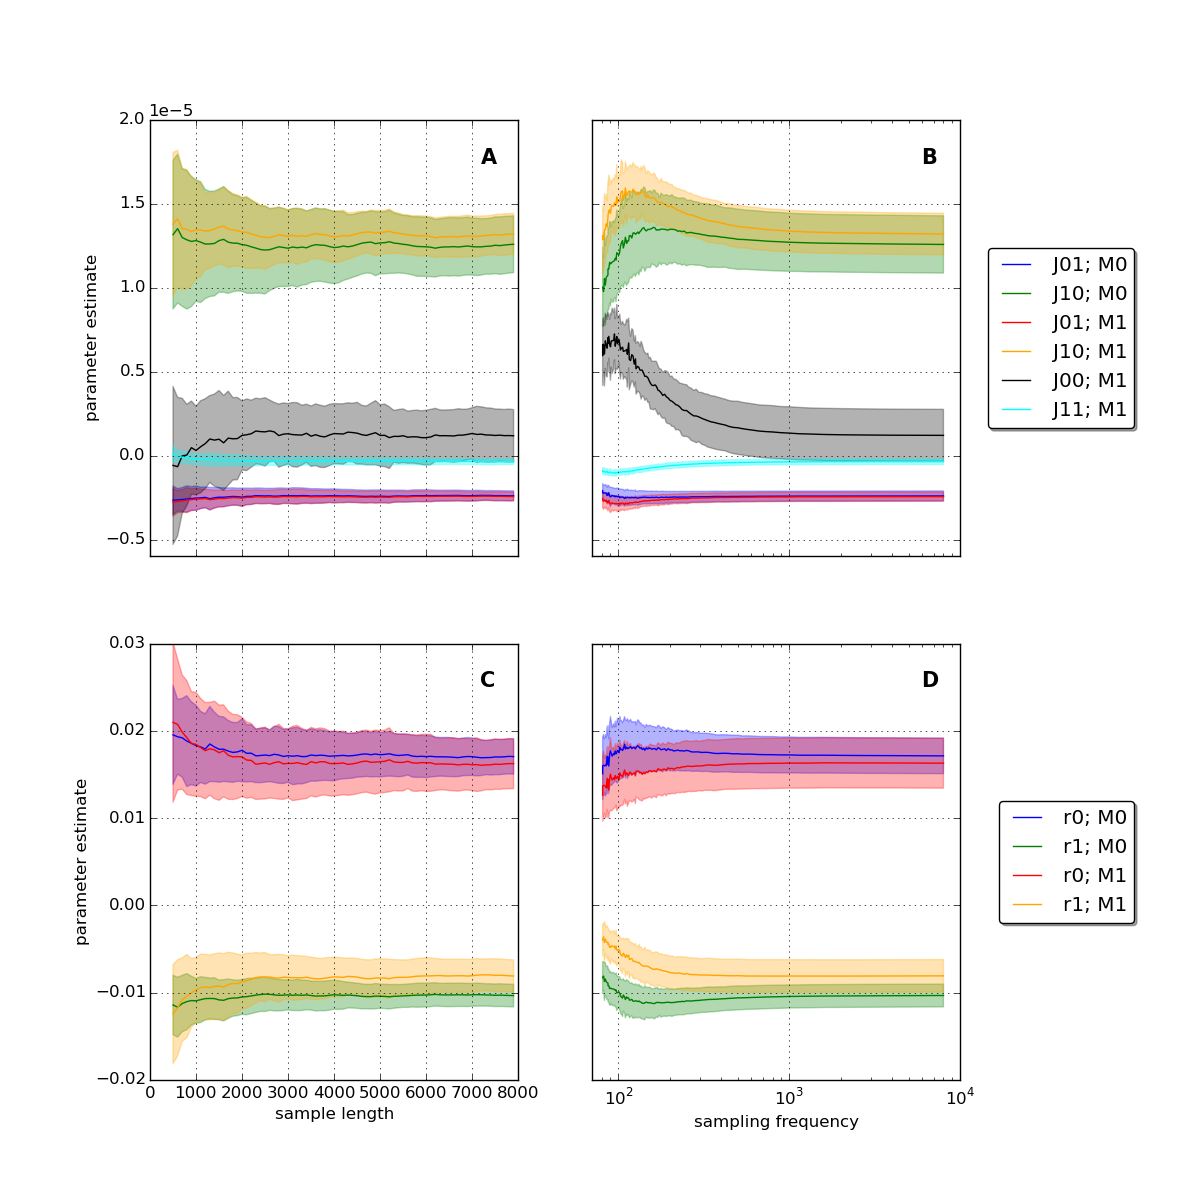
\includegraphics[width=\textwidth]{{{figures/IBM/2species/convergence_2sp_M0_M1_highIR_rr0.1}}}
	\caption[Convergence of parameter estimates for high immigration rate]{Similar to figure \ref{fig:2sp_convergence_LI}, but for \textbf{high immigration rate} ($IR=10^{-4}$).}
	\label{fig:2sp_convergence_HI}
\end{figure}

One possible way to determine the accuracy of the GLV parameter estimates is to simulate the GLV model using the fitted values, and compare the simulation to the original \emph{data stream}. In figure \ref{fig:inferred_dynamics_2sp} we use this method to compare the fits of $M0$ and $M1$ to a single \emph{low IR} simulation. Both fits use a \emph{sampling frequency} of 1000, based on the convergence results discussed above. In panel A we see that the simulated M0 fit produces oscillatory dynamics of comparable amplitude and period to those in the \emph{data stream}. In panel B we see that the introduction of intra-specific interactions dampens the oscillations in the fitted model (M1). However stochastic forcing may induce oscillations in a system with a stable equilibrium, such as this M1 fit. Therefore, under the correct noise conditions, the M1 fit may produce dynamics the are similar to the \emph{data stream}. Furthermore the shapes of the intrinsic functions, seen in section \ref{sec:prop_ibm_gen}, suggest the presence of intra-specific effects in the IBM. Therefore we conclude that simulating the fitted GLV is not an appropriate way to determine to accuracy of the fit.

\begin{figure}
	\centering
	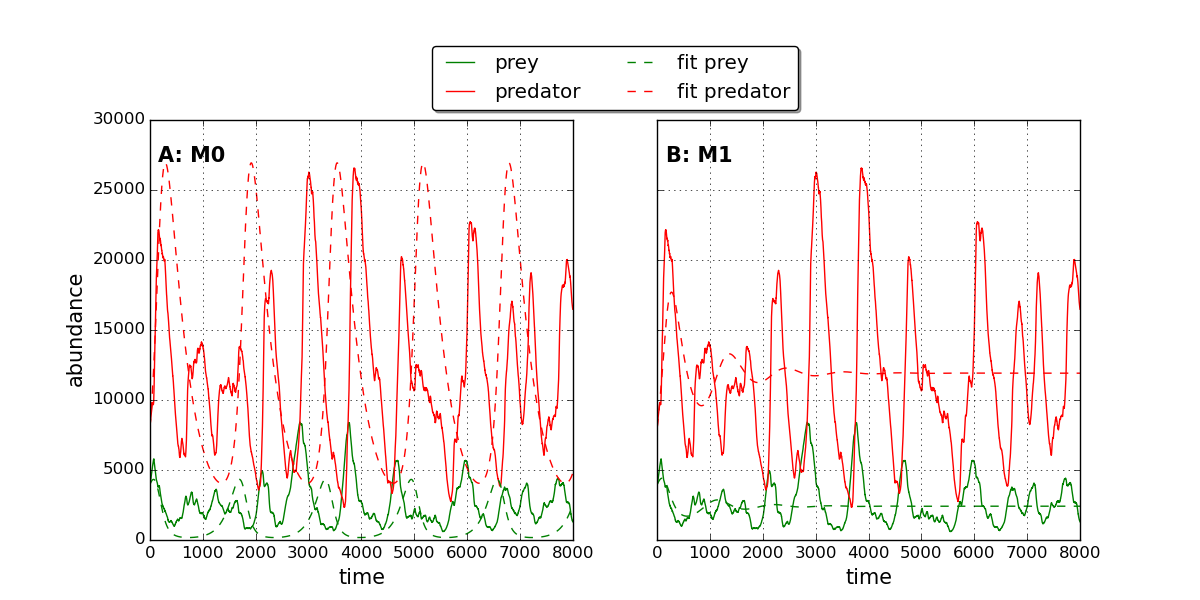
\includegraphics[width=\textwidth]{{{figures/IBM/2species/inferred_dynamics_2sp}}}
	\caption[Comparison between true and fitted dynamics]{\textbf{Comparison between true and fitted dynamics} for two different fitted models: M0 and M1. Solid lines represents the simulated IBM dynamics at \textbf{low IR} ($10^{-5}$). Dashed lines indicate a deterministic simulation of the fitted GLV, from the same initial conditions as the IBM time series. \textbf{Panel A}: M0 is GLV model with constraint that $J_{ii}=0$ (no intra-specific interactions). \textbf{Panel B}: M1 is full GLV with no constraints.}
	\label{fig:inferred_dynamics_2sp}
\end{figure}

Rather than simulating the fitted GLV model, we assess the predictions that the fitted model makes about the birth and death rates of both species. To compute these predictions the relevant parameters of the GLV are multiplied by some combination of the species population vectors. For example the prediction for \emph{predator births} is given by $\hat{J}_{10}X_0X_1$, where $X_0$ and $X_1$ are the true populations of the two species from the IBM simulation. The full set of definitions for the predicted rates of the fitted models are given in table \ref{tab:rate_est_2sp}. The GLV model fit without intra-specific interactions is named M0, as before. The GLV fit with intra-specific interactions raises the question of whether intra-specific interactions contribute to the birth or death rate of a species. Therefore the models labelled M1 and M2 refer to the same GLV fit, but M1 has the intra-specific terms added to the birth rate predictions, where M2 has them added to the death rate predictions. All rate predictions are plotted in figure \ref{fig:rate_estimates_2sp_li} for a low IR simulation, and in figure \ref{fig:rate_estimates_2sp_hi} for a high IR simulation. The model fits in all cases us a sampling frequency of 1000. The true birth and death rates for both species are plotted in green, for visual comparison with the predictions.

\begin{table}[h]
\centering
\begin{tabular}{
>{\columncolor[HTML]{EFEFEF}}l| l|l|l}
\hline
 \rule{0pt}{4ex}model & \cellcolor[HTML]{EFEFEF} M0 & \cellcolor[HTML]{EFEFEF} M1 & \cellcolor[HTML]{EFEFEF} M2 \\[10pt] \hline
\rule{0pt}{4ex}prey births &     $\hat{r}_0X_0$ & $\hat{r}_0X_0 + \hat{J}_{00}X_0^2$  & $\hat{r}_0X_0$ \\[10pt] \hline
\rule{0pt}{4ex}predator births &  $\hat{J}_{10}X_0X_1$ & $\hat{J}_{10}X_0X_1 + \hat{J}_{11}X_1^2$   & $\hat{J}_{10}X_0X_1$               \\[10pt] \hline
\rule{0pt}{4ex}prey deaths &   $\hat{J}_{01}X_0X_1$  & $\hat{J}_{01}X_0X_1$  & $\hat{J}_{01}X_0X_1 + \hat{J}_{00}X_0^2$   \\[10pt] \hline
\rule{0pt}{4ex}predator deaths & $\hat{r}_1X_1$   & $\hat{r}_1X_1$  & $\hat{r}_1X_1 + \hat{J}_{11}X_1^2$ \\[10pt] \hline
\end{tabular}
\caption[Demographic rate predictions.]{The way in which the various demographic rate predictions are calculated from the fitted model parameters, based on the observed populations. The vectors $X_0$ and $X_1$ are the full abundance time series of the plant and herbivore species respectively. Multiplication of these vectors is \emph{element-wise}.}
\label{tab:rate_est_2sp}
\end{table}

\begin{figure}
	\centering
	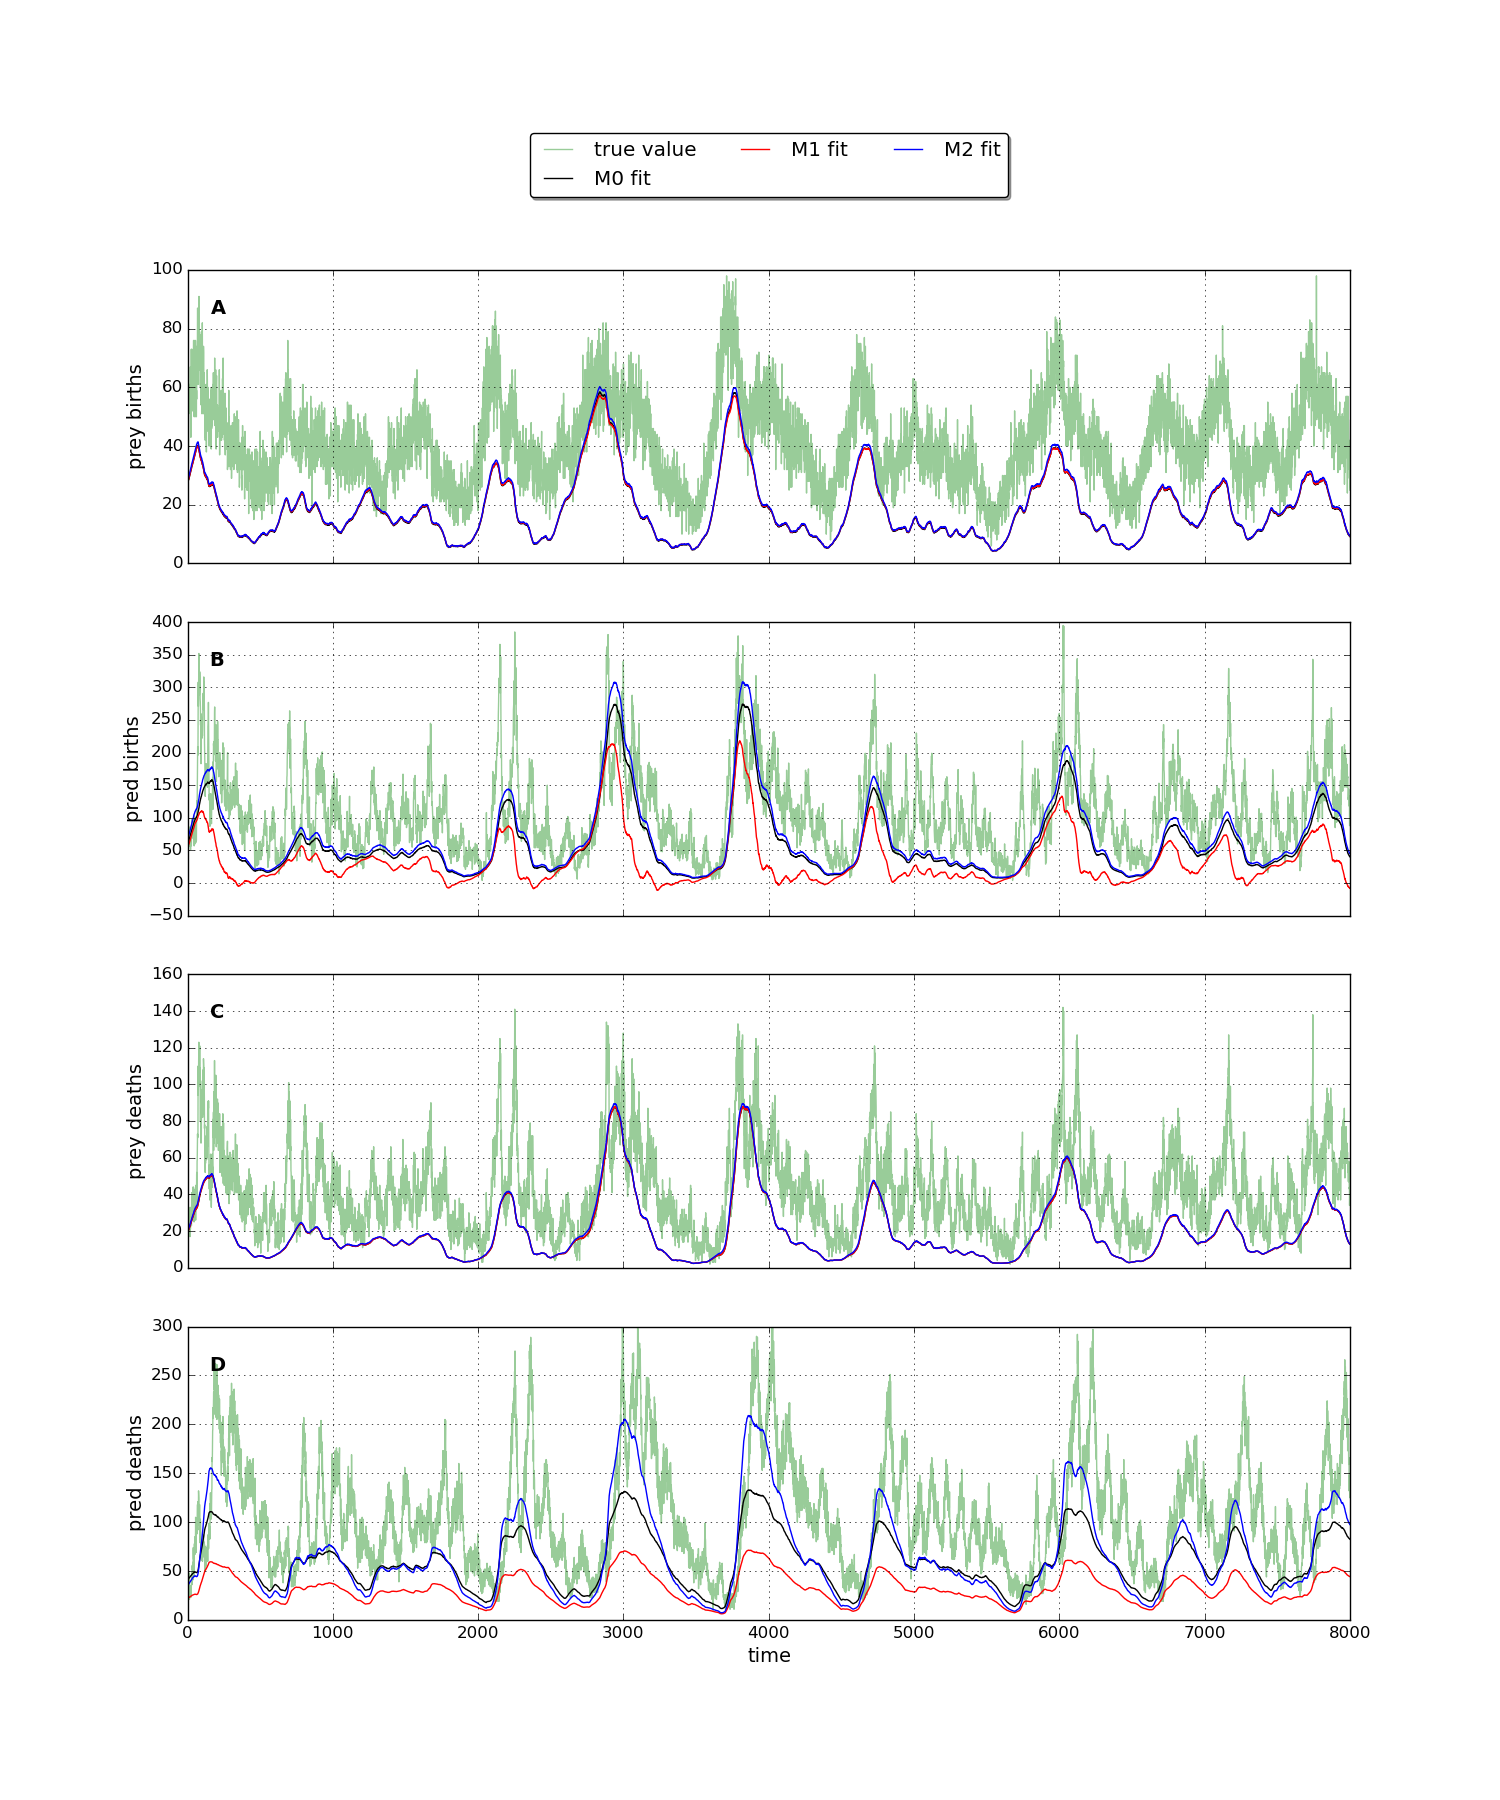
\includegraphics[width=\textwidth]{{{figures/IBM/2species/rate_estimate_series_2sp_hr_li}}}
	\caption[Two species demographic rate predictions, low IR.]{\textbf{Births and deaths predicted} by three different model fits: M0, M1, M2 (see text for model definitions). Green line is the true number of births and deaths for each species on each time step, recorded from the IBM simulation. Coloured lines represent model predictions of the number of births and deaths, based on the true population level of both species at each time step (see text for further details). The simulation was run using \textbf{low IR} ($10^{-5}$).}
	\label{fig:rate_estimates_2sp_li}
\end{figure}

\begin{figure}
	\centering
	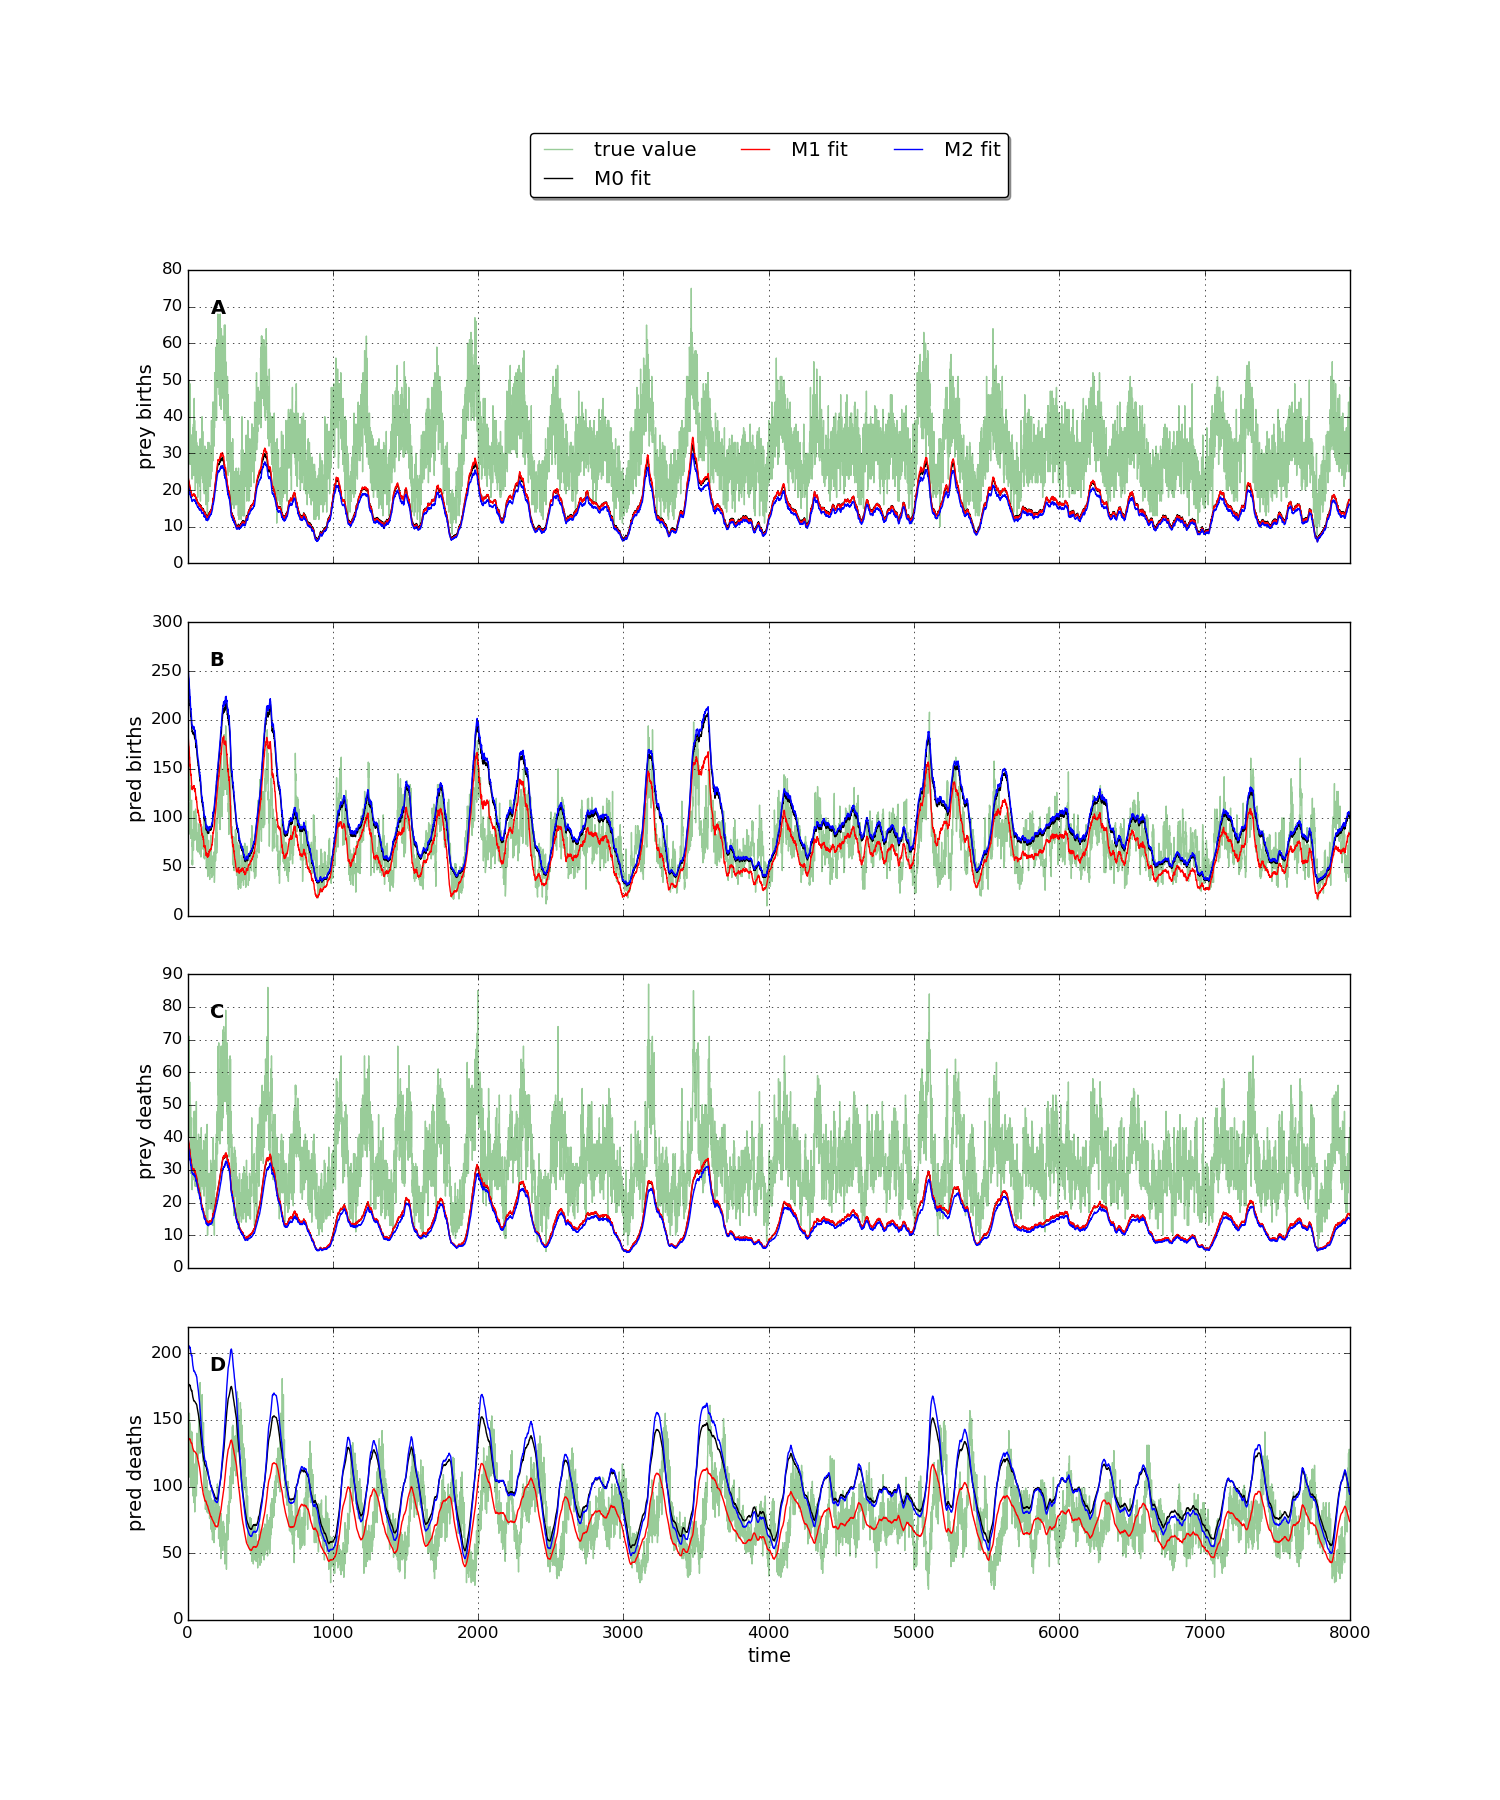
\includegraphics[width=\textwidth]{{{figures/IBM/2species/rate_estimate_series_2sp_hr_hi}}}
	\caption[Two species demographic rate predictions, high IR.]{Similar to figure \ref{fig:rate_estimates_2sp_li}, but for an IBM simulation at \textbf{high IR} ($10^{-4}$).}
	\label{fig:rate_estimates_2sp_hi}
\end{figure}

From figures \ref{fig:rate_estimates_2sp_li} and \ref{fig:rate_estimates_2sp_hi} we make the following observations. The periods of oscillation in the predicted rates match those of the true values closely. This is no surprise given that the predictions are calculated using the true population time series. However, in most case the predictions are also of comparable magnitude to the true values. Therefore the GLV fit can produce reasonable predictions of all demographic rates at any time point, given the abundance of both species. In the predictions of prey births and deaths there is little different between models M0, M1 and M2 (panels A and C, both figures). In the predictions of predator births and deaths, M1 clearly gives inferior results at low IR (panels B and D, figure \ref{fig:rate_estimates_2sp_li}). At high IR a difference is visible between the estimates of the three models (panels B and D, figure \ref{fig:rate_estimates_2sp_hi}) but it is hard to tell which model produces the best predictions. In order to quantify the performance of the different models in predicting species births and deaths we define a \emph{relative error metric}

\begin{equation}
<RE> \quad = \quad \frac{1}{T} \mathlarger{\mathlarger{\Sigma}}_{t=1}^T \left( \frac{|b(t) - p(t)|}{|b(t)|} \right),
\label{eq:rel_er_rate_2sp}
\end{equation}
%
where $T$ is the number of time steps in the dynamics, $b(t)$ is the true number of births or deaths on time step $t$, and $p(t)$ is the number of births or deaths predicted by the fitted model. This metric quantifies the mean relative deviation of the predictions from the true values over the full time series. 

\begin{figure}
	\centering
	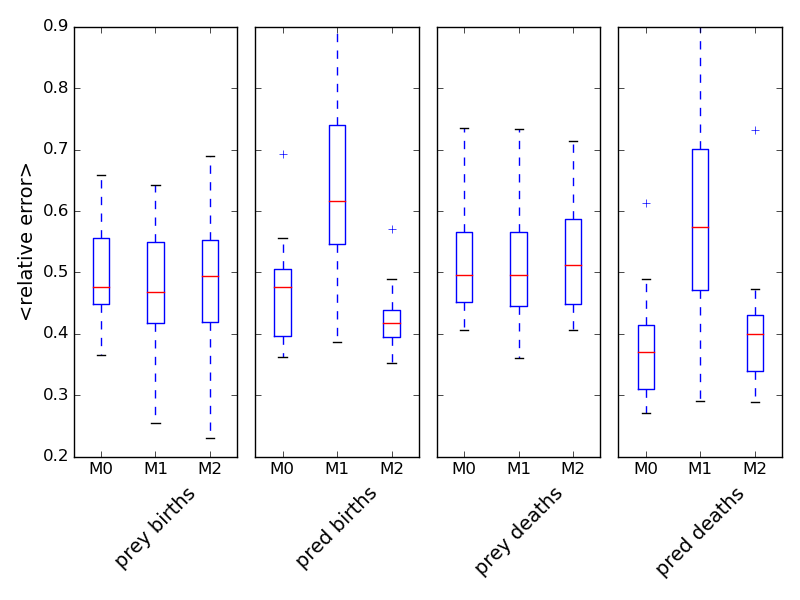
\includegraphics[width=\textwidth]{{{figures/IBM/2species/estimate_quality_2sp_lowIR}}}
	\caption[Relative error in rate predictions, low IR.]{\textbf{Relative error in the rates estimates} displayed in figure \ref{fig:rate_estimates_2sp_li} (prey and predator births/deaths). The relative error metric is defined in equation \eqref{eq:rel_er_rate_2sp}. The relative error statistics illustrated are derived from model fits to 25 replicate IBM simulations at \textbf{low IR} ($10^{-5}$). Boxes extend to the first and third quartiles of the data, and the red line indicates the median. Whiskers extend to show the range of the data, up to a maximum of 1.5 times the inter-quartile distance beyond which points are shown as outliers.}
	\label{fig:quality_2sp_li}
\end{figure}
\begin{figure}
	\centering
	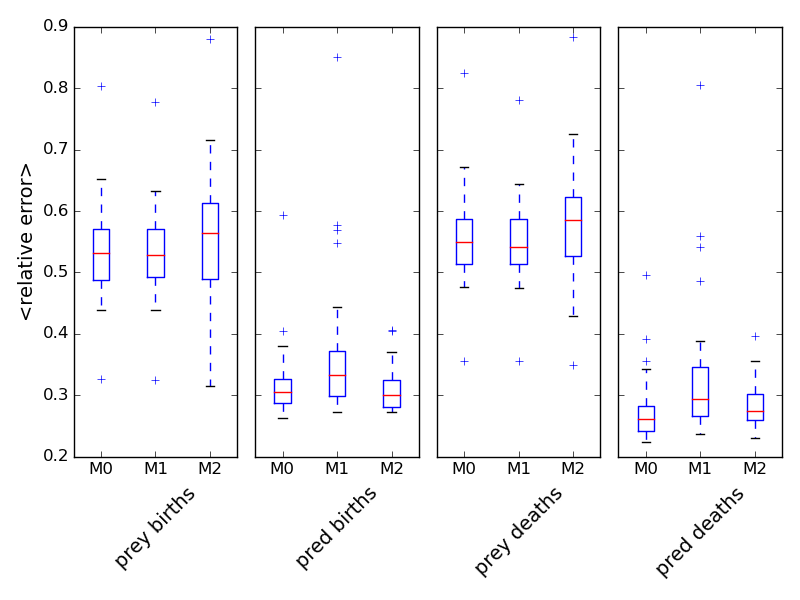
\includegraphics[width=\textwidth]{{{figures/IBM/2species/estimate_quality_2sp_highIR}}}
	\caption[Relative error in rate predictions, high IR.]{Similar to figure \ref{fig:quality_2sp_li}, but for results of model fits to 25 replicate IBM simulations at \textbf{high IR} ($10^{-4}$).}
	\label{fig:quality_2sp_hi}
\end{figure}
%

Figure \ref{fig:quality_2sp_li} summarises the relative error in the predicted births and deaths over an ensemble of 25 replicate simulations at low IR. The models are fitted to the simulated dynamics using a sampling frequency of 1000, as before. The fitted model parameters are then used to predict the births and deaths of both species, and the relative errors (RE) calculated as just described. For prey births and deaths there is little difference between the three models. Based on the median RE (red lines), the model M1 produces the best estimates by a narrow margin. For the predator estimates M1 clearly has higher errors, while M2 and M0 perform best for births and deaths respectively. Figure \ref{fig:quality_2sp_hi} shows the equivalent results for 25 simulations at high IR. The prey estimates have similar, or slightly higher, errors than in the low IR case, whereas the predator estimates show significantly lower errors. In the high IR case M2 performs the worst for the prey estimates, and M1 performs the worst for the predator estimates. Comparing across both low and high IR it appears that M1 is the correct model for the prey, while M2 is the correct model for the predator. However the inclusion of intra-specific interactions does not necessarily improve the rate predictions over those of M0. The use of M1 for prey predictions, and M2 for predator predictions, is consistent with the intrinsic functions derived in section \ref{sec:prop_ibm_gen}. That is, intra-specific interactions contribute to prey growth rates, but to predator mortality rates. 

\clearpage
\subsection{Three species results}
\label{sec:3sp_res_ibm}

In this section results are presented for fitting to 3 species IBM simulations of a \emph{food chain}. Each simulation contains a single plant species, a single herbivore species, and a single predator species which feeds only on the herbivore. This scenario represents the first test of the inference method in correctly identifying the interaction network topology. There is a potential link, between the plant and predator species, that is not present in the underlying interaction network. We investigate whether the method can detect the absence of this link. In all cases the GLV is fitted \emph{with} intra-specific interactions. According to the analysis in the previous section such interactions are taken to contribute to plant births, and to the deaths of the other two (non-basal) species, when rate predictions are made. We investigate the fitting of four candidate models (M0-3) with different constraints on interaction topology. These topologies are shown in figure \ref{fig:3sp_topo}, and are the only four possibilities that are connected (i.e. no isolated species). All models are subsets of M0, with M1 representing the true food chain that is simulated.

\begin{figure}
\centering
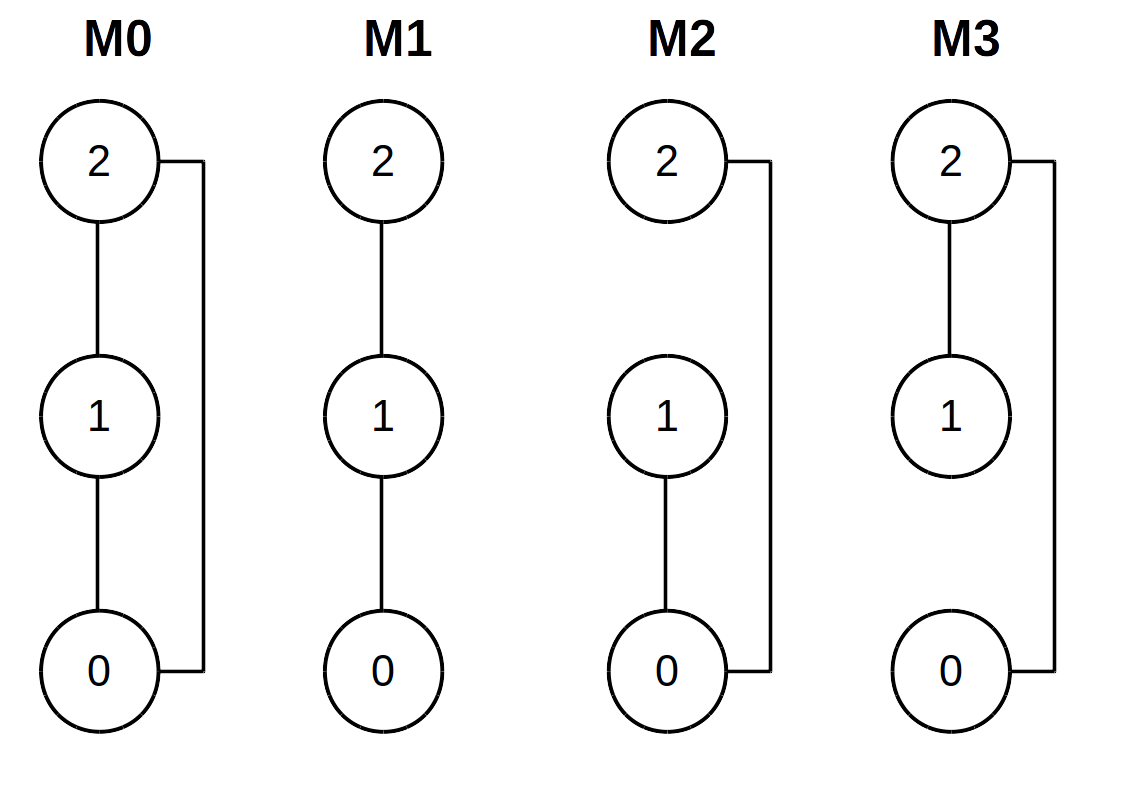
\includegraphics[width=0.5\textwidth]{{{figures/3sp_topologies}}}
\caption[Potential topologies for three species.]{The four candidate models investigated in this section. M0: fully connected. M1, M2, M3: one links removed. M1 is the `correct' model i.e. the food chain simulated by the IBM, to which the models are fitted. All four models include intra-specific interactions (self-loops), although these are not drawn.}
\label{fig:3sp_topo}
\end{figure}

\begin{figure}
	\centering
	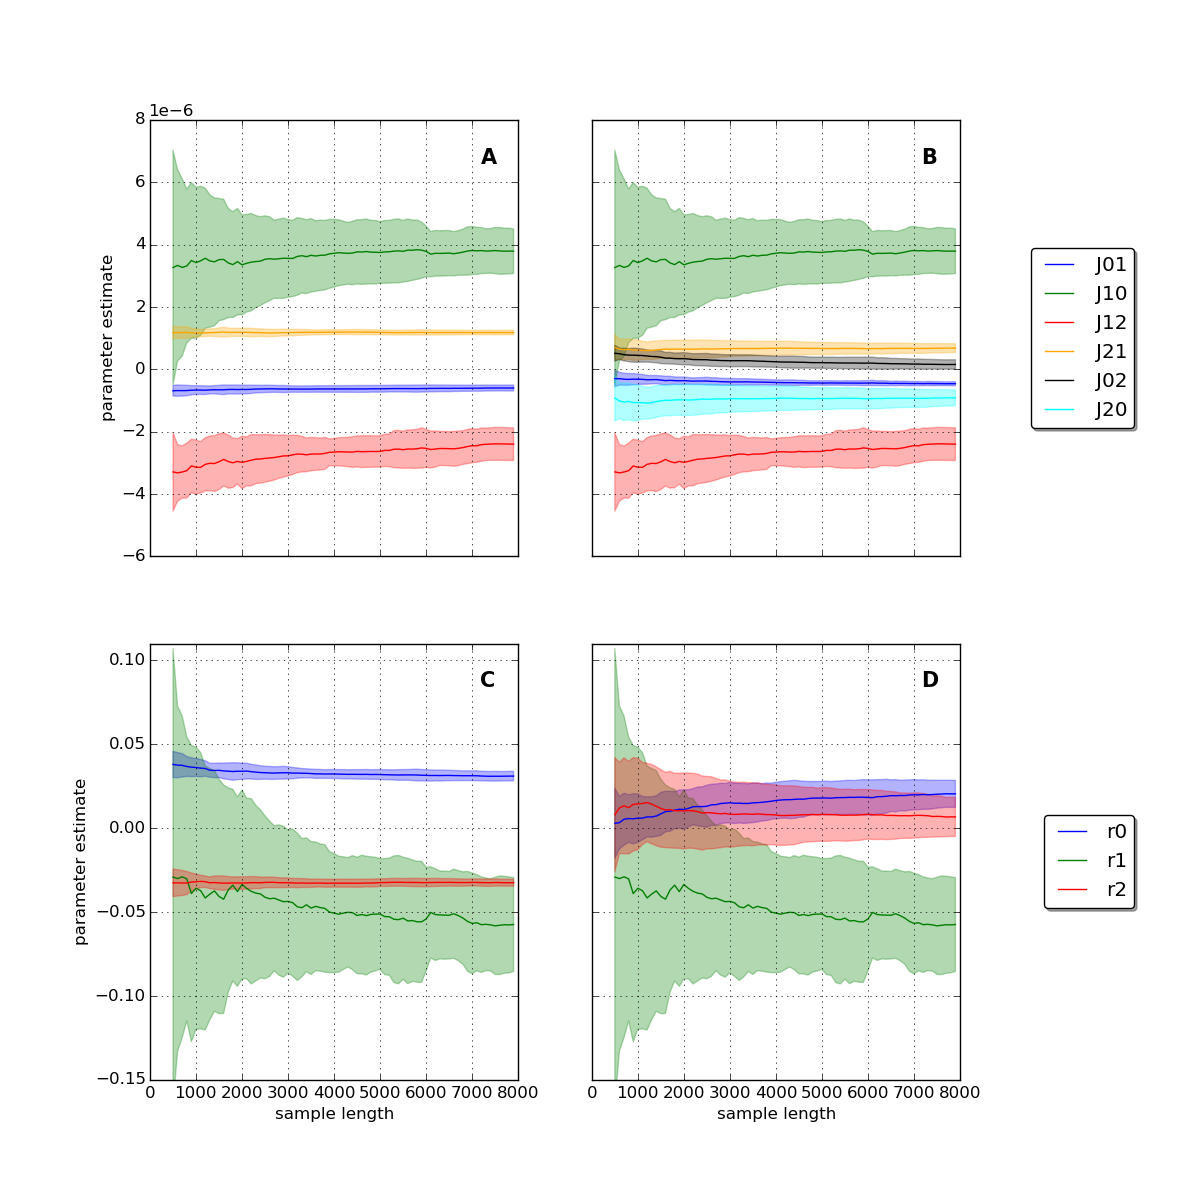
\includegraphics[width=\textwidth]{{{figures/IBM/3species/convergence_3sp_length_highIR}}}
	\caption[Convergence of parameter estimates, three species.]{\textbf{Convergence of parameter estimates with sample length for high immigration rate} ($IR=10^{-4}$). Two different models fitted to three species food chain dynamics. Inter-specific interactions (top row), and intrinsic parameters only (bottom row). Solid lines represent mean values, shaded areas represent $\pm 1$ standard deviation, over 25 replicates. Panels A and C show fits of model M1. Panels B and D show fits of the model M0. These models are illustrated in figure \ref{fig:3sp_topo}. Intra-specific interactions are included in the fits, but are not plotted for simplicity.}
	\label{fig:3sp_convergence_HI}
\end{figure}

Figure \ref{fig:3sp_convergence_HI} shows the convergence of parameter estimates with sample length for models M0 (right column) and M1 (left column), at high IR. The results at low IR are similar, and therefore not shown. The convergence depicted here is less convincing than in the two species case. In particular the estimates $\hat{J_{10}}$, $\hat{J}_{12}$ and all $r_i$, do not settle down as sample length is increased. A further concern is that, for all sample lengths, $\hat{J}_{02} > 0$ and $\hat{J}_{20} < 0$. These parameters correspond to the spurious link (not present in the true network), and the signs quoted are indicative of the \emph{plant species consuming the predator species}. It is worth noting that, when fitting M0, parameter that correspond to missing links will never be estimated as \emph{exactly} equal to zero. The hope is that either the model fit reveals that such parameters are of small magnitude, or that there is some other means by which to determine to correct topology.

%The two species results suggest that intra-specific interactions contribute to predator deaths, whereas they contribute to prey births\footnote{Actually it looks more like intra-specific interactions give negligible benefit!..Shit.}. This is problematic for rate estimation since we are starting from the position of not knowing which species are basal. For the purposes of calculating the rate we pretend that we know...This is in agreement with the Lotka-Volterra formulation.
%The alternative convention is that intra-specific interactions are 
%Extra term does not improve the estimates.

\begin{figure}
	\centering
	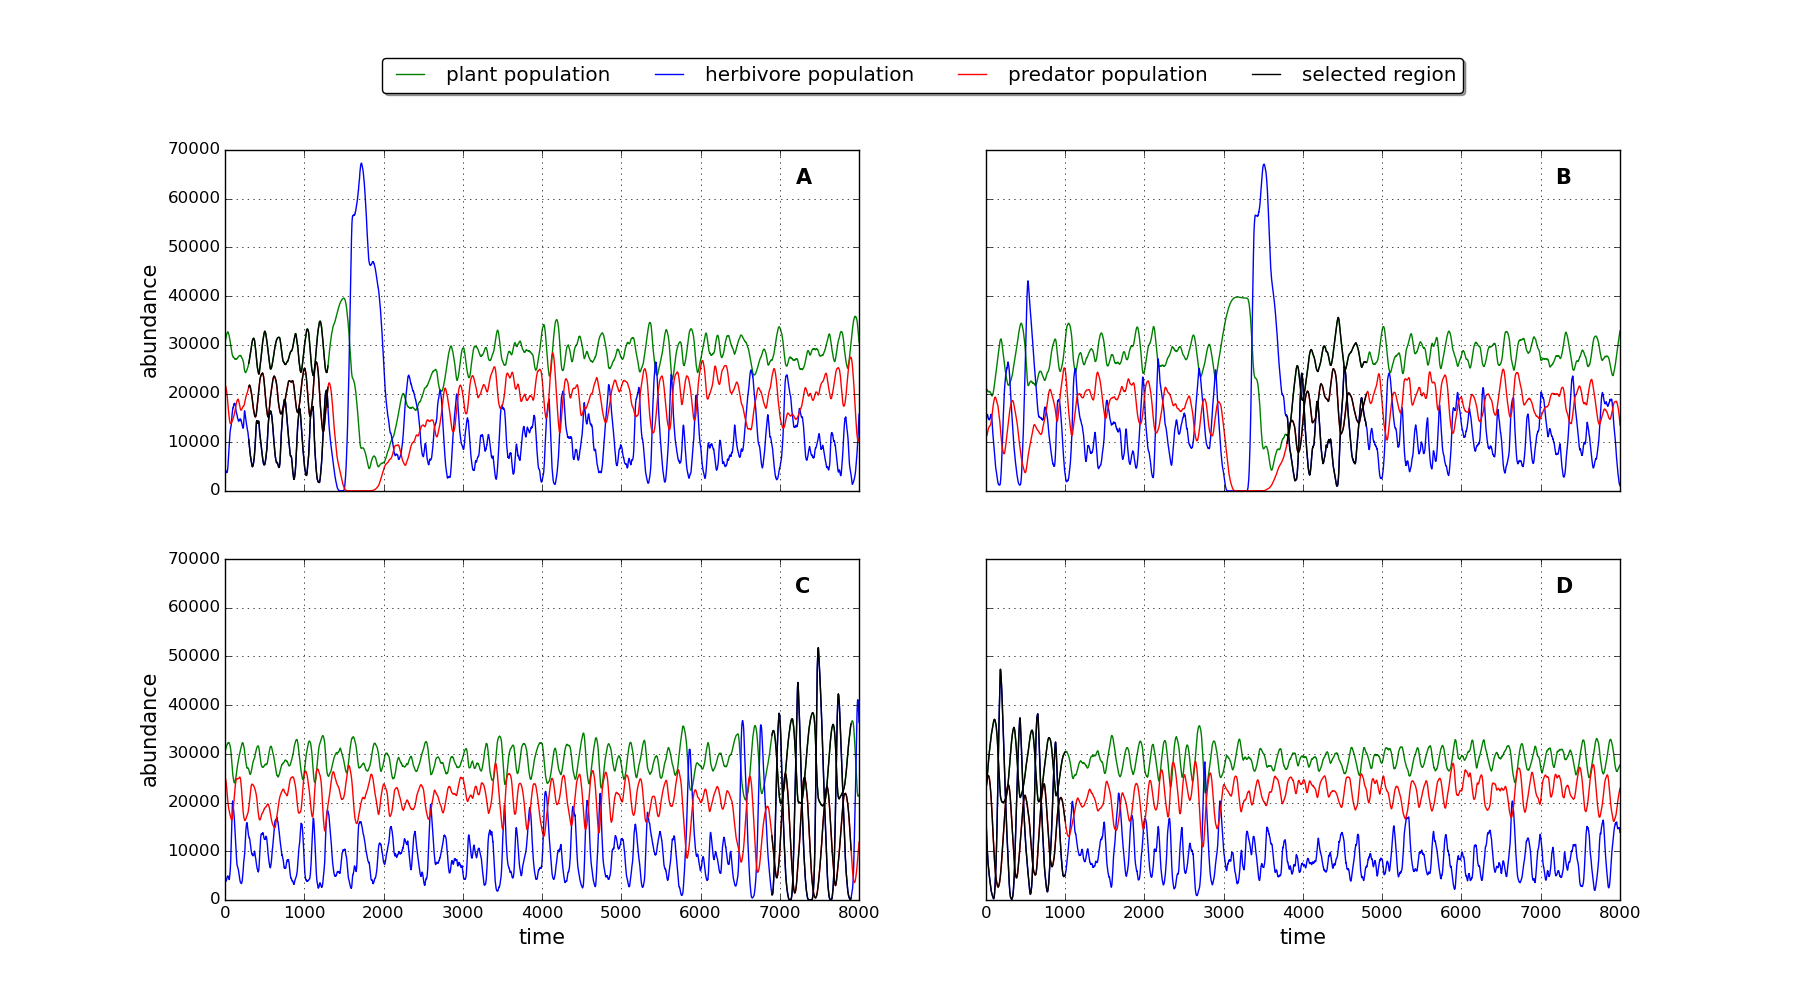
\includegraphics[width=\textwidth]{{{figures/IBM/3species/example_dynamics_3sp}}}
	\caption[Three species IBM dynamics.]{\textbf{Example dynamics of 3 species IBM} food chain, four different simulations (panels A,B,C,D). Top row: low IR ($10^{-5}$). Bottom row: high IR ($10^{-4}$). Regions plotted in black are those selected as \emph{data streams} for GLV fit (see text for details of how selected).}
	\label{fig:3sp_dynamics}
\end{figure}

Looking at the simulated food chain dynamics in figure \ref{fig:3sp_dynamics}, we speculate that the lack of convergence, and possibly the spurious interaction, may result from features of the dynamics. The dynamics shown are highly variable and appear \emph{quasi-periodic}. It may be that the GLV struggles to fit to large regions of such dynamics. In an attempt to overcome this problem we employ a method to select the optimum region of the dynamics for fitting the GLV. The selection method consists of scanning a sampling window of length 1000 time steps along the full dynamics. The model M0 is fitted to the dynamics within the window and the error functions (equation \eqref{eq:timme11}) of the three species are summed. We then select the window with the minimum total error in the fit. These selected regions are plotted in black for the four simulations shown in figure \ref{fig:3sp_dynamics}. The regions appear to share the common feature that they display oscillations of a relatively constant amplitude and period, compared to the rest of the dynamics. This observation supports our belief that the complexity of the dynamics negatively affects the GLV fit. In the analysis that follows all models are fitted to regions of the dynamics selected in the way just described.


%\begin{figure}
%	\centering
%	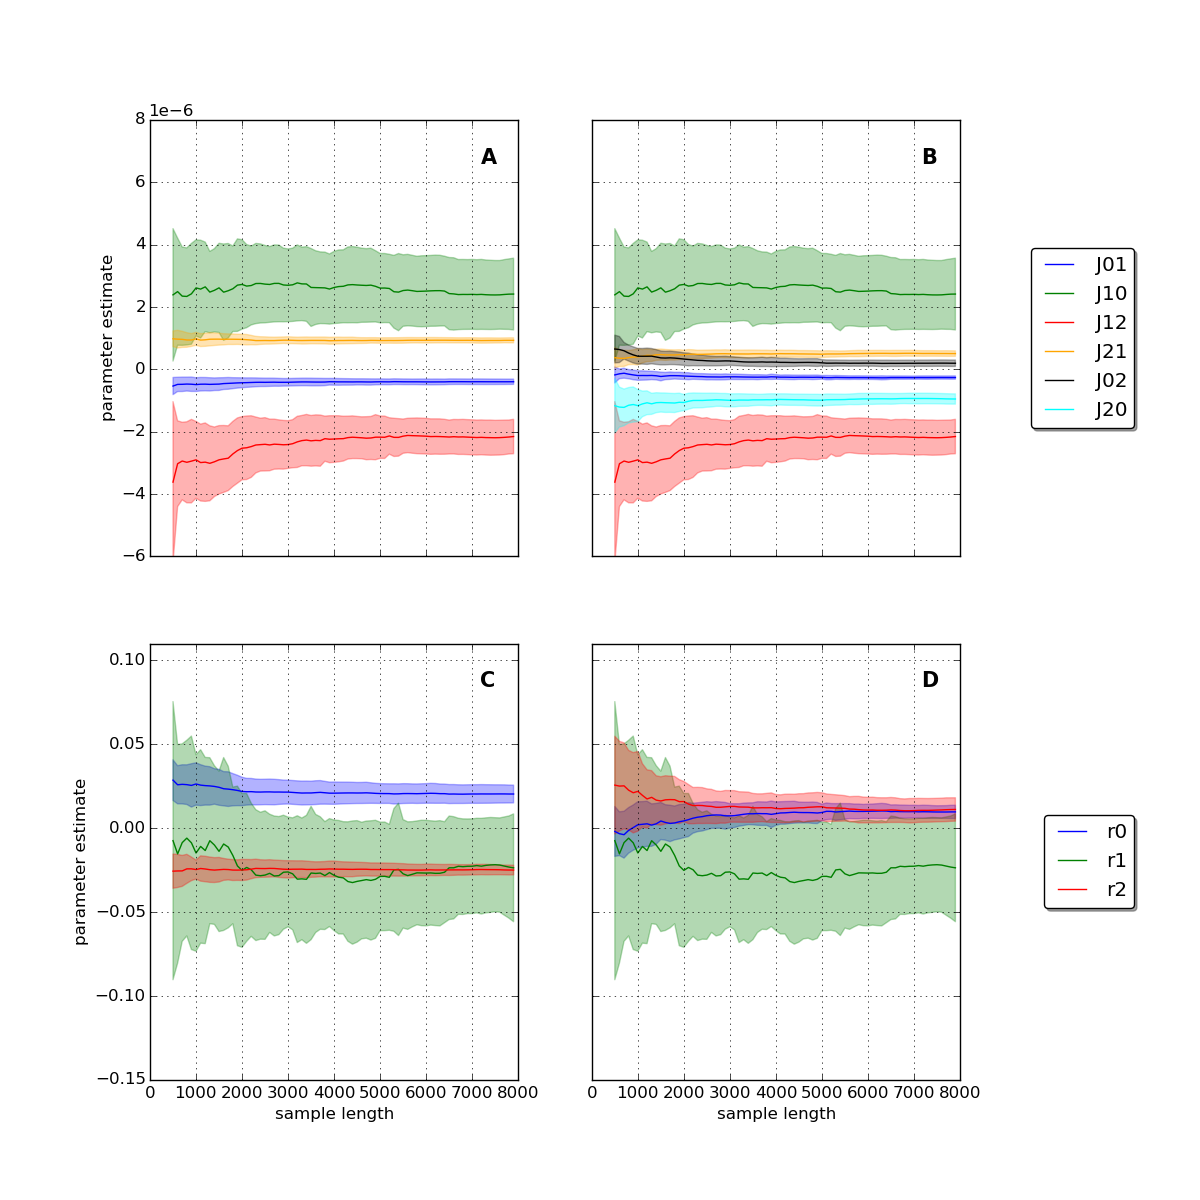
\includegraphics[width=\textwidth]{{{figures/IBM/3species/convergence_3sp_length_lowIR}}}
%	\caption{Convergence of estimates. 3 species.}
%	\label{fig:3sp_convergence_LI}
%\end{figure}

\begin{figure}
	\centering
	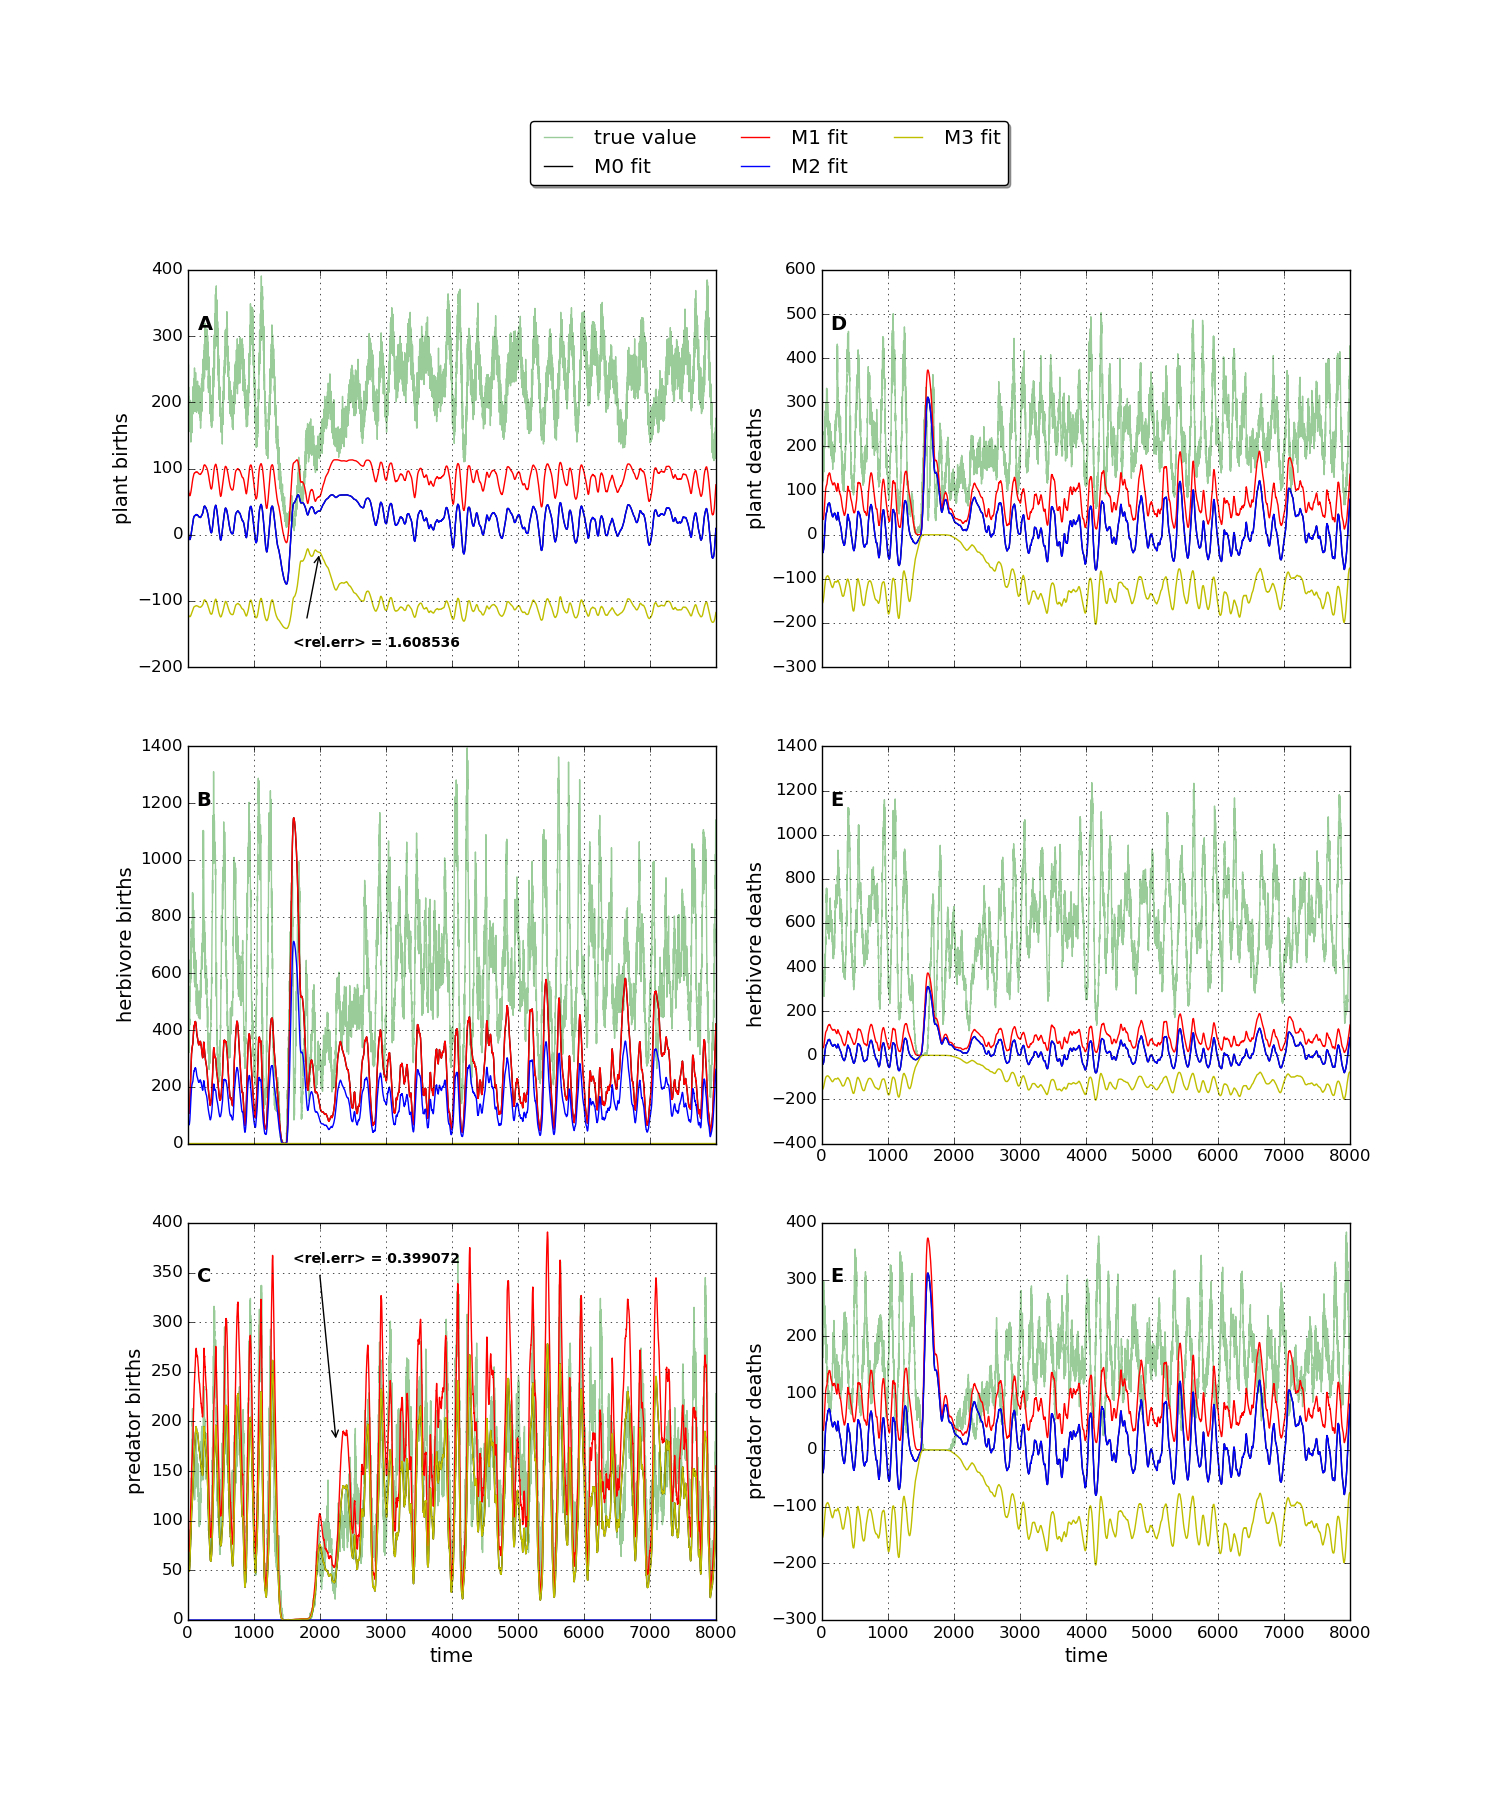
\includegraphics[width=\textwidth]{{{figures/IBM/3species/rate_estimates_3speices_li}}}
	\caption[Demographic rate predictions, three species, low IR.]{Similar to figure \ref{fig:rate_estimates_2sp_li}, but with different models fitted to a three species simulation at \textbf{low IR}. The simulation is the same as that in panel A of figure \ref{fig:3sp_dynamics}. The models M0-3 are depicted in figure \ref{fig:3sp_topo}. Arrows indicate the value of the relative error metric (RE) for two example model predictions.}
	\label{fig:rate_estimates_3sp_li}
\end{figure}

\begin{figure}
	\centering
	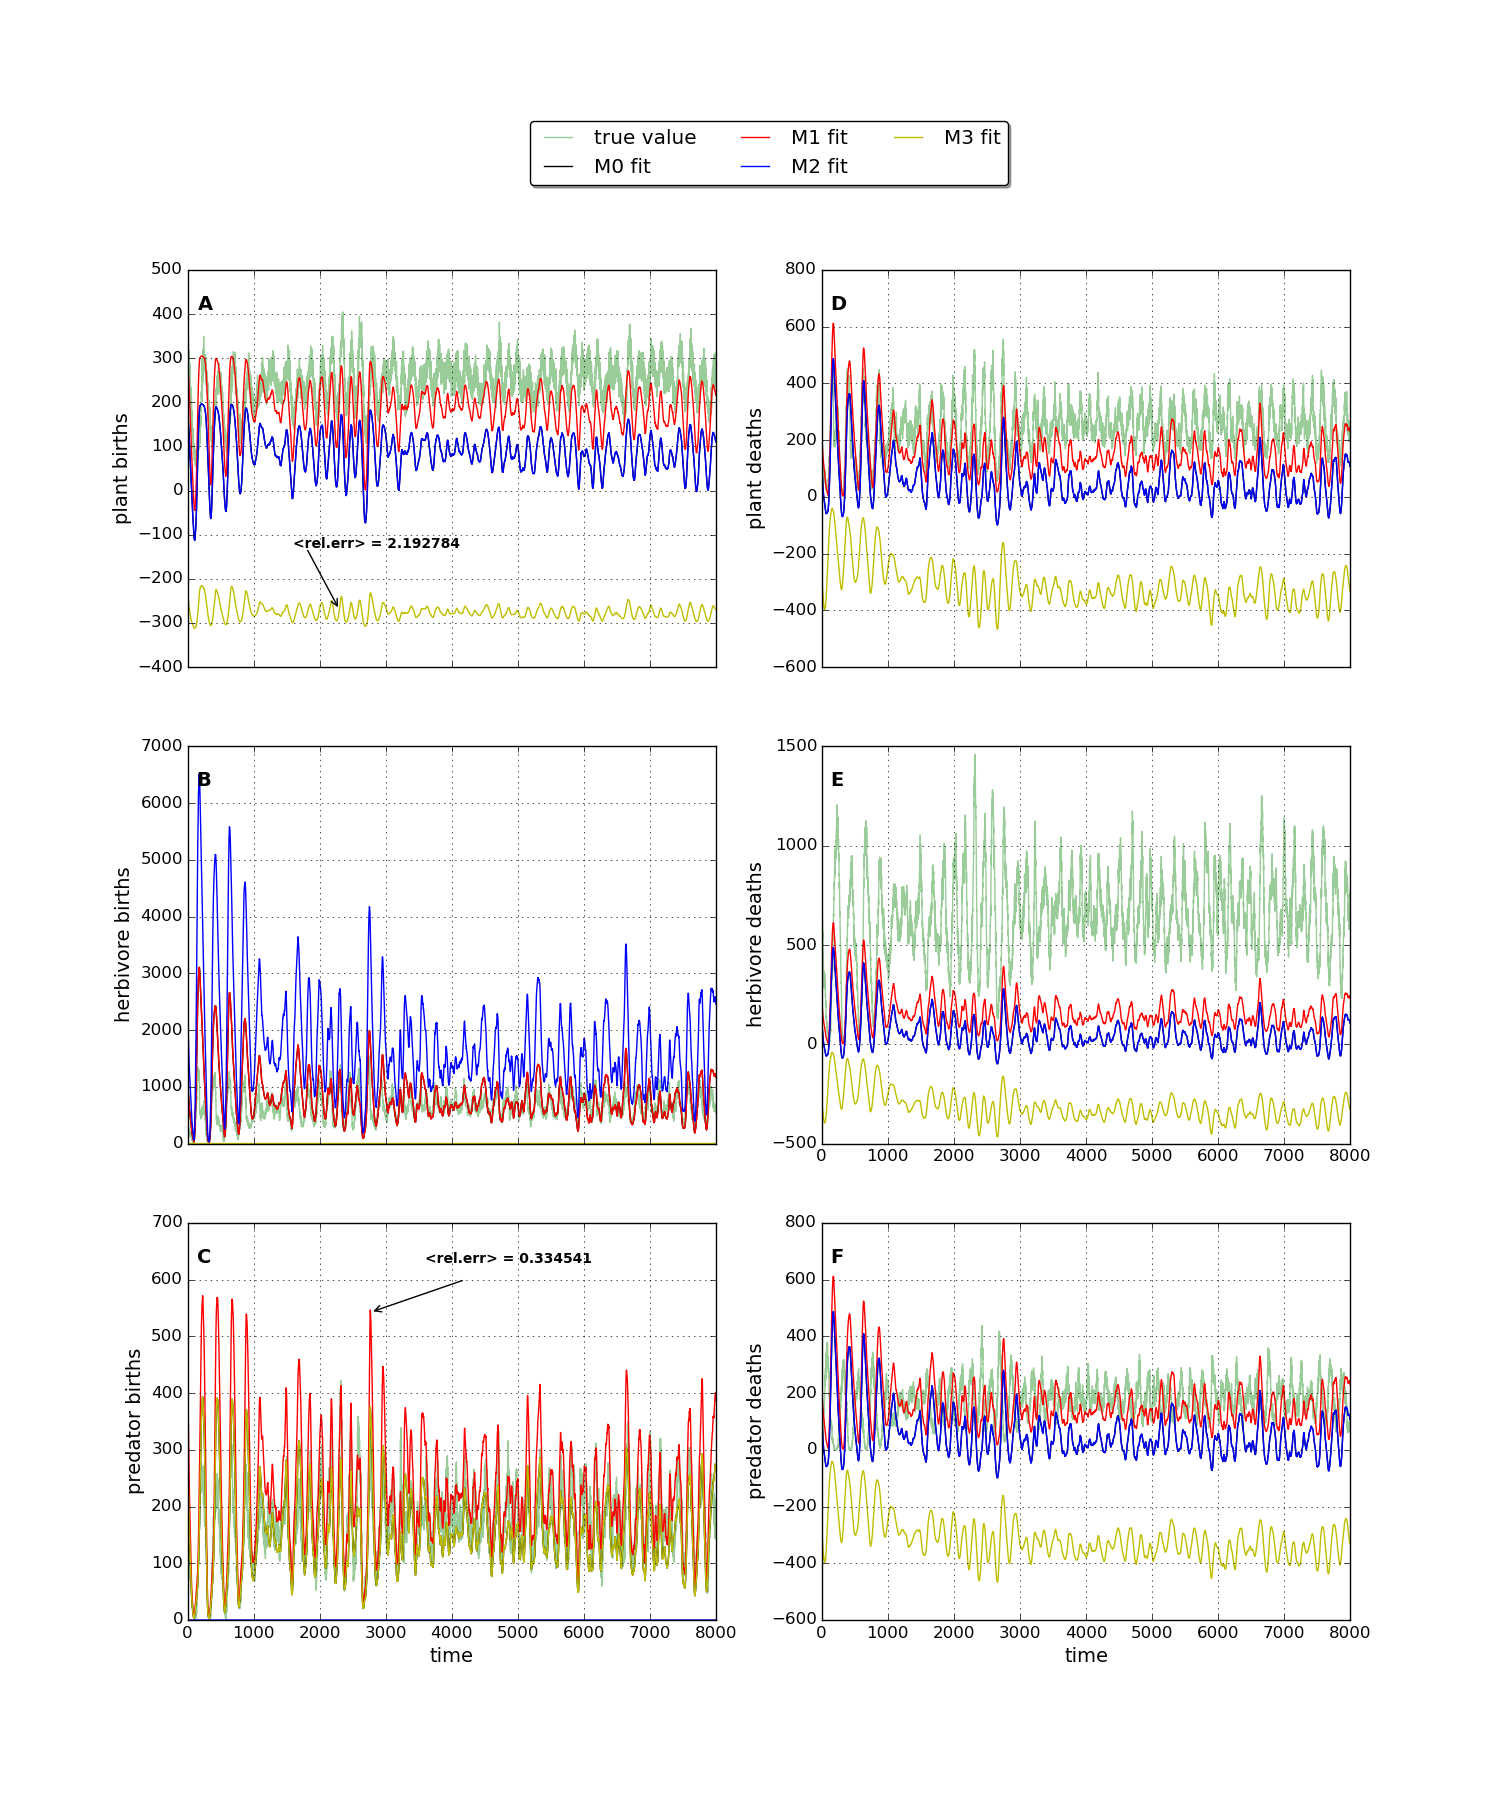
\includegraphics[width=\textwidth]{{{figures/IBM/3species/rate_estimates_3speices_hi}}}
	\caption[Demographic rate predictions, three species, high IR.]{Similar to figure \ref{fig:rate_estimates_3sp_li}, but for \textbf{high IR}. The simulation is the same as that in panel C of figure \ref{fig:3sp_dynamics}.}
	\label{fig:rate_estimates_3sp_hi}
\end{figure}

Figures \ref{fig:rate_estimates_3sp_li} and \ref{fig:rate_estimates_3sp_hi} show birth/death predictions of the fitted models to a single three species simulation at low IR and high IR respectively. Here we see significant difference between the quality of the predictions made by the different models. Note that for each species there is always a model (M1-3) that is equivalent to model M0 for that species. This is because in each of the models M1-3 one species is allowed to interact with both of the others, as they all are in model M0 (see figure \ref{fig:3sp_topo}). For most of the predictions at both IR values M3 (yellow) visibly performs the worst. This is the model with the link between plant and herbivore removed. Also M2 appears to perform worse than M1 in most cases. M2 is the model with the link between herbivore and predator removed. It is reassuring that the removal of links which are present in the true network results in predictions that are worse than those of M1. To confirm the repeatability of this observation we employ the relative error metric \eqref{eq:rel_er_rate_2sp} from the previous section, the determine the accuracy of model predictions over ensembles of 25 replicate simulations.

%% plotted at uni with:
%/MyFiles/cm1788/Documents/final_chapter/clean_analysis/3species/bc3_results/no_hl/lowIR/plot_rate_error_boxes
\begin{figure}
	\centering
	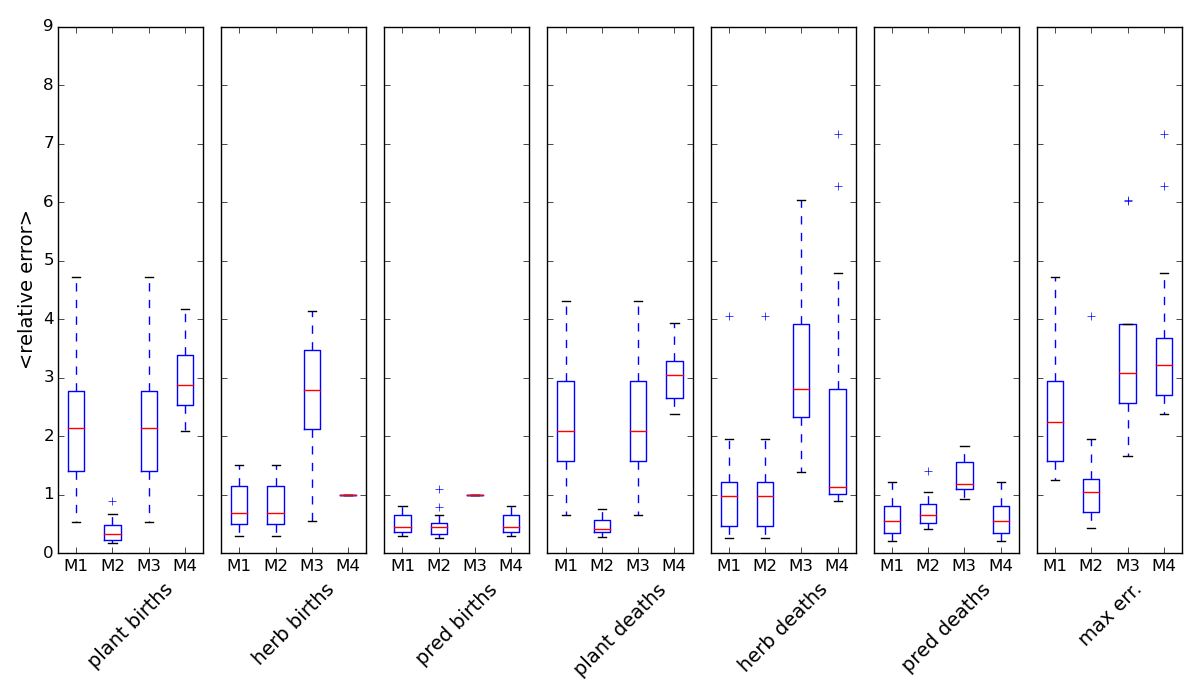
\includegraphics[width=\textwidth]{{{figures/IBM/3species/estimate_quality_3sp_LI}}}
	\caption[Relative error in three species predictions, low IR.]{Similar to figure \ref{fig:quality_2sp_li}, but with different models fitted to 25 three species simulations at \textbf{low IR}. This figure includes an additional statistic labelled \emph{max err.}, which is the maximum relative error in any prediction for a given simulation.}
	\label{fig:estimate_quality_3sp_LI}
\end{figure}
\begin{figure}
	\centering
	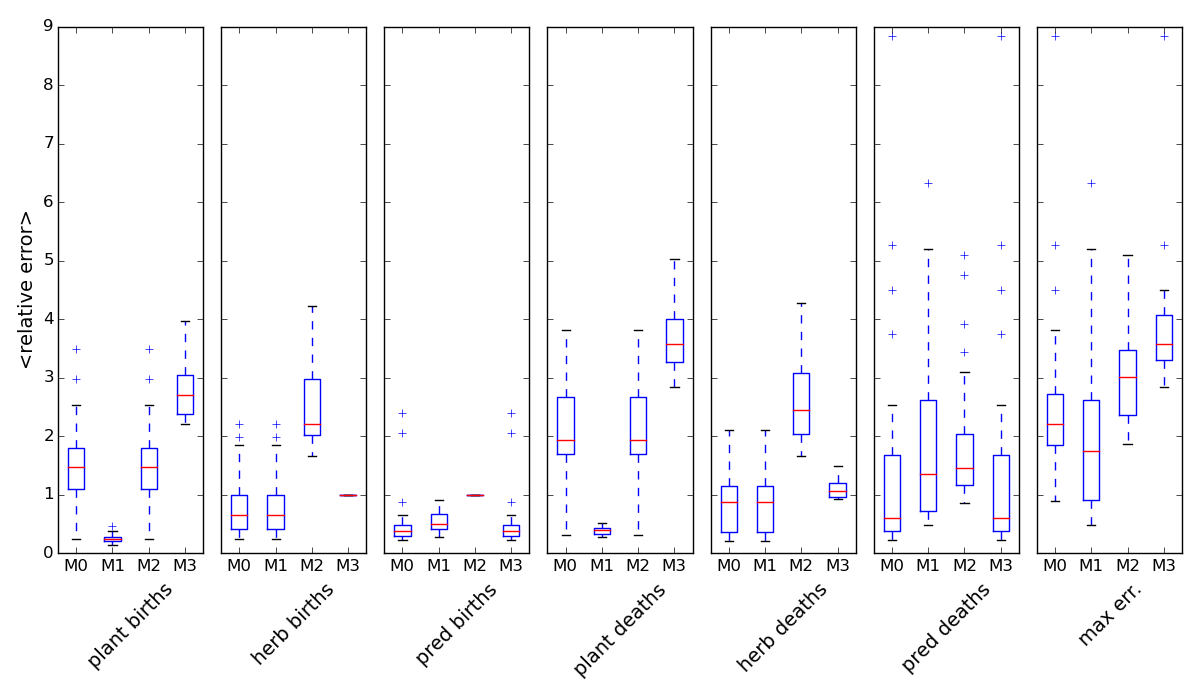
\includegraphics[width=\textwidth]{{{figures/IBM/3species/estimate_quality_3sp_HI}}}
	\caption[Relative error in three species predictions, high IR.]{Similar to figure \ref{fig:estimate_quality_3sp_LI}, but for 25 simulations at \textbf{high IR}.}
	\label{fig:estimate_quality_3sp_HI}
\end{figure}

Figures \ref{fig:estimate_quality_3sp_LI} and \ref{fig:estimate_quality_3sp_HI} show the relative errors in birth/death predictions for the ensembles of simulations at low and high IR respectively. We see that the predictions of M1 perform better than those of M2 and M3 in almost all cases (according to the median and the range of RE). Furthermore M1 performs at least as well as M0, the unconstrained GLV fit, is most cases. The exceptions to these observations are in the predator deaths at low IR, and both predator births and deaths at high IR. In these cases models M0 and M3 perform at either better than, or equally as well as M1. We conclude that the inclusion of the spurious link between plant and predator species improves the prediction of the demographic rates of the predator by the fitted model. We also reiterate that when this link is included the parameter estimates $\hat{J}_{02}$ and $\hat{J}_{20}$ suggest that the predator is being eaten by the plant (see for example figure \ref{fig:3sp_convergence_HI}). We return to this strange feature of the results in section \ref{sec:phase_space}. In the final panel of figures \ref{fig:estimate_quality_3sp_LI} and \ref{fig:estimate_quality_3sp_HI} we include the statistic \emph{maximum error}, which is the largest relative error out of all rate predictions for a given simulation. For example, in figure \ref{fig:rate_estimates_3sp_hi}, the maximum relative error for M3 is in the prediction of plant births. The error takes a value of 2.19, which is indicated by the arrow. The \emph{maximum error} statistic allows us to determine which model fit provides the best predictions across all demographic rates. In both the low and high IR cases M1, the model with the correct topology, performs the best.

% Not informative.
%\begin{figure}
%	\centering
%	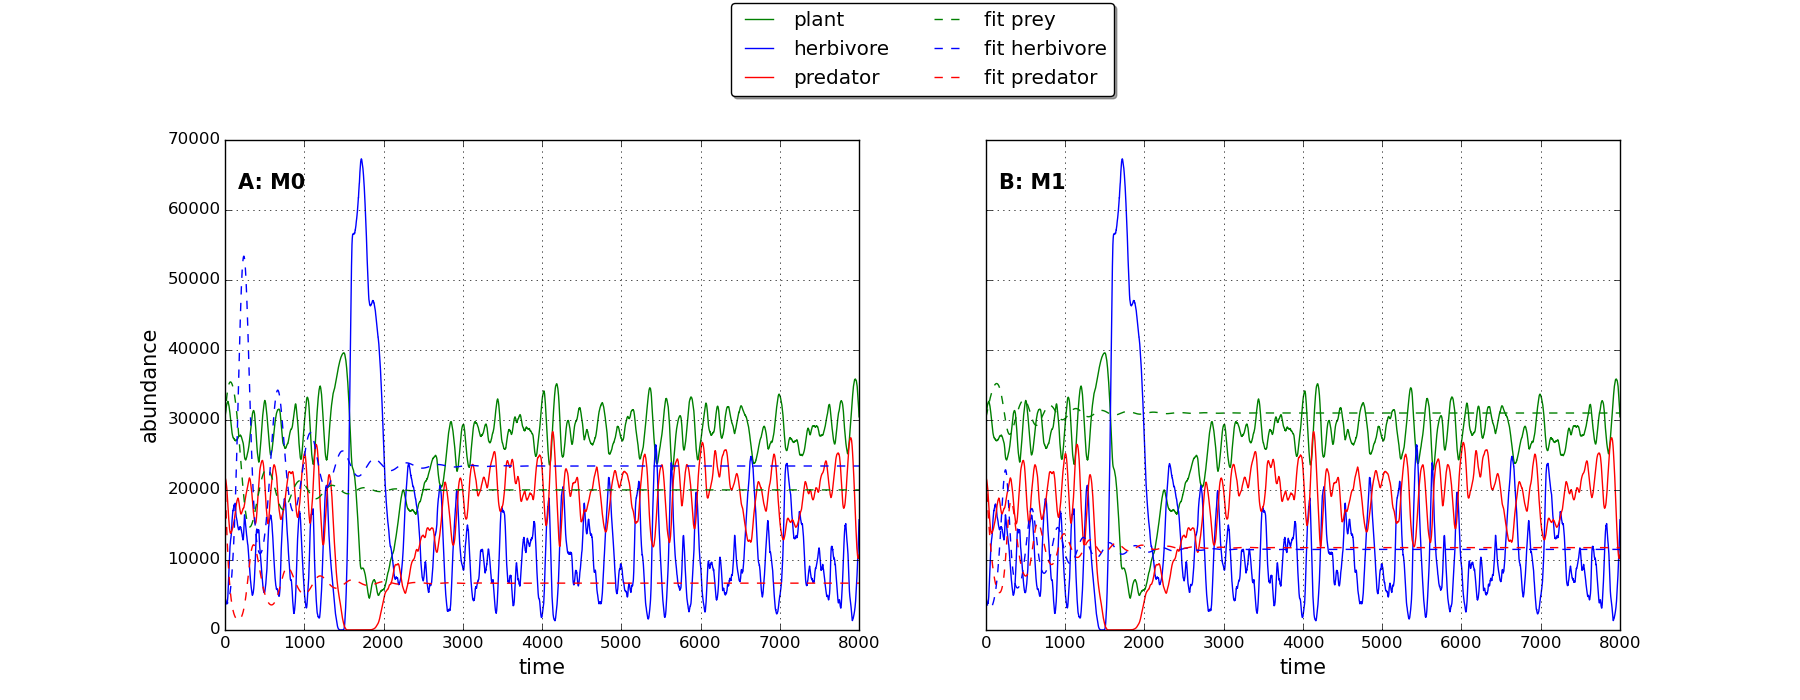
\includegraphics[width=\textwidth]{{{figures/IBM/3species/inferred_dynamics_3sp}}}
%	\caption{Fitted dynamics. }
%	\label{fig:inferred_dynamics_3sp}
%\end{figure}

\begin{figure}
	\centering
	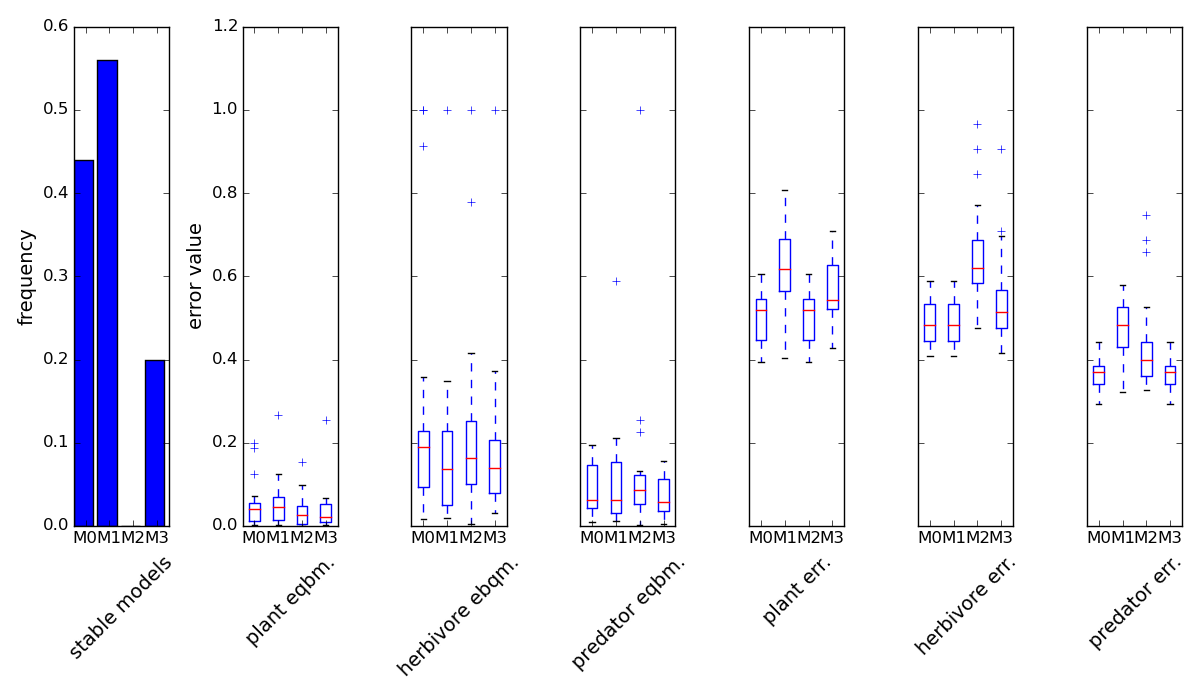
\includegraphics[width=\textwidth]{{{figures/IBM/3species/stability_and_error_3sp_LI}}}
	\caption[Model selection, three species, low IR.]{\textbf{Evaluating the performance of the different model fits} over 25 replicate simulations at \textbf{low IR}. Stability (panel 1) is determined from the Jacobian of the fitted model (see text). The errors in the equilibrium of each species (panels 2-4) represent the relative error between the equilibrium population of the fitted model and the long term average of the species population dynamics. The final three errors (panels 5-7) are the normalised error function of the model fit for each species (see text).}
	\label{fig:stability_and_error_3sp_LI}
\end{figure}

\begin{figure}
	\centering
	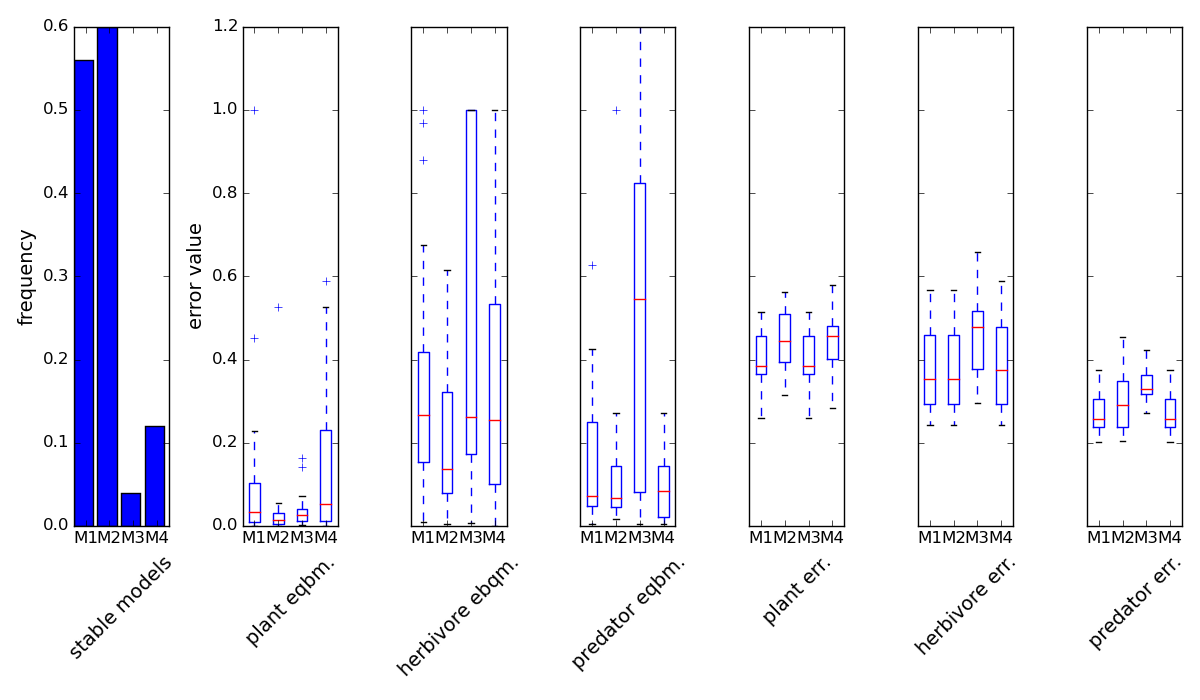
\includegraphics[width=\textwidth]{{{figures/IBM/3species/stability_and_error_3sp_HI}}}
	\caption[Model selection, three species, high IR.]{Similar to figure \ref{fig:stability_and_error_3sp_LI}, but for \textbf{high IR}.}
	\label{fig:stability_and_error_3sp_HI}
\end{figure}

The correct model (M1) may produce the best rate predictions, but without knowledge of the true rates we cannot use this fact to identify the correct topology. We now attempt to identify which model (M0-4) represents the correct topology using only knowledge of the fitted models, and information about the IBM population dynamics (i.e. no knowledge of true demographic rates). We conduct three checks on the fitted models. First we evaluate the Jacobian of the model and determine if the equilibrium is locally stable (see section \ref{sec:models}). Secondly we calculate the relative error between the model equilibrium and the long term average of the population dynamics for each species. Thirdly we compute the error function of the model fit $E(\hat{J}_i)$ for each species $i$ (equation \eqref{eq:timme11}), normalised by the sum of the first derivatives of the population dynamics of species $i$\footnote{This explanation is not clear, and does not justify the use of this measure}. The results of these three checks are summarised in figures \ref{fig:stability_and_error_3sp_LI} and \ref{fig:stability_and_error_3sp_HI} for the low and high IR ensembles respectively. At low IR, M1 does not perform consistently better than the competing models in terms of either equilibrium or error function values. At high IR, M1 performs best in terms of the predicted equilibrium values for all species, although the predator equilibrium results are comparable to those of M3. However M1 again does not display the lowest error function value for any species. In both the low and high IR cases the fitted M1 model is stable more frequently that any other. M0 is also stable with relatively high frequency, compared to M2 and M3 which are usually unstable. If presented with a single \emph{data stream} of three species from which to infer the correct interaction topology, it may be possible to do so with reasonable confidence based on these results (with particular focus on stability). However no conclusive method for doing so emerges from the three checks presented. We concluded that the identification of the correct topology from three species food chain simulations remains an open problem.

%% TOD DISCUSS RE IBM APPLICATION:

% > could introduce non-linearities to IS. E.g. hanlding time?
% > discuss application to larger system. Functional groupings...etc.
%
%\clearpage
\subsection{Five species results}
\label{sec:5sp_res_ibm}

In this section we briefly consider the application of the inference method to a five species system. The step from three to five species significantly increases the complexity of the problem. Given the difficulty of identifying the correct interaction topology for three species, we may anticipate that it is not possible with five. However, based on the three species results, we may expect reasonable predictions of demographic rates, especially when the fitted model is constrained to the correct topology (this constrained model is again called M1). With five species there are a total of ten possible inter-specific interactions. This fully connected topology is shown as M0 in figure \ref{fig:5sp_topo}. There are a combinatorially large number of subsets of M0, depending on how many links L are included. For a network with L links there are ${10 \choose L}$ distinct interaction topologies. For the IBM simulations we choose a symmetrical network with four links, shown as M1. It was experimentally determined that the symmetry of this network promoted stability in the population dynamics (results not shown). For example the introduction of the link $\hat{J}_{03}$ to M1 makes the network asymmetric, benefiting species 3 over species 1 (two feeding links versus one), and benefiting species 2 over species 0 (one predator versus two). The network M1 contains two plants (species 0 and 2), two herbivores (species 1 and 3) and a single predator (species 4).

\begin{figure}
\centering
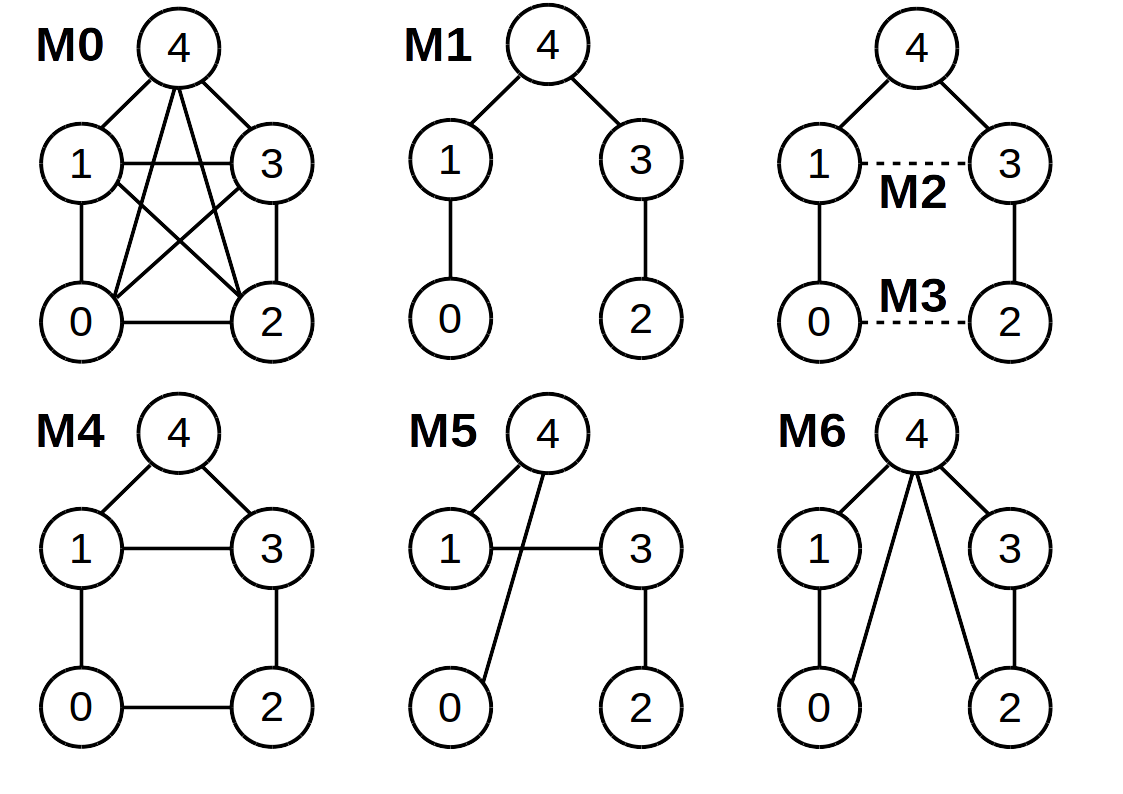
\includegraphics[width=0.5\textwidth]{{{figures/5sp_topologies}}}
\caption[Competing topologies, five species.]{Seven candidate 5 species models. M0: fully connected. M1: the true topology of the IBM simulations to which the GLV is fitted. M2 and M3: One link added to M1, as indicated. M4-6: Different but plausible topologies. All models include intra-specific interactions (self-loops), although these are not drawn.}
\label{fig:5sp_topo}
\end{figure}

\begin{figure}
	\centering
	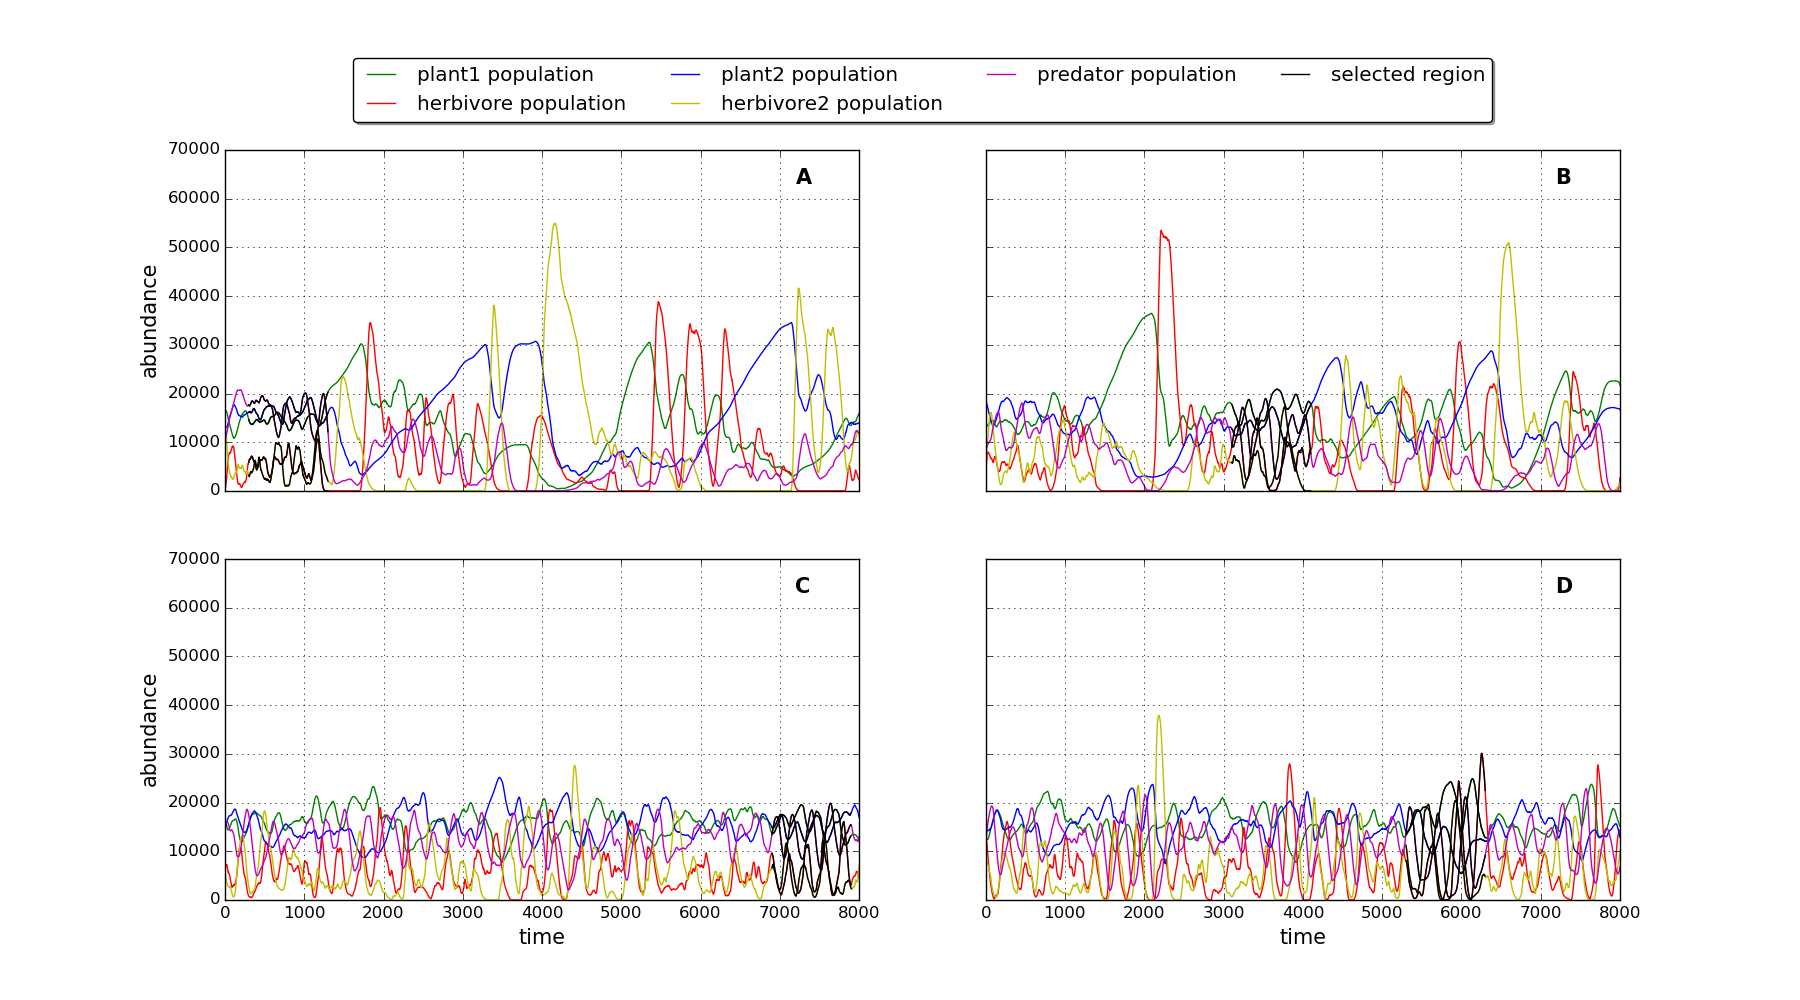
\includegraphics[width=\textwidth]{{{figures/IBM/5species/example_dynamics_5sp}}}
	\caption[Five species IBM dynamics.]{Similar to figure \ref{fig:3sp_dynamics}, but for five specie simulations of the IBM with interaction topology M1 (shown in figure \ref{fig:5sp_topo}). Panels A and B: low IR. Panel C and D: high IR. The regions plotted in black represent selected \emph{data streams} to which the GLV is fitted (selected using same criteria as in section \ref{sec:3sp_res_ibm}).}
	\label{fig:5sp_dynamics}
\end{figure}

Five species IBM dynamics with interaction topology M1 are shown in figure \ref{fig:5sp_dynamics}. Panels A and B show dynamics at low IR, which are more variable than the high IR dynamics shown in panels C and D. In what follows we focus on the high IR case based on previous observations that it is easier to fit to dynamics that are less complex. This choice reflects an attempt to slightly simplify the challenge posed by the inference of interactions from the 5 species system. We again select the optimum region of 1000 time steps from the dynamics to use as the data stream. The regions are selected in the same way as in section \ref{sec:3sp_res_ibm}, and are illustrated in figure \ref{fig:5sp_dynamics}. In this analysis we focus on the seven models depicted in figure \ref{fig:5sp_topo}. M0 is the full unconstrained GLV topology, while M1 is the true topology as discussed. The other models are selected as plausible alternatives to M1. In particular, the models M2-4 represent the true topology with the addition of one or two links between species in the same trophic level. These additions are plausible given the evidence of competition for space that we have seen previously (chapter \ref{chap:stress_testing}). As such we may expect these additional interactions to represent competitions (see section \ref{sec:av_inf_j}). 

\begin{figure}
	\centering
	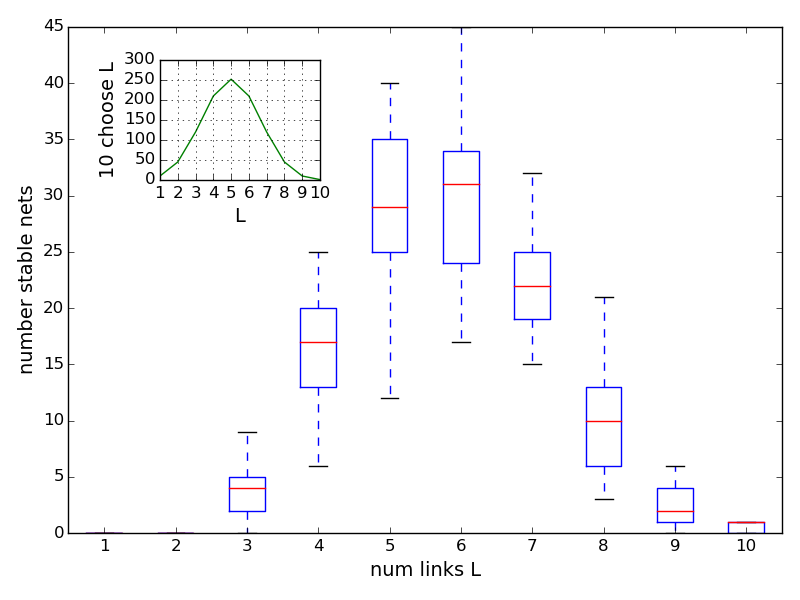
\includegraphics[width=\textwidth]{{{figures/IBM/5species/highIR_num_stable_nets}}}
	\caption[Number of stable five species topologies.]{\textbf{The number of stable 5 species topologies} with L inter-specific interactions, when fitted to 25 replicate IBM simulations at \textbf{high IR}. The IBM simulations use topology M1 (figure \ref{fig:5sp_topo}), which has L$=4$. The inset shows the total number of possible networks with L links, all were tested. Stability is defined as the local stability of the equilibrium of the fitted model.}
	\label{fig:5sp_stable_nets}
\end{figure}

Given the large number of possible topologies we first study the stability properties of all the potential competing models. Figure \ref{fig:5sp_stable_nets} summarises how many stable models exist at each value of L, for all 25 repeat simulations. Stability is again defined by the Jacobian of the fitted models. The number of stable models varies with L in a manner the approximately matches the total number of possible models (shown as an inset in the figure). However the most possible models exist at $L=5$,  whereas the greatest number of stable models exist at $L=6$. The true model M1 contains four links. At this value of L there are $10 \choose 4 = 210$ possible models, of which only between 5 and 25 are dynamically stable. This raises the question as to whether M1 belongs to the stable set of models with $L=4$. Figure \ref{fig:5sp_stable_models} shows the frequency with which each model M0-6 is stable over the 25 replicates. We see that M1 is stable in all 25 cases, as are M2, M3 and M4. The latter models represent M1 with addition of either one or two links between species in the same trophic level (plant-plant, herbivore-herbivore, or both). We discuss the frequent stability of these three models further in section \ref{sec:si_discussion}. Model M0 is stable in around half of the simulations, while models M5 and M6 are rarely stable. Therefore it appears that focus on dynamics stability can indeed reduce the search space for identification of the correct topology, especially if the number of links in the true network is known.

\begin{figure}
	\centering
	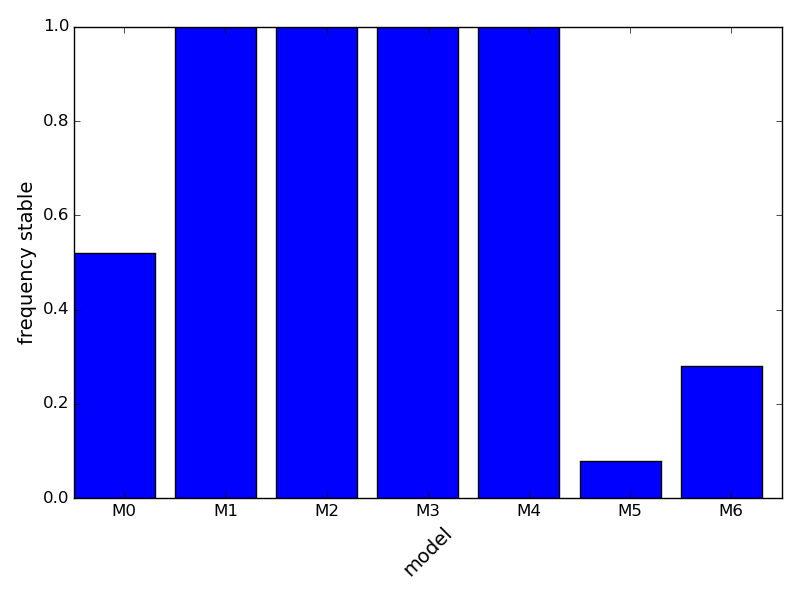
\includegraphics[width=\textwidth]{{{figures/IBM/5species/highIR_stable_models}}}
	\caption[Frequency of stability for competing five species topologies.]{\textbf{The frequency with which each model (M0-6) is stable} when fitted to 5 species dynamics at \textbf{high IR} (25 replicate simulations). Stability is defined as the local stability of the equilibrium of the fitted model. The models M0-6 are shown in figure \ref{fig:5sp_topo}.} 
	\label{fig:5sp_stable_models}
\end{figure}

%% These are not included because we cannot choose the right model with 3 species even.
%\begin{figure}[p]
%	\centering
%	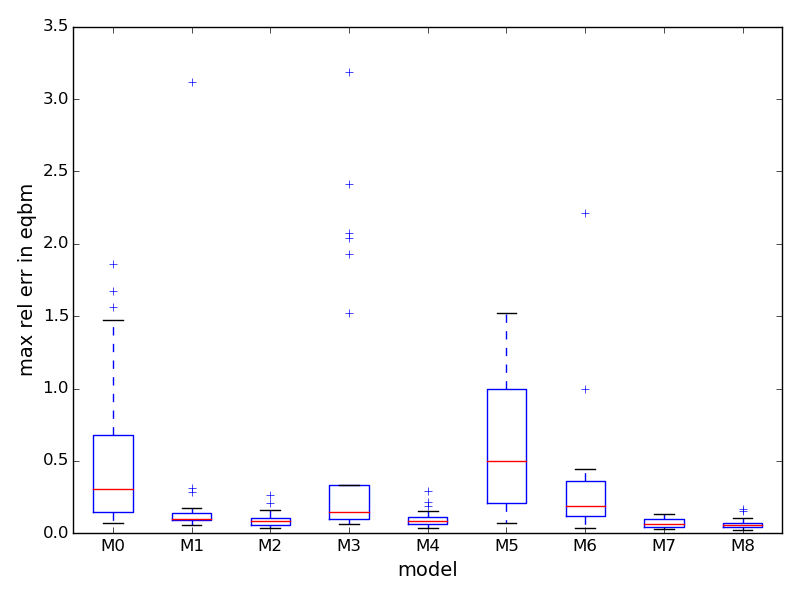
\includegraphics[width=\textwidth]{{{figures/IBM/5species/highIR_eq_err}}}
%	\caption{5 species: error in equilibrium}
%	\label{fig:5speqerr}
%\end{figure}
%
%\begin{figure}[p]
%	\centering
%	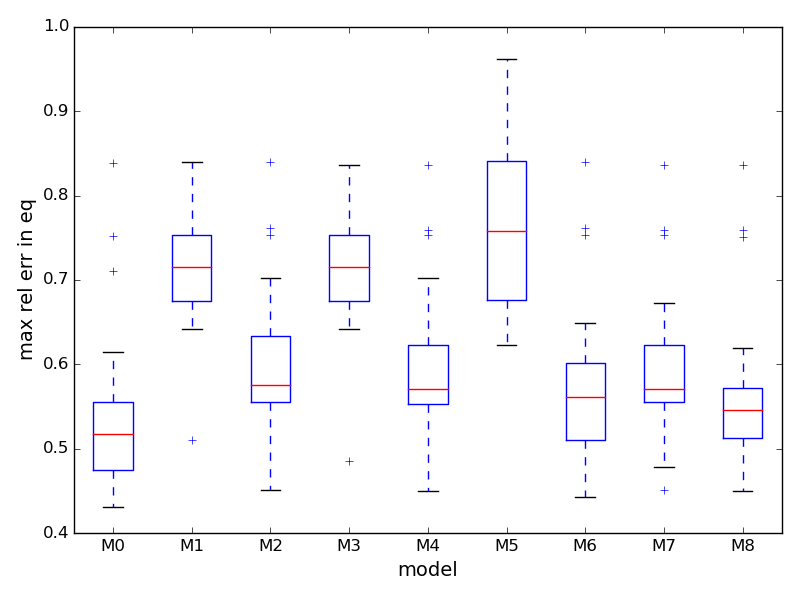
\includegraphics[width=\textwidth]{{{figures/IBM/5species/highIR_errfn}}}
%	\caption{5 species: error in gradient fit function}
%	\label{fig:5sp_errfn}
%\end{figure}

\begin{figure}
	\centering
	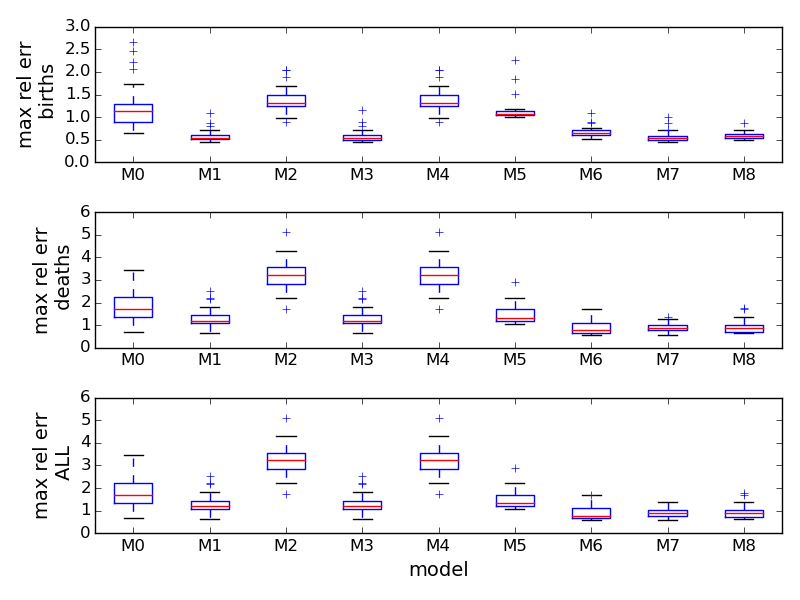
\includegraphics[width=\textwidth]{{{figures/IBM/5species/highIR_rate_errors}}}
	\caption[Five species demographic rate predictions.]{\textbf{Relative errors in the demographic rate predictions} of the models M0-6 (figure \ref{fig:5sp_topo}), plus two additional models: M7 and M8. M7 is selected as the model in the set of stable models with four links (L$=4$) that has the lowest relative error. M8 is the same but for L$=5$. As such the topologies of M7 and M8 are not fixed. The errors shown are the maximum relative error in the predicted births (top row) and predicted deaths (middle row) for each simulations, and the maximum relative error in all rate predictions (bottom row). Relative error is defined in equation \eqref{eq:rel_er_rate_2sp}, and example rate predictions for three species are illustrated in figure \ref{fig:rate_estimates_3sp_li}.}
	\label{fig:5s_rate_errors}
\end{figure}

Figure \ref{fig:5s_rate_errors} summarise the relative errors in the demographic rate predictions for the seven models M0-6, and an additional two models. These models, M7 and M8, are selected on a case by case basis from the set of stable models with L$=4$ and L$=5$ respectively. The models are selected such that the maximum relative error in any rate prediction is minimised. Therefore the topology of these models can vary between simulations. From the figure we observe that, on aggregate, the predictions of M1, M3 and M5 are of comparable quality. The models M6-8 perform better, but only slightly. All models have a median maximum relative error (bottom panel) that is approximately equal to or greater than one. Therefore none of the models give accurate rate predictions for all species. We acknowledge that some information is lost by the use of the maximum relative error metric. For example a model may produce very accurate predictions in all but one of the rates. Additionally we note that the use or greater L values increases the number degrees of freedom, and therefore is likely to improve fit of the constrained GLV. Therefore further analysis should employ more sophisticated techniques for model comparison, such as the \emph{Akaike information criterion} (AIC) \cite{aho2014model}. In general we conclude that the true model (M1) performs favourably compared to competing alternative models in terms of stability and rate predictions. However no consistent criteria for the selection of the correct network topology have been identified.  
%\clearpage
%\begin{figure}[p]
%	\centering
%	\includegraphics[width=\textwidth]{{{figures/IBM/5species/highIR_fitted_FR}}}
%	\caption{5 species: functional response (High IR)}
%	\label{fig:5sp_FR_fit_highIR}
%\end{figure}
%
%\begin{figure}[p]
%	\centering
%	\includegraphics[width=\textwidth]{{{figures/IBM/5species/lowIR_fitted_FR}}}
%	\caption{5 species: functional response (Low IR)}
%	\label{fig:5sp_FR_fit_lowIR}
%\end{figure}

%\clearpage
%\section{Discussion}
%\label{sec:discussion}
%
%Points referenced in text above, make sure to discuss them!..
%
%\begin{itemize}
%	\item Discuss how this methodology could be used on empircal data...
%	\item Limitations of ODE models (non-spatial, repsonse to debate on FR)
%	\item Possibility of extending to more than two specie systems (if this is actually done then change ref in text above)
%	\item discussion of other forms of FR (not H) - or disucssed already in inro?
%	
%	\item good GLV fit to LV even with 100 sample points - realistic?
%	
%	\item how good is the method of model fitting. Discuss more computationally expensive options (mentioned in section on Timme method)
%	
%	\item Spatial heterogeneity - we do not explore this here, but acknowledge that it represents are source of error. Gives example in extremis - 2 species only interacting on boundary. Also we know that there is some level of spatial aggregation, especially at low IR - possibly show one plot of this?
%	
%	\item Could introduce prey handling to IBM to create non-linear FR.
%	
%	\item Our method could be used to pick out coupling to other variables e.g evironmental (temperature) if expressed in a certain way.
%	
%	\item In real application would not have luxury of selecting the section of time series with best fit! Would be lucky to have 1000 time points at all! 
%\end{itemize}
%
%

\subsection{Inferred topologies}
\label{sec:av_inf_j}

We now explicitly consider the accuracy of the inferred topologies when fitting the full (unconstrained) GLV model to data generated by the IBM model. That is, we ask whether the inferred interaction strengths correctly identify which species are interacting and how they are interacting. Here we plot the inferred topologies, and compare them to the true interaction networks used in the IBM simulations. We analyse a 5 species system, and 60 species systems with and without mutualism. In the case of 60 species the complexity of the problem is reduced by aggregating the population dynamics. The time series for all species belonging to each functional group are summed. As such the 60 species system without mutualism produces four groups: one for each trophic level. The 60 species system with mutualism produces six groups: two in the lowest two trophic levels, and one in the top two levels. The GLV model is then fitted by treating each of the groups as a single \emph{species}. In all the results presented the GLV is fitted to a sample of 1000 time steps, selected as before by scanning the time series for the region which produces the lowest error function value. We perform $K=25$ replicate simulations for each system and take the average value of the estimated interaction strengths $\langle \hat{J}_{ij} \rangle = \Sigma_{k=1}^{25} \hat{J}_{ijk} \quad \forall i,j $.

\begin{figure}
\centering
\includegraphics[width=\textwidth]{{{figures/IBM/5species/5species_average_Jhat}}}
\caption[Inferred topology, five species.]{\textbf{Five species system at high IR} (0.001). Panel A: The topology of the interaction network used for simulations. The links displayed are all of equal weight, since we do not specify interaction strengths prior to simulation, only the topology. Panel B: The average inferred topology over 25 replicate simulations. For each simulation the full GLV model is fitted to the optimum region of 1000 time steps (see text). We take the average value of each element of the inferred interaction matrix $\hat{J}$, over the 25 replicates. The links are coloured by the type of inferred interaction. If $\hat{J}_{ij}<0$ and $\hat{J}_{ji}>0$ this indicates a trophic link from resource $i$ to consumer $j$, plotted in black with the thick end twoards the consumer. If both $\hat{J}_{ij}<0$ and $\hat{J}_{ji}<0$ the link is competitive and plotted in red. If both $\hat{J}_{ij}>0$ and $\hat{J}_{ji}>0$ the link is mutualistic and plotted in blue. All links are weighted by the average interaction strength: $(\hat{J}_{ij}+\hat{J}_{ji})/2$.}
\label{fig:av_inf_j_5sp}
\end{figure}
%% plotted with: figures/IBM/exmple_networks_inferrence/5sp_test/5sp_plot_inf.py
%% which fits full GLV to stabres/best_bits from BC3.

Figure \ref{fig:av_inf_j_5sp} shows the results for the same 5 species system studied in section \ref{sec:5sp_res_ibm}, which was simulated here with IR$=0.001$. Panel A shows the interaction network used for the simulations, while panel B shows the average inferred topology obtained by the GLV fits. An inferred trophic link from species $i$ to species $j$ is identified as one for which $\hat{J}_{ij} < 0$ and $\hat{J}_{ji} > 0$. Such links are plotted in black, with the thick end of the line indicating the consumer. Competitive links are those for which both $\hat{J}_{ij} < 0$ and $\hat{J}_{ji} < 0$. Such links are plotted in red. All links are weighted by the logarithm of the average interaction strength, multiplied by a scaling factor: $ln(\gamma \times (\hat{J}_{ij} + \hat{J}_{ji})/2)$. Comparing panels A and B we see that the trophic links which \emph{are present} in the system, are correctly identified by the GLV fit (0-1, 2-3, 1-4, 3-4). Additionally the GLV identifies competitive interactions between the pair of plant species (0-2), and between the two herbivore species (1-3). Since we have previously seen evidence of competition for space in the IBM (chapter \ref{chap:stress_testing}), we may be confident that these inferred competitive interactions are meaningful. However the method also identifies four spurious interactions. Namely the plants are seen to consume all three non-basal species. Two of these links are weak (0-3, 1-2), but the other two are relatively strong (0-4, 2-4). We conclude that the method works well in this case, on average, other than the two strong trophic links form top-predator to the basal species. We return to this feature in section \ref{sec:phase_space}.

\begin{figure}
\centering
\includegraphics[width=\textwidth]{{{figures/IBM/60species/60species_orig_mut0_average_Jhat}}}
\caption[Inferred topology, sixty species without mutualism (1).]{Similar to figure \ref{fig:av_inf_j_5sp}, but for \textbf{60 species with MAI=0}. IR$=0.005$. Here each node represents a functional group. 0: Non-mutualistic plants. 1: Mutualistic plants. 2: Herbivores. 3: Mutualistic-animals. 4: Primary predators. 5: Top predators. Trophic links in black, competitive links in red, mutualistic links in blue.}
\label{fig:av_inf_j_60sp_orig_mai0}
\end{figure}
%% pltted with: figures/IBM/exmple_networks_inferrence/60sp_test/60sp_plot_inf.py
%% results calculated from original (ch3) sims using:
%% habitat_loss_project/IBM/random_results/chris_plots_python/scripts/av_inf_J.py

Figure \ref{fig:av_inf_j_60sp_orig_mai0} shows results for a 60 species system without mutualism (MAI=0). Again 25 replicate simulations were run, this time using the \emph{default parameter values}. These values were used to deliberately ensure a significant amount of noise was present in the simulations, resulting form the high immigration rate ($IR=0.005$). The nodes here represent the four functional groups: plants, herbivores, primary predators, and top predators. Panel A indicate the true interactions structure, and we see that here top predators can feed on plants (as in chapter \ref{chap:habitat_loss_high_immigration}). Panel B shows the average inferred network. We see that all trophic links are correctly identified, except for the link between herbivores and primary-predators (1-4). This links is inferred a competitive, which may be a reasonable inference to make. Not all primary-predators consume herbivores, and not only do these two groups compete for space, but some species within these groups also compete for resources. Figure \ref{fig:av_inf_j_60sp_new_mai0} shows results for the same 60 species system (MAI=0), but this time with the links between basal and top-predator species removed (as in chapter \ref{chap:varying_immigration_rate}). Again all trophic interactions are inferred correctly. The removed link (0-5) is identified as competitive, although it is weaker than the trophic links. There is no reason to think that basal species compete with top-predators. Therefore we conclude that this link is spurious. 

\begin{figure}
\centering
\includegraphics[width=\textwidth]{{{figures/IBM/60species/60species_new_mut0_average_Jhat}}}
\caption[Inferred topology, sixty species without mutualism (2).]{Similar to figure \ref{fig:av_inf_j_60sp_orig_mai0}, but for \textbf{60 species at MAI=0, without links between basal species and top-predators.}}
\label{fig:av_inf_j_60sp_new_mai0}
\end{figure}
%% pltted with: figures/IBM/exmple_networks_inferrence/60sp_test/60sp_plot_inf.py
%% results calculated from BC3 runs: original/... on BC3

\begin{figure}
\centering
\includegraphics[width=\textwidth]{{{figures/IBM/60species/60species_orig_mut0.5_average_Jhat}}}
\caption[Inferred topology, sixty species with mutualism (1).]{Similar to figure \ref{fig:av_inf_j_60sp_orig_mai0}, but for \textbf{60 species at MAI=0.5}.}
\label{fig:av_inf_j_60sp_orig_mai0.5}
\end{figure}
%% pltted with: figures/IBM/exmple_networks_inferrence/60sp_test/60sp_plot_inf_mut.py
%% results calculated from original (ch3) sims using:
%% habitat_loss_project/IBM/random_results/chris_plots_python/scripts/av_inf_J_mut.py

Figure \ref{fig:av_inf_j_60sp_orig_mai0.5} shows results for a 60 species system with mutualism (MAI=0.5). By including mutualism the number of functional groups is increased from four to six. In the bottom trophic level there are non-mutualistic (0) and mutualistic (2) plants. In the second trophic level there are herbivores (1) and mutualistic-animals (3). The green link in panel A indicates the mutualism between groups 2 and 3. Form panel B we see that the feeding relationships of the top two trophic levels (groups 4 and 5) are inferred correctly. However there is some confusion at the base of the food web. Specifically the plant-herbivore interaction (0-1) is inferred as competitive, and the non-mutualistic plants are inferred to consume the mutualistic animals. The mutualistic interaction (2-3) is identified as a trophic link, rather than a mutualism. However, this in not necessarily wrong since energy does flow along this pathway. As with the five species system, the method identifies competition between groups in the same trophic level (0-2 and 1-3). Figure \ref{fig:av_inf_j_60sp_new_mai0.5} shows results for the same 60 species system, but with the links between basal and top-predator species removed. This removal significantly affects the results, and numerous spurious interactions are identified. In particular, all but one of the inferred top-predator interactions are incorrect. The method does detect a strong signal of mutualism between groups 2 and 3. However, given the high level of error overall, this is not particularly encouraging. 

\begin{figure}
\centering
\includegraphics[width=\textwidth]{{{figures/IBM/60species/60species_new_mut0.5_average_Jhat}}}
\caption[Inferred topology, sixty species with mutualism (2).]{Similar to figure \ref{fig:av_inf_j_60sp_orig_mai0}, but for \textbf{60 species at MAI=0.5, without links between basal species and top-predators.}}
\label{fig:av_inf_j_60sp_new_mai0.5}
\end{figure}
%% pltted with: figures/IBM/exmple_networks_inferrence/60sp_test/60sp_plot_inf.py
%% results calculated from BC3 runs: original/... on BC3

\subsection{Phase space analysis}
\label{sec:phase_space}
%
One feature of the inference method, emerging from the analysis of systems with more than two species, is its tendency to detect spurious types of interaction between plant and predator species. In the three species case the estimated model parameters suggested that the predator was being eaten by the plant (figure \ref{fig:3sp_convergence_HI}). In the five species case the same phenomenon was observed (figure \ref{fig:av_inf_j_5sp}), and in the 60 species systems with mutualism the plants appeared to consume the mutualistic-animals (figures \ref{fig:av_inf_j_60sp_orig_mai0.5} and \ref{fig:av_inf_j_60sp_new_mai0.5}). In this section we propose an explanation for why the inference method produces these spurious results.

A robust feature of predator-prey dynamics, such as those modelled by the GLV, is that the oscillations of the predator population lag behind those of the prey population. This phase lag results in trajectories with anti-clockwise rotation in the phase plane, when the prey population is plotted on the x-axis, and the predator on the y-axis.  This feature has been used previously in attempts to infer predation interactions. For example Sandvik et al. \cite{sandvik2004using} developed a method to quantify the direction and extent of this rotation, in order to detect signatures of predation from empirical population dynamics. However in certain situations the phase relationship may be reversed. For example Gilpin showed that certain sections of the famous Hudson Bay hare-lynx time series display clockwise rotation in the phase-plane. This led to the playful title of his publication: `\emph{Do hares eat lynx?}' \cite{gilpin1973hares}. Various models have managed to produce predator-prey dynamics that display such clockwise rotation, for example by including \emph{time-delay} \cite{hsu1995global}, or rapid evolution \cite{cortez2014coevolution}. However it could be that the clockwise rotation results from other factors. The hare-lynx system is embedded in a larger food web \cite{stenseth1997population}. It may be that trophic interactions with other species are enough to disrupt the usually robust anti-clockwise rotation. Alternatively the dynamics may be disrupted by environmental forcing, which Mutshida et al. \cite{mutshinda2009drives} suggest has a stronger effect on population dynamics than trophic interactions in natural systems.

%In this section we discuss why we think the method is not working. We refer to various other studies that have observed reversed phase-relationships between predator and prey. We finish with a discuss of alternative methodologies that may be less vulnerable to this error.

\begin{figure}
	\centering 
	\includegraphics[width=\textwidth]{{{figures/IBM/3species/3sp_phase_plane}}}
	\caption[Phase plane analysis, three species.]{\textbf{Phase plane projections} of 3 species food chain dynamics of the IBM model. Anti-clockwise rotation in the phase plane is characteristic of the species on the x-axis being the prey. Dynamics are standardised as described in the text. Panels A-C: projections onto phase plane defined by the three pairs of species. Arrows indicate average direction of trajectories in each quadrant. Blue and red circles show begging and end of trajectories respectively. Panel D: The standardised three species dynamics. This is the same dynamics as the black region in panel A of figure \ref{fig:3sp_dynamics} (i.e. low IR).}
	\label{fig:3sp_phase}
\end{figure}

In figure \ref{fig:3sp_phase} we employ a simplified version of Sandvik's method \cite{sandvik2004using} to study the dynamics of the 3 species IBM in the phase plane. We use the portion of low IR dynamics from panel A of figure \ref{fig:3sp_dynamics} that was used to fit the GLV model in that case (region plotted in black). The dynamics is standardised by subtracting the mean, and dividing each species population time series by its standard deviation. As such the trajectories are centred on the origin when projected in each phase-plane. The average direction of the trajectories in each quadrant are then calculated. The figure reveals anti-clockwise rotation in the plant-herbivore (panel A) and herbivore-predator (panel C) phase plane. As discussed these rotations are the standard characteristic of the trophic interactions involved between these two pairs of species. However the plant-predator phase plane (panel B) displays clockwise rotation, which is characteristic of the plant eating the predator. We suggest that such phase relationships are the cause of the spurious links detected by the GLV fit. It may be that the robust phase relationship between plant and predator is the result of some underlying feature of the IBM dynamics, which the GLV does not model (for example time delay). Alternatively it may simply be the result of the incremental phase lags produced by the two interactions depicted in panels A and C. In either case this result represents a simple proof that reliance on phase relationships for the detection of species interactions in multi-trophic communities is unwise. The implications of this result for our inference method are discussed further in the next section (\ref{sec:si_discussion}).

% Don't think we need this after all!
%\begin{figure}
%	\centering 
%	\includegraphics[width=\textwidth]{{{figures/IBM/3species/3sp_fourier_corr}}}
%	\caption{A Fourier spectrum for the dynamics of each of the three species in the food-chain dynamics shown in figure \ref{fig:3s_phase}. Also shown is cross-correlation for the three pairing of species dynamics, indicating the directions of phase lags.}
%	\label{fig:3sp_phase}
%\end{figure}



\section{Discussion}
\label{sec:si_discussion}

In this section we summarise the main results of the chapter, and discuss the successes and limitations of the methodology. For two species systems the methodology works well, for data generated with both the ODE and IBM models (sections \ref{sec:results} and \ref{sec:ibm_2sp_res}). The GLV fit is able to identify which species is the prey and which is the predator, and recovers the interaction strengths with a high level of accuracy in the presence of noise. The method was seen to provide reasonable estimates of the average interaction strengths, derived from simulations using a non-linear functional response (section \ref{sec:res_hii}). The extent of the non-linearity in the FR was found to be a source of error, with the GLV better able to approximate dynamics that were generated with an FR that was close to linearity. However, noise appeared to be a greater source of error than non-linearity in the FR, at least for the parameter values investigated. Multiplicative noise of sufficient magnitude was found to induce systematic errors in the estimates of interaction strength, even when long samples were used for inference (section \ref{sec:res_glv} and \ref{sec:res_hii}). In the absence of noise we demonstrated that \emph{range sampling} could not only identify non-linearity in the FR, but accurately characterise the interaction strength functions for both species. However this result was highly sensitive to noise. 

The species intrinsic and interaction functions emerging from the IBM simulations were determined experimentally (section \ref{sec:prop_ibm_gen}). Their forms suggested that the IBM dynamics may be well approximated by the GLV model. The sigmoidal forms of the intrinsic growth and mortality functions were taken as evidence of density dependence (intra-specific interactions). In fitting the GLV to two species IBM dynamics we saw further evidence of this density dependence. The inclusion of intra-specific interactions in the model fit improved the prediction of demographic rates given by the fitted model (section \ref{sec:ibm_2sp_res}). The inclusion of intra-specific interactions was also found the stabilise the equilibrium of the fitted model, to the extent that a comparison between the IBM \emph{data stream} and the deterministic fitted dynamics was not useful in assessing the quality of the fit (figure \ref{fig:inferred_dynamics_2sp}). Instead we decided to use a metric to assess the quality of the estimated GLV parameters, based on the accuracy of the demographic rate (birth/death) predictions they produced. 

The inference method was then tested on three species food chain dynamics, simulated using the IBM (section \ref{sec:3sp_res_ibm}). The GLV model was fitted to the dynamics with different constraints on the topology. It was shown that the fit using the correct topology (M1) produced statistically better demographic rate predictions than the other fits (including the unconstrained GLV fit). However, without prior knowledge of the system, there was no way to guarantee identification of the correct network topology. The correct model fit (M1) did not show significantly lower values in the error functions, or in the errors of the equilibrium populations, compared to the competing models (M0,M2,M3). The correct fitted model was linearly stable with the highest frequency, suggesting that stability considerations may present a way forwards in topology identification.

The complexity of the problem was increased when fitting to five species dynamics because there exist a large number of potential topologies, which represent competing models (section \ref{sec:5sp_res_ibm}). The correct topology (M1) was found to produce a model fit that was linearly stable for all replicates. Additionally the topologies (M2-4), which included links between species of the same trophic level, were stable for all replicates. These links were included to account for possible competitive interactions between such species. However, there were always a number of competing models, with incorrect topologies, that were stable. It was not possible to reliably distinguish the correct topology from the set of stable models. Furthermore, there was always a stable model which gave rate predictions that were at least as accurate as those of the correct model, if not better. In general then, the inference method applied to the five species system is not successful. 

Since we were not able to reliably identify the correct topology for three and five species systems, we studied the average inferred topologies when the full (unconstrained) GLV was fitted (section \ref{sec:av_inf_j}). For the five species system most interactions were inferred correctly, with trophic interactions between all predator-prey pairs and competitive interactions between species in the same trophic level. However the method detected a strong signal that the plant species consume the top-predator (something that was also seen in the three species case). This represents a significant problem with the methodology, since no such interaction is present in the IBM. In section \ref{sec:phase_space} we demonstrated that the detection of such spurious links may result from pairwise phase relationships between non-interacting species, that emerge as a result of other interactions. The results for 60 species systems appear to support this conclusion (section \ref{sec:av_inf_j}). The inference method performed better (in terms of the inferred topology) when direct interactions were included between basal and top-predator species. This difference was especially visible for the mutualistic 60 species systems. We propose that spurious phase relationships are more likely to emerge when the dynamics of pair of species are not constrained by the presence of a direct trophic link.

The tendency to detect spurious interactions is a major limitation of the inference method. It is not clear to what extent this limitation results from either the model fitting method, or from the use of the GLV model itself. There may be some issues with the ability of the GLV to approximate the dynamics of the IBM. In section \ref{sec:prop_ibm_gen} we saw some evidence of a time delay in the response of the herbivore population. Additionally, there is some level of delay built into the mechanism for mutualistic interaction. After a mutualistic interaction, the animal moves away from the plant for some distance before producing the offspring. Such time delays are not included in the GLV model, and therefore may represent a source of error in the inference. The GLV also does not model immigration. Instead we have treated immigration as a source of noise, although as we saw it represents a type of noise that violates the postulate of parenthood, unlike the multiplicative noise modelled in section \ref{sec:results}. It may be possible to include a term in the GLV that models immigration directly, and that this would improve the performance of the method. However, neither of these possible issues with the GLV appear to address the main concern: that plants seem to eat predators. We argue that this may be an issue with the model fitting method. The GLV model is fitted by optimising the parameters to minimise the error in instantaneous rates of change (section \ref{sec:timme}). An alternative approach would be to optimise the parameters via repeated simulation of the GLV. One such method has been used by Jost and Arditi \cite{jost2000identifying} to fit ODE models to two species dynamics. Although such numerical optimisation is more computationally expensive (especially for larger systems), it would be informative to investigate if it can improve the inference of species interactions.

%\begin{itemize}
%%	\item Method works well for two species. Both ODE and IBM cases.
%%	\item Range-sampling method looks interesting, but is highly sensitive to noise. Can this be improved on? More sophisticated binning algorithm? 
%%	\item In the case of three and five species the method produces reasonable predictions of demographic rates. 
%%	\item We were not able to consistently detect the correct topology for the three and five species IBM dynamics. However the stability of the fitted model emerged as a significant feature. 
%
%	
%%	\item In general the method struggles to fit the GLV to complex dynamics. And is hindered by noise.
%%	\item Are these the due to inadequacies of the GLV model, or in the model fitting method. Likely a combination. Analysis using an alternative method to fit the GLV model could reveal this. 
%	
%%	\item The sensitivity of the method to spurious phase relationships appears a major weakness. Possibly the fact the each species is fitted separately is the reason for this. Propose an alternative method: s-step ahead method \cite{jost2000identifying} that may improve this because it involves simulating the fitted model.
%
%%	\item Not clear that GLV can model mutualism - time delay? Trophic flow in addition to reproduction. Extra term
%	
%\end{itemize}

%Cannot fit complex dyanmics? - see three species section. clearly this is a weakness. But of the GLV or of the model fitting method. A more sophisticated method that treats noise might work better?


%The assumptions behind the work presented in this chapter are that...Therefore in some ways this represents a naive treatment of the topic. In empirical applications the ecologist would have some \emph{a priori} knowledge of the system. Taking the example of plankton communities once again, there is reasonable information about which species may interact and the approximate trophic positions of these species. Therefore, using an informed approach, it may be possible to adapt the inference method to produce better results in empirical application. Explain how..topological constraints..using prior information to select between competing stable models..

%Further adaptations that may improve the method...(different model fit method..what else?)

%Desire to test is on an empirical system..either to see if infer the correct topology..or perhaps more interestingly, to compare rate estimates with empirical biomass rates!

%Limitations due to the modelling assumptions..in particular environmental variables. 


\section{Further work}
\label{sec:si_conc}

In this section we consider further developments of the methodology, and the scope for application to empirical data. In terms of the analysis, there may be other methods to compare the quality of inferred parameters between competing models. In section \ref{sec:ibm} we used the mean relative error in demographic rate predictions for this purpose. However it would be informative to employ a statistical procedure for model selection, such as the Akaike information criterion (AIC). Such a method may tell us more about the quality of inferred parameters, and provide improved ability to distinguish the correct interaction topology. In terms of the inference method itself, it may be possible to improve the results by using it with complementary techniques. In the context of inferring gene regulatory network (see section \ref{sec:intro_inference}), Marbach et al. \cite{marbach2012wisdom} have shown that no single inference method (out of 30 tested) performs optimally in all cases. They suggest that the best practice is to use complementary methods for network detection to allow cross-validation. We propose that the same may be true for inferring species interactions. Therefore a fruitful direction for future work may be the integration of several currently available methods (see section \ref{sec:intro_inference}). For example a method by Harris \cite{Harris018861} uses spatial co-occurrence data to determine which direct and indirect interactions are likely to be present. Such a method could be used to constrain the topology prior to fitting the GLV. The IBM model would be well suited to conduct future studies of this type.

% the most fruitful direction for future research may to studies that integrate and compare alternative methods.
%Use other methods to constrain topology e.g.  can detect which interactions are direct
%In the context of inferring gene regulatory networks
%Can range sampling be improved on? Better binning alg?

The ultimate goal of the research in this chapter is application to empirical population dynamics data. Our investigation has made certain simplifying assumptions that would need to be addressed prior to this application. We have neglected seasonality and environmental forcing. However, these factors play a significant role in driving real-world population dynamics \cite{mutshinda2009drives}. The IBM model currently neglects further features of the real-world, such as spatial heterogeneity and prey-handling times (which induce non-linear FRs). In general the IBM model could be extended to include some of these features, perhaps with application to a specific study system in mind. Candidate empirical systems include the plankton food webs of Lake Constance \cite{} and Helgoland \cite{}. High resolution long-term time series data is available for both these systems. Knowledge about the structure of these food webs is speculative at best, because of the near impossibility of directly observing the interactions in the wild. Therefore methods for inferring species interactions have potential to advance our knowledge about such systems. A focused empirical application would guide future development of the methodology. For example, nutrient limitation is a well known feature in plankton dynamics, and would therefore need to be included in the modelling.

%Therefore a natural extension of our methodology would be to consider seasonality. Also we have seen that the functional responses in the IBM are approximately linear. It would be informative to include prey-handling times into this model, and determine the effect that this has on our estimates.

In some ways the use of the method presented this chapter represents a naive treatment of the subject. We assumed no \emph{a priori} knowledge about the \emph{data generator} that produced the dynamics. In empirical applications the ecologist would have access to some information about the system. Therefore the results could be improved by taking an informed approach to inferring species interactions. In the example of a marine plankton community, it may  not be clear which species are interacting, but approximate species roles (e.g. autotroph versus heterotroph), and trophic positions, may be known. Therefore some constraints could be placed on the GLV fit. Additionally the results of the inference method can be compared with previous knowledge, in order to determine plausibility. For example, we have seen that there are often only a small number of stable competing topologies (for five species). Therefore a reasoned comparison of these topologies may reveal which one is most likely to be correct. Furthermore, we have seen that, in some cases, the GLV fit was able to produce reasonable predictions of demographic rates. In empirical application, it would be possible to predict the biomass flows through the food web, and compare these prediction to prior knowledge about biomass flows in marine systems.

% predictions by the fitted models. The predictions provide an alternative way to tests the methodology against empirical data. This would require a dataset with high resolution time series, and quantification of biomass/carbon flows between species. An candidate dataset for such a study comes from Lake Constance \cite{}.   

%Theoretically our investigation made certain modelling assumptions, which may need to be altered before empirical application. In particular \emph{seasonality} was neglected. In nature the influence of environmental variables cannot be ignored, and indeed it has been suggested that they are more important in driving population dynamics than species interactions 


%Relate to gene regulatory networks - \cite{marbach2012wisdom} find that no single methods performs optimally, combined approach is best